\documentclass[titlepage]{article}
\usepackage[nottoc,numbib]{tocbibind}
\usepackage[utf8]{inputenc}
\usepackage[german]{babel}
\usepackage{graphicx} 
\usepackage{amsmath, amssymb}
\usepackage[section]{placeins}
\usepackage[square,numbers]{natbib}
\bibliographystyle{abbrvnat}
\usepackage{mathtools}
\usepackage{caption}
\usepackage{subcaption}
\usepackage{chngcntr}
\counterwithin{figure}{section}
\counterwithin{equation}{section}
\counterwithin{table}{section}
%\usepackage[left=3.50cm, right=3.50cm, top=3.00cm, bottom=3.00cm]{geometry}
\usepackage[normalem]{ulem}
\useunder{\uline}{\ul}{}
\usepackage{rotating}
\renewcommand{\Re}{\operatorname{\mathbb{R}e}}
\usepackage[hidelinks]{hyperref}
\usepackage{cleveref}

%\binoppenalty=\maxdimen
%\relpenalty=\maxdimen

\title{Aufbau und Justage eines Leckstrahlmikroskopes zum Nachweis des plasmonischen Spin-Hall-Effektes}
\author{Hanno Christiansen}
\date{März 2021}

\begin{document}
	
\maketitle
\tableofcontents
\newpage

\section{Einführung}
Ein Leckstrahlmikroskop (LRM) dient der Beobachtung von (engl. Surface-Plasmon-Polariton SPP). Ein SPP ist eine kollektive Ladungsdichteoszillation der freien Elektronen in einem Metall an der Grenzschicht zu einem Dielektrikum. Diese Elektronendichte-Welle ist stark an das elektromagnetische Feld des Dielektrikums gebunden und eng an der Grenzschicht lokalisiert. SPPs können, wenn sie an sehr dünnen Metallfilmen angeregt werden, unter bestimmten Umständen elektromagnetische Strahlung an einer zweiten Grenzschicht in ein weiteres Dielektrikum abgeben. Diese Strahlung wird als Leckstrahlung bezeichnet und kann im Fernfeld mit einem Leckstrahlmikroskop (LRM) beobachtet werden und erlaubt diverse Rückschlüsse auf die Eigenschaften des SPPs.\cite{Drezet.2008}

Da die räumliche Ausdehnung von SPPs maßgeblich durch die Geometrie ihrer Trägerstruktur und nicht durch die optische Wellenlänge bestimmt wird, ist es möglich das klassische Beugungslimit zu umgehen. Speziell können SPPs auf gezielt hergestellten Strukturen genutzt werden, um auf einer Oberfläche optische Informationen zu transportieren. Außerdem reagieren SPPs empfindlich auf die optischen Eigenschaften ihrer Trägerstruktur und können deswegen für Anwendungen in der Sensorik genutzt werden.\cite{Lin.2013}

SPPs können durch unterschiedliche Mechanismen angeregt werden. Beispielsweise können SPPs durch Elektromagnetische-Strahlung (EM-Strahlung) an einem Defekt auf einer Goldoberfläche angeregt werden. Der Plasmonische-Spin-Hall-Effekt (PSHE) tritt auf, wenn diese anregende EM-Strahlung elliptisch polarisiert ist und den Defekt unter streifenden Einfall trifft. Durch Nahfeldinterferenz an dem Defekt findet die SPP-Anregung dann gerichtet statt. Die effektivste Anregungsrichtung hängt hierbei von dem Drehsinn der elliptischen Polarisation ab. Dieser Effekt könnte dafür genutzt werden, die Propagationsrichung von SPPs in plasmonischen Bauteilen gezielt zu steuern. Durch die Polarisationabhängigkeit des Effektes sind auch Anwendungen in der Sensorik denkbar.\cite{RodriguezFortuno.2013}

Ziel dieser Arbeit ist es, zunächst ein vorhandenes Leckstahlmikroskop so zu modifizieren, dass der eine Beobachtung des PSHE möglich ist. Im nächsten Schritt soll der PSHE dann an einem Defekt in einem Luft-Gold-Glas-System nachgewiesen werden. Im ersten Teil dieser Arbeit werden daher einige Grundlagen der Plasmonik diskutiert, die für ein Verständnis der Leckstrahlmikroskopie notwendig sind. Außerdem wird im ersten Teil auf einige Details des PSHE eingegangen. In dem Kapitel Messung und Methoden werden das verwendete Leckstrahlmikroskop und die in dieser Arbeit durchgeführten Modifikationen detailliert erläutert. Das Kapitel Ergebnisse und Diskussion befasst sich mit der Auswertung und Interpretation der aufgezeichneten Messdaten. Abschließend werden die Ergebnisse kurz zusammengefasst, und es wird ein Ausblick auf zukünftig mögliche Projekte gegeben.  

\section{Theorie}
	\subsection{Oberflächen-Plasmon-Polariton (SPP)}		
	Ein SPP ist das quantisierte Quasiteilchen, einer an das elektromagnetischen Feld gekoppelten Elektronen-Dichte-Oszillation an einer Dielektrikums-Metall-Grenzschicht. Durch die spezielle Form dieser Grenzschichtgeometrie ist es möglich, trotz des rein longitudinalen Charakters der Elektronen-Dichte-Oszillation, ein elektromagnetisches Feld mit transversalen Komponenten zu erzeugen. Diese transversalen Komponenten sind notwendig, damit eine Kopplung an das rein transversale elektromagnetische Feld von EM-Strahlung tendenziell möglich ist. Die einfachste Geometrie in der SPPs auftreten können, ist ein Zwei-Schichtsystem. Der Halbraum oberhalb der $xy$-Ebene mit $z>0$ sei von einem Dielektrikum mit der Dielektrizitätskonstante $\epsilon_D$ ausgefüllt. Der Halbraum unterhalb der $xy$-Ebene mit $z<0$ sei von einem Metall mit der im allgemeinen komplexen Dielektrischen-Funktion $\epsilon(\omega)$ ausgefüllt. An der Grenzschicht zwischen diesen beiden Halbräumen können SPPs propagieren. Um nun einige Charakteristische Eigenschaften von SPPs zu erläutern, wird davon ausgegangen, dass das SPP entlang der $x$-Achse propagiert und entlang der y-Achse homogen ist. So wird das Problem effektiv 2-dimensional. Wie in \cite{Maier.2007} gezeigt, lassen sich die elektromagnetischen Felder eines SPPs in dieser einfachen Geometrie durch folgende Ausdrücke beschreiben:
	\begin{equation}
		\label{eq:electric_field_spp}
		\vec{E}_n = \begin{pmatrix} 1 \\ 0 \\ \pm k_{\mathrm{spp}}/k_{z,n} \end{pmatrix} E_0 \exp\left(i(k_{\mathrm{spp}}x + k_{z, n}|z|-\omega t)\right)	
	\end{equation}
	\begin{equation}
		\label{eq:magnetic_field_spp}
		\vec{H}_n = \begin{pmatrix} 0 \\ 1 \\ 0 \end{pmatrix} H_0 \exp\left(i(k_{\mathrm{spp}}x + k_{z, n}|z|-\omega t)\right)
	\end{equation}
	Der Index $n$ beschreibt hierbei das Material ($M$ für das Metall, $D$ für das Dielektrikum). Das $\pm$ ist $+$ für das Metall und  $-$ für das Dielektrikum. Die Winkelfrequenz der Anregung ist $\omega$ . Der im allgemeinen komplexe Wellenvektor der Anregung $k_{\mathrm{spp}}$ ist in beiden Materialien identisch. Der Realteil $\Re\{k_{\mathrm{spp}}\}$ des komplexen Wellenvektors lässt sich in die Wellenlänge $\lambda_{\mathrm{spp}} = 2\pi/ \Re\{k_{\mathrm{spp}}\} $ des SPP umrechnen. Der Imaginärteil $\operatorname{\mathbb{I}m}\{k_{\mathrm{spp}}\}$ beschreibt das Dämpfungsverhalten des SPP entlang der Ausbreitungsrichtung. Der Imaginärteil lässt sich über $\L_{\mathrm{spp}} = 1/(2\operatorname{\mathbb{I}m}\{k_{\mathrm{spp}}\})$ in eine Propagationslänge umrechnen.  Hierfür gilt: Nachdem das SPP eine Propagationslänge in Ausbreitungsrichtung zurückgelegt hat, sind die ursprünglichen Intensitäten des SPP auf $1/\mathrm{e}$ ihres ursprünglichen Betrages abgeklungen.
	
	Analog beschreibt $\operatorname{\mathbb{I}m}\{k_{z, n}\}$ das exponentielle Abklingen der Anregung senkrecht zur Grenzfläche. Hier lassen sich die Eindringtiefen $\delta_{M,D}$ definieren. Diese drücken aus nach welcher Entfernung senkrecht zur Grenzfläche die ursprüngliche Feldstärke auf $1/\mathrm{e}$ abgeklungen ist. Das SPP hat sowohl transversale, als auch longitudinale Komponenten des Elektrischen Feldes. Das magnetische Feld ist rein transversal. Daher spricht man auch von einer Transversal-Magnetischen Anregung (TM).
	Der quantitativer Verlauf des elektrischen Feldes für ein rein reelles $k_{\mathrm{spp}}$ und ein rein imaginäres $k_{z, n}$ ist in Abb. \ref{fig:electric_field_spp} dargestellt.
	\begin{figure}[htbp] 
		\centering
		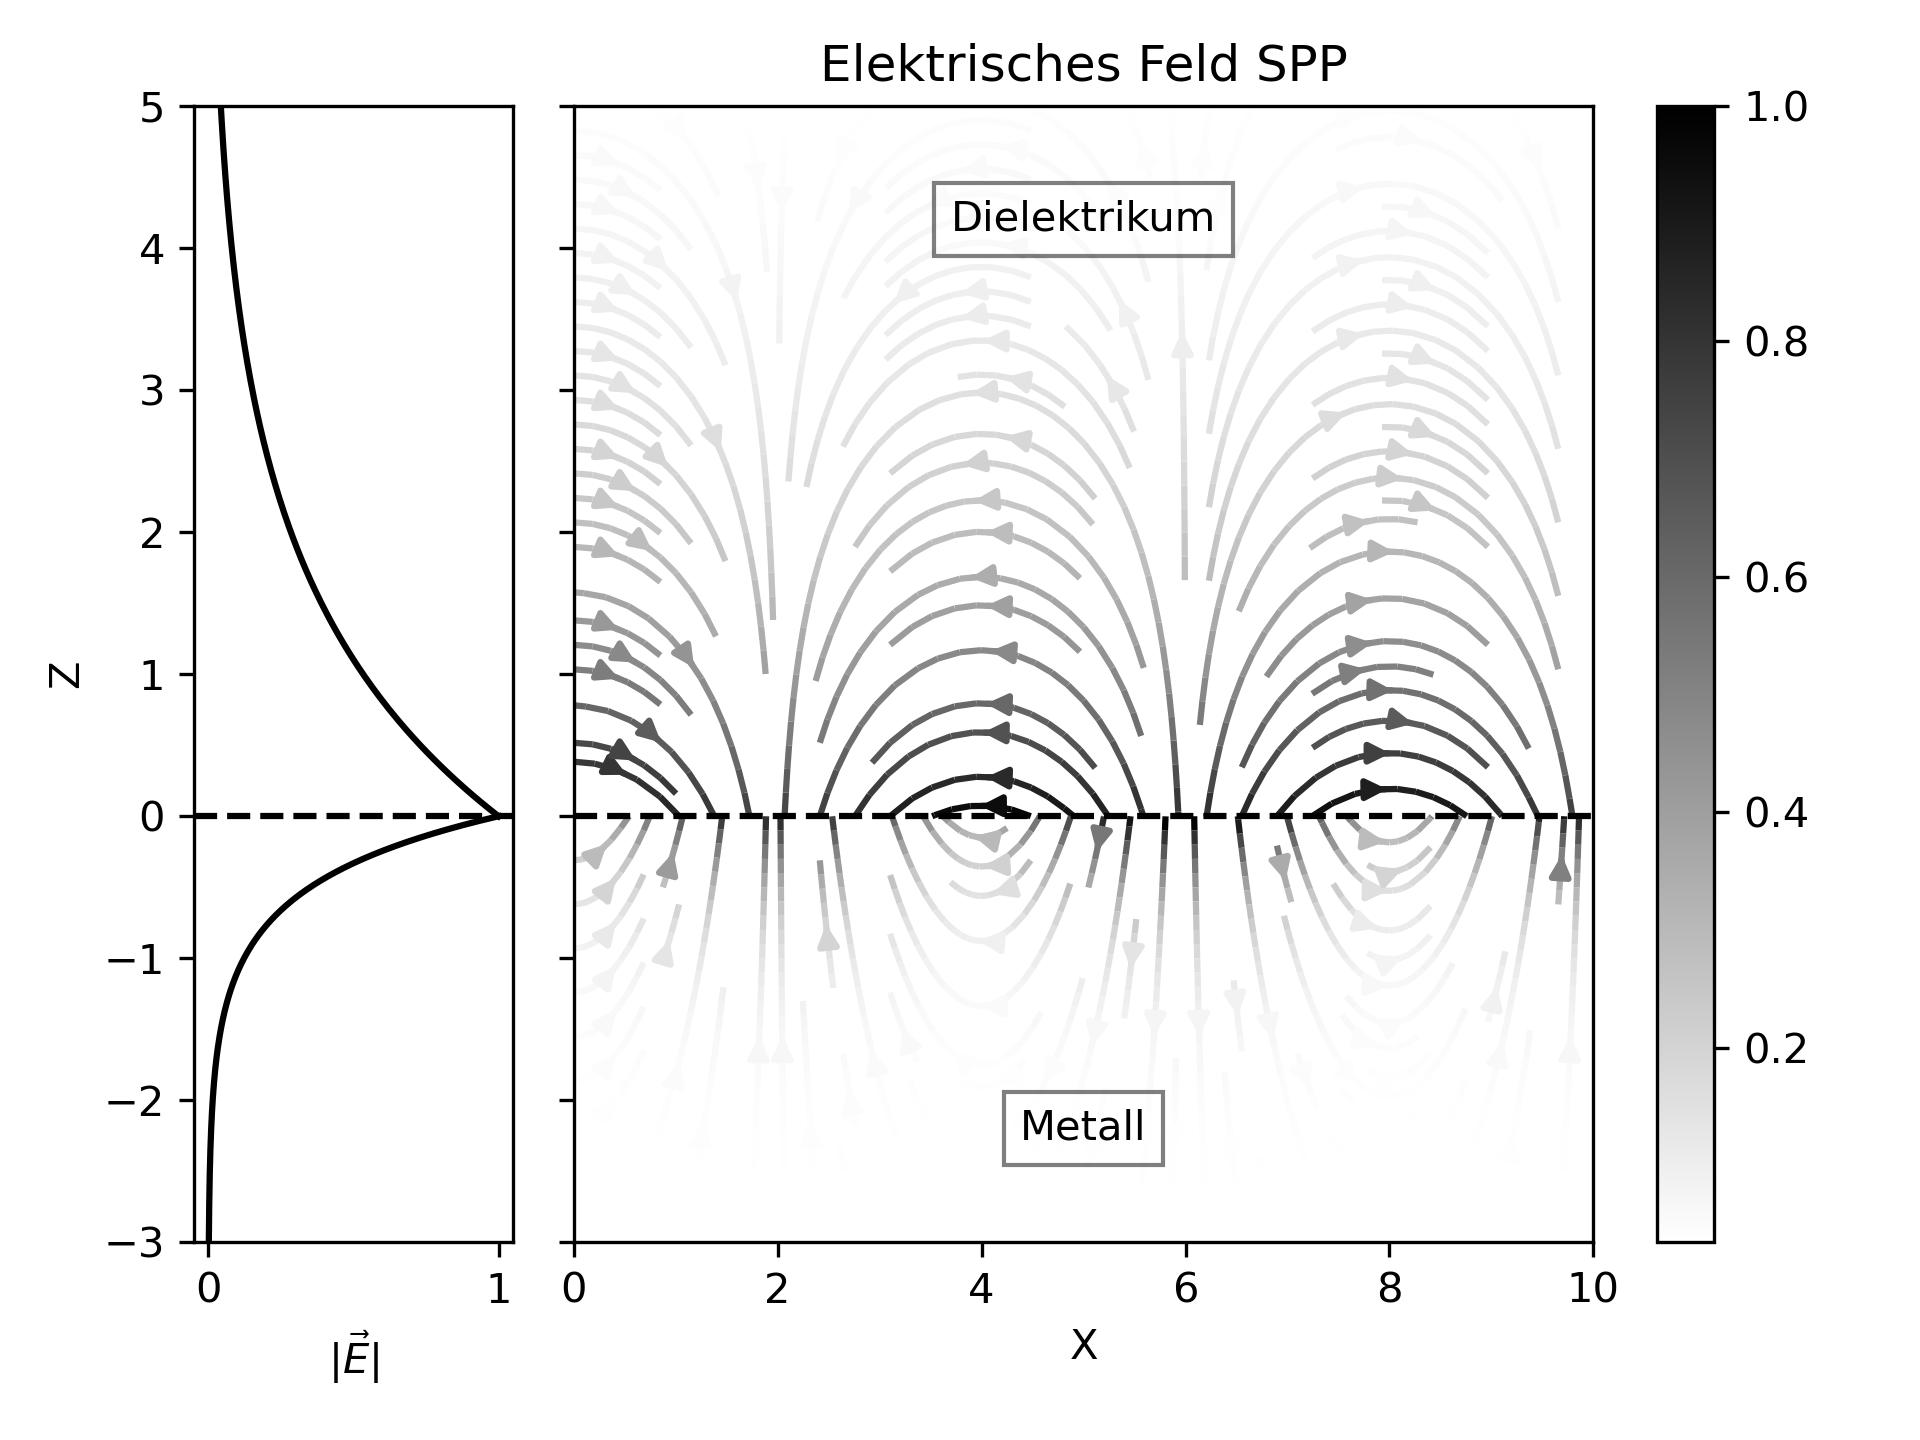
\includegraphics[width=0.7\textwidth]{figures/E_Feld_SPP.png}
		\caption{Quantitativer Verlauf der EM-Felder eines SPPs entlang einer Metall-Dielektrikums-Grenzschicht. Das Elektrische Feld ist durch die Pfeile dargestellt. Die Schwarz-Weiß Skala der Pfeile entspricht dem Betrag der Elektrischen Feldstärke. Die $y$-Komponente des Magnetfeldes ist durch die Farb-Skala dargestellt.}
		\label{fig:electric_field_spp}
	\end{figure}

	\subsubsection{Dispersion}
	Die Herleitung der Dispersionsrelation orientiert sich an den Ausführungen in \cite[pp.~261--ff]{Fox.2020} und kann dort im Detail nachvollzogen werden. Die Ausführungen in dieser Arbeit beschränken sich auf eine kurze Beschreibung des Vorgehens.
	Damit die oben angesetzten elektromagnetischen Felder \eqref{eq:electric_field_spp}, \eqref{eq:magnetic_field_spp}  die Maxwellgleichungen \eqref{eq:maxwell} und die Randbedingungen an der Grenzschicht erfüllen, müssen die Bedingungen \eqref{eq:condition_spp_1},  \eqref{eq:condition_spp_2} gelten. (Hierbei handelt es sich um den Spezialfall nicht magnetischer Materialien.)
	\begin{align}
		\label{eq:maxwell}	
		&\vec{\nabla}\cdot\vec{D} = 0		&\vec{\nabla}\cdot\vec{B} = 0 \\
		&\vec{\nabla}\times\vec{E} = -\dfrac{\partial\vec{B}}{\partial t} 
		&\vec{\nabla}\times\vec{H} = 	\dfrac{\partial\vec{D}}{\partial t}\nonumber
	\end{align}
	\begin{subequations}
		\begin{equation}
			\label{eq:condition_spp_1}
			\dfrac{k_{z, M}}{\epsilon_M} + \dfrac{k_{z, D}}{\epsilon_D} = 0
		\end{equation}		
		\begin{equation}
			\label{eq:condition_spp_2}
			k_{\mathrm{spp}}^2 +k_{z, n}^2 = \epsilon_n\left(\dfrac{\omega}{c}\right)^2; \text{ für  } n=M,D
		\end{equation}
		\end{subequations}
		$\epsilon_D$, $\epsilon_M = \epsilon_M(\omega) $ sind hierbei die Permittivitäten der Materialien in Abhängigkeit der Kreisfrequenz.
		Durch das Lösen der Bedingungen \eqref{eq:condition_spp_1},  \eqref{eq:condition_spp_2} ergibt sich die Dispersionsrelation des SPP an einer Grenzschicht zwischen einem Metall und einem Dielektrikum zu: 
		\begin{equation}
			\label{eq:dispersion_spp}
			\boxed{
				k_{\mathrm{spp}}\left(\omega\right) = \dfrac{\omega}{c} \sqrt{\dfrac{\epsilon_D\epsilon_M(\omega)}{\epsilon_D + 	\epsilon_M(\omega)}}  = k_0(\omega) n_{\mathrm{eff}}(\omega)}
		\end{equation}
		Hierbei ist $k_0 = \omega / c$ die Dispersion von elektromagnetischer Strahlung in Vakuum. Und $n_{\mathrm{eff}}(\omega)$ wird als effektiver Brechungsindex der Anregung bezeichnet. Die Dispersion kann über den Zusammenhang $E = \hbar \omega$ auch in Abhängigkeit der Energie dargestellt werden.
		
		 Aus Gleichung \eqref{eq:condition_spp_2} folgt $k_{z, n} = \sqrt{\epsilon_n k_0^2 - k_{\mathrm{spp}}^2}$. Diese Beziehung legt den Zusammenhang zwischen $k_{\mathrm{spp}}$ und $k_{z, n}$ fest. Außerdem lässt sich hieraus erkennen, dass für typische Materialien $ \operatorname{\mathbb{I}m}\{k_{z, n}\} \gg \Re\{k_{z, n}\}$. Durch die Dominanz des Imaginärteils über den Realteil der Wellenvektorkomponente senkrecht zur Ausbreitungsrichtung, fallen die Amplituden der Felder senkrecht zu Ausbreitungsrichtung exponentiell ab. Die Anregung ist daher stark an die Grenzfläche gebunden. 
	
	Im folgenden werden die Messdaten der Dielektrischen-Funktion von Gold aus der Publikation \cite{Olmon.2012} verwendet, um den Verlauf der Dispersion einer Vakuum-Gold und einer Glas-Gold Mode zu analysieren.  Die Publikation stellt Messdaten für unterschiedliche Gold-Oberflächenrauhigkeiten zur Verfügung. In dieser Arbeit wurden die Messdaten für aufgedampftes Gold verwendet. Für die Berechnung der Dispersion der Gold-Glas-Mode wurde $\epsilon_D = n_D^2 = 1.52^2$ und  verwendet. In der Dispersionskurve Abb. \ref{fig:dispersion_spp} ist zu erkennen, dass die Dispersionskurven bei einer Anregungs-Energie von $E = hc/\lambda_{\mathrm{HeNe}}= 1.95\mathrm{eV}$ jeweils rechts von der Lichtlinie des jeweiligen Materials liegen. Die starken Auswölbungen der Dispersionskurven bei $E > 2.4 \mathrm{eV}$ lassen sich durch Interbandabsorptionen erklären.
	\begin{figure}[h]
		\label{fig:dispersion_spp}
		\centering
		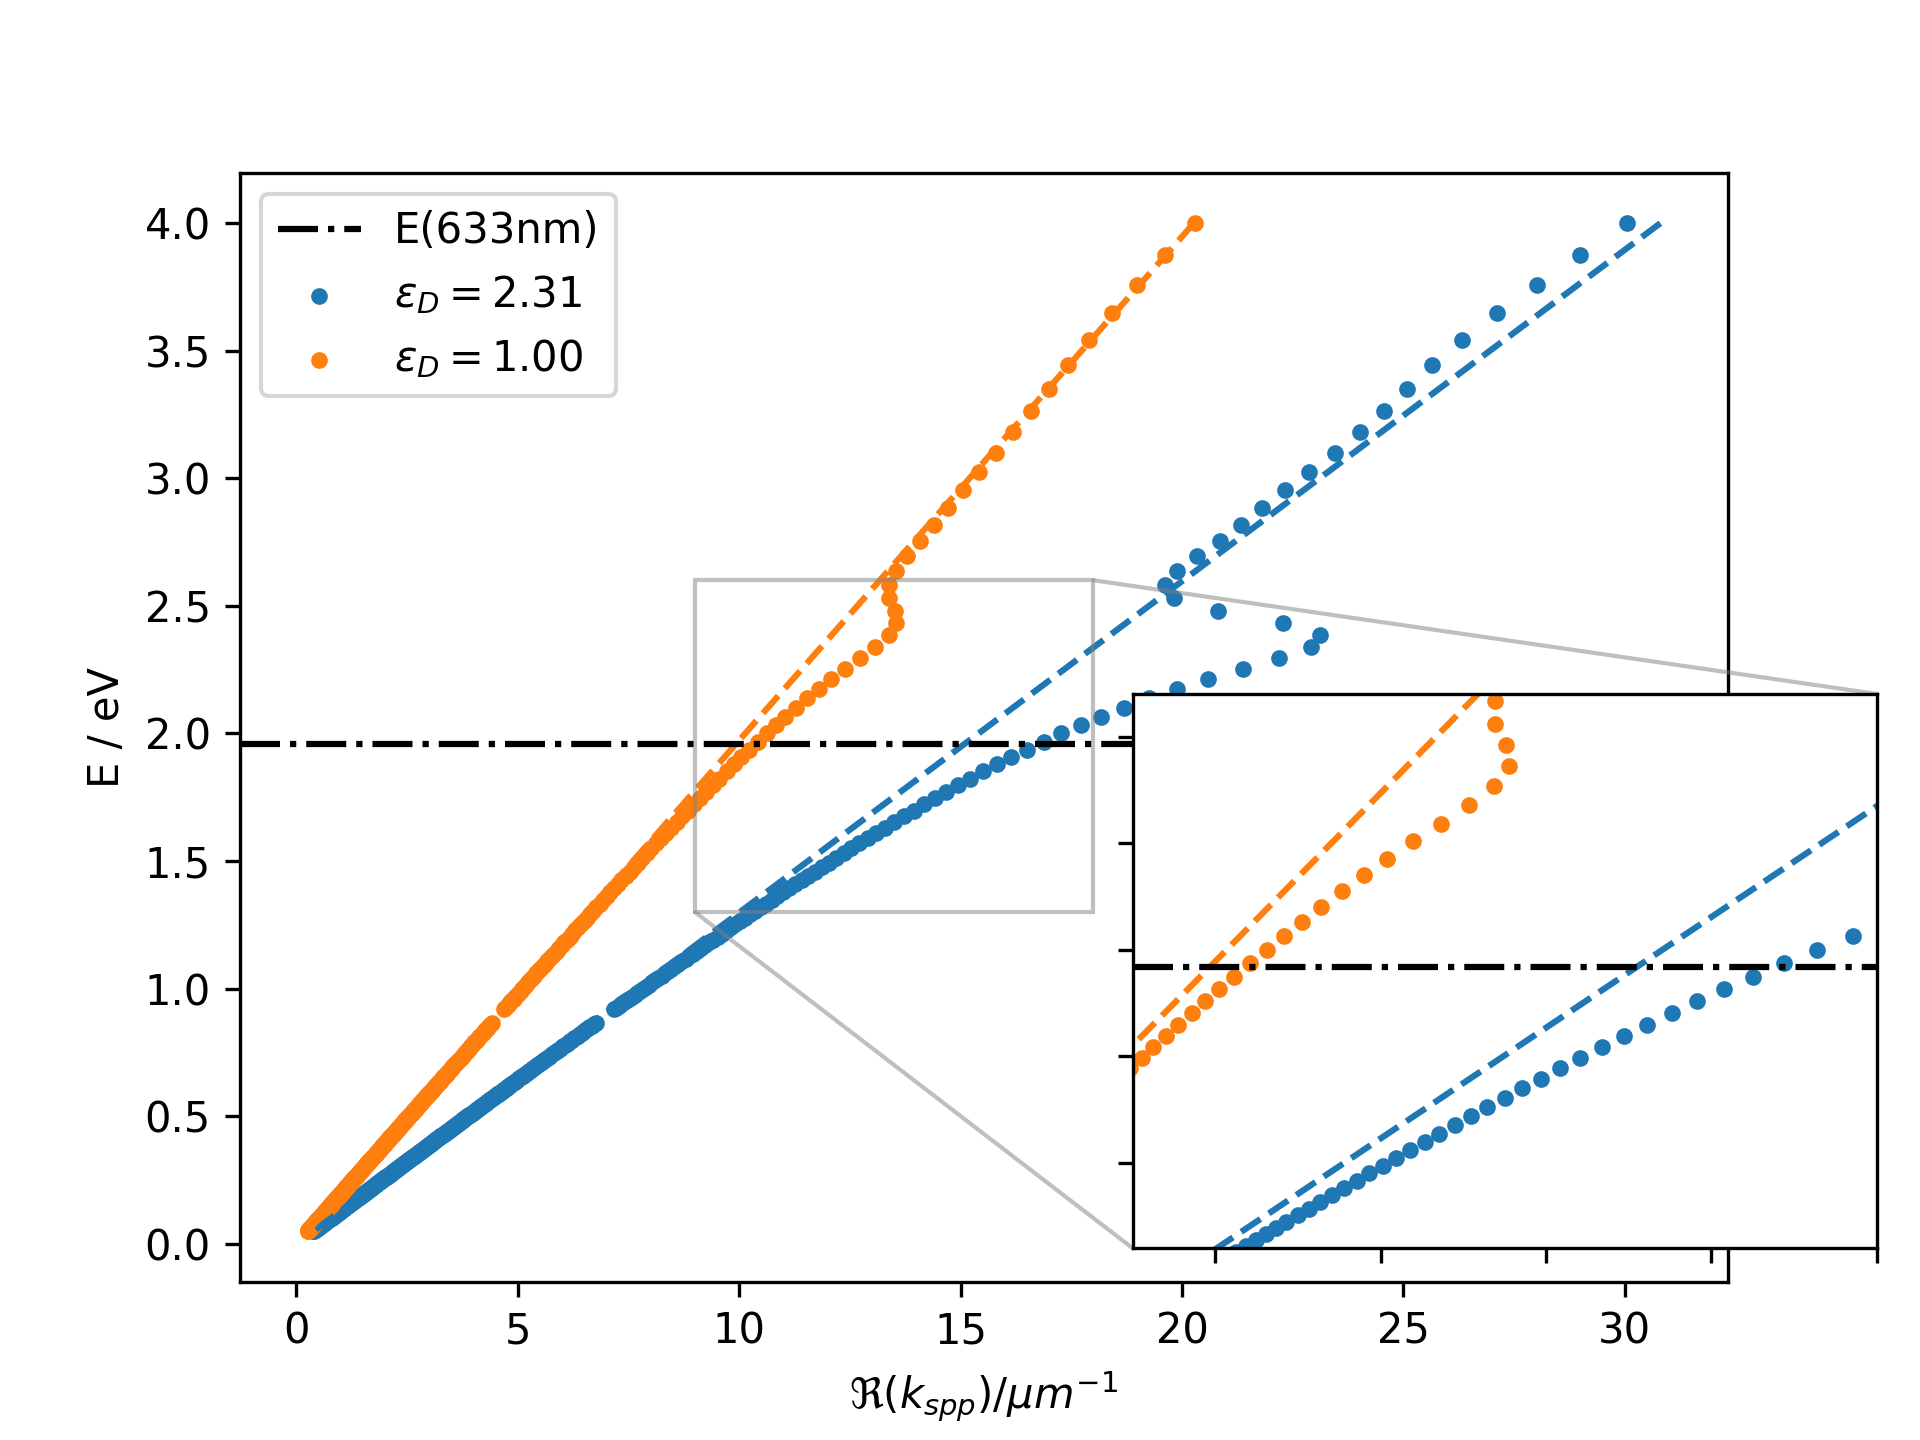
\includegraphics[width=0.7\textwidth]{figures/dispersion.png}
		\caption{Dispersionskurve der Gold-Vakuum und der Gold-Glas Mode. Die Lichtlinien im jeweiligen Medium sind zur Orientierung gestrichelt gekennzeichnet}		
	\end{figure}
	Die Differenz zwischen Dispersionskurve und Lichtlinie sorgt dafür, dass SPPs nicht ohne weiteres von Elektromagnetischer-Strahlung im jeweiligen Medium angeregt werden können.	
		\subsubsection{Anregung}
			Um trotz der k-Differenz in der Dispersionsrelation SPPs mit elektromagnetischer Strahlung anregen zu können, ist es notwendig, den k-Wert der Anregungsstrahlung zu erhöhen. Hierfür gibt es unterschiedliche Mechanismen:
			\paragraph{Kretschman-Konfiguration}
			In der Kretschmann Konfiguration wird ausgenutzt, dass man den auf eine Ebene projizierten Anteil eines Wellenvektors durch Variieren des Einfallswinkel verkleinern kann. Da der Wellenvektor allerdings vergrößert werden muss, um ein SPP mit EM-Strahlung aus dem Dielektrikum anzuregen, ist es notwendig ein System mit mehr als zwei Schichten zu verwenden. Ein dünner Metallfilm wird zwischen zwei Dielektrika mit $\epsilon_{D_1} > \epsilon_{D_2}$ eingeschlossen. So ist es möglich, den Wellenvektor der Anregenden Strahlung zunächst durch Wechsel in das Dielektrikum 1 zu vergrößern, und dann durch den Einfallswinkel zu Grenzschichtebene exakt an das SPP der Mode Metall-Dielektrikum 2 anzupassen. Dieses Verfahren wird bei der Kretschman-Konfiguration verwendet. Ein schematischer Aufbau der Kretschmann Konfiguration ist Abb. \ref{fig:kretschman} zu entnehmen.
				\begin{figure}[h] 
				\centering
				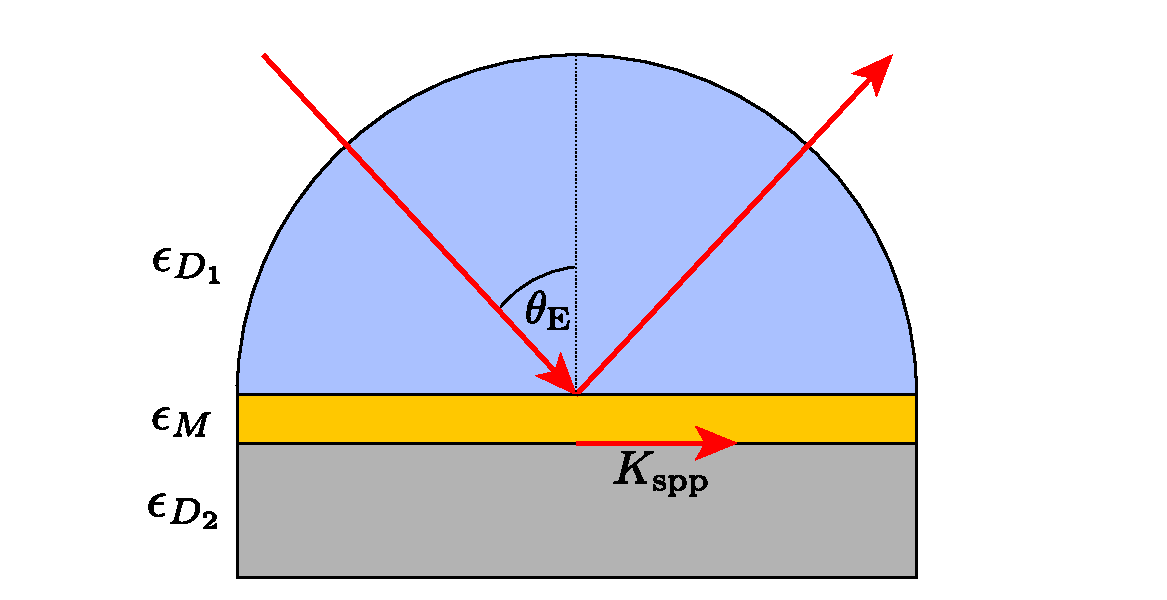
\includegraphics[width=0.5\textwidth]{figures/Kretschmann.pdf}
				\caption{Schematischer Aufbau der Kretschman-Konfiguration. Die Abbildung ist an \cite{Jaruschewski.2020} angelehnt}
				\label{fig:kretschman}
				\end{figure}
			Die Anregungsstrahlung tritt hier zunächst in das Medium mit $\epsilon_{D_1}$ ein. Hierdurch wird der Wellenvektor der Anregungsstrahlung auf $k_{D_1}=k_0\sqrt{\epsilon_{D_1}}$ vergrößert. Das Material des Prismas wird so gewählt, dass gilt:  $k_{D_1}> k_{\mathrm{SPP}}$ ($k_{\mathrm{SPP}}$ bezieht sich hierbei auf die Mode Metall-Dielektrikum 2 und ergibt sich aus \eqref{eq:dispersion_spp}) Der Einfallswinkel $\theta_E$ wird so gewählt, dass die Projektion von $k_{D_1}$ auf die Goldoberfläche exakt $k_{\mathrm{SPP}}$ entspricht. Es gilt also:
			\begin{align}
				\label{eq:phase_condition_kretschmann}
				\sin(\theta_E) &= \dfrac{\Re\{k_{\mathrm{spp}}\}}{k_{D_1}}\\
				\Rightarrow \Re\{k_{\mathrm{SPP}}\} &= \sin(\theta_E) k_0 \sqrt{\epsilon_{D_1}}
			\end{align}
			Damit diese Phasen-Anpassungs-Bedingung erfüllbar ist, ist es notwendig, dass gilt: $\sqrt{\epsilon_\mathrm{D_1}} > n_\mathrm{eff, SPP}$
			Bei der Reflektion einer elektromagnetischen Welle an einem Metall, dringen in das Metall evaneszente Felder ein. \cite{Novotny.2012b}. Ist die Metallschicht dünn genug, haben diese evaneszenten Felder an unteren Grenzfläche des Metalls noch ausreichend Intensität, um dort ein SPP anzuregen. Dies ist möglich, da die k-Komponenten wie oben erläutert an einander angepasst worden sind. Die in Abb. \ref{fig:kretschman} gezeigte Geometrie nutzt für das Dielektrikum 1 einen Halbkreis, damit der Stahl unabhängig vom Winkel $\theta_\mathrm{E}$ senkrecht in das Dielektrikum 1 eintritt. Als Dielektrikum 2 wird häufig Vakuum oder Luft verwendet.			
		
			\paragraph{Anregung an Strukturen}
			Eine weitere Möglichkeit, die Wellenvektordifferenz zu überwinden stellen, scharfe Strukturen in oder an der Metalloberfläche da. Scharfe Strukturen im Ortsraum besitzen gemäß den Gesetzen der Fouriertransformation ein breites Raumfrequenzspektrum. Diese breite Raumfrequenzspektrum kann durch Streuprozesse an die Elektromagnetische Strahlung übertragen werden, die so die nötige Wellenvektordifferenz überwinden kann, um ein SPP anzuregen. Der Streuprozess an einem kleinem Partikel auf der Goldoberfläche kann in erster Näherung als abstrahlender Dipol aufgefasst werden. Dieser Prozess wird detaillierter in \Cref{sec:spatial_freq_dip} anhand des Raumfrequenzspektrums eines Dipols dargestellt.
		\subsubsection{Leckstrahlung}
		\label{sec:leakage_radiation}
			Leckstrahlung ist der inverse Effekt zur Anregung in der Kretschmann-Konfiguration. In einem Dreischichtsystem Dielektrikum2-Metall-Dielektrikum1 kann ein an der Grenzfläche Dielektrikum2-Metall propagierendes SPP durch evaneszente Felder EM-Felder an der Grenzfläche Metall-Dielektrikum1 erzeugen. Diese Felder können EM-Strahlung im Dielektrikum1 unter dem Winkel $\theta_\mathrm{L}$ erzeugen. Dieser Winkel muss analog zu \eqref{eq:phase_condition} folgende Phasenanpassungsbedingung erfüllen:
			\begin{equation}
				\label{eq:phase_condition}
				\boxed{\Re\{k_{\mathrm{spp}}\}=\sin(\theta_\mathrm{L}) k_0 \sqrt{\epsilon_{D_1}}}
			\end{equation}
			Damit die Wellenvektorkomponenten des SPPs und der Leckstrahlung übereinstimmen.
			 Dies ist nur möglich, wenn {$\sqrt{\epsilon_{D_1}} > \Re\{n_\mathrm{eff, SPP}\}$} ist. Diese in das Dielektrikum 1 abgestrahlte Strahlung bezeichnet man als Leckstrahlung. Für das Auftreten von Leckstrahlung muss der Metallfilm hinreichend dünn sein, damit die evaneszenten Felder des  SPP an der zweiten Grenzschicht noch ausreichend Intensität aufweisen, um in das Dielektrikum auszukoppeln. Durch die Phasenanpassungsbedingung \eqref{eq:phase_condition} kann einem Bestimmten Abstrahlwinkel $\theta_L$ ein konkreter $\Re\{k_{\mathrm{SPP}}\}$ zugeordnet werden und umgekehrt. Dieser Umstand wird bei der Leckstrahlmikroskopie ausgenutzt, um den Wellenvektor des SPP zu bestimmen. Das Auftreten von Leckstrahlung ist also ein nützlicher Effekt, um SPPs mit optischen Instrumenten zu beobachten.
				\begin{figure}[h] 
				\centering
				\includegraphics[width=0.5\textwidth]{figures/leckstrahlung.pdf}
				\caption{Abstrahlung von Leckstrahlung in einem Drei-Schichtsystem}
				\label{fig:leakage_radiation}
			\end{figure}
		\subsubsection{Berechnung von charakteristischen Größen für das System Luft-Gold-Glas}
		Alle in dieser Arbeit durchgeführten Messungen wurden am System Luft-Gold-Glas durchgeführt. Daher werden an dieser Stelle die oben Eingeführten Größen für dieses System angegeben. Die Dielektrizitätskonstante des Glases ist $\epsilon_{\mathrm{G}} = 2.327$ \cite{Zeiss.} und die von Luft ist $\epsilon_{\mathrm{L}} = 1.00059$ \cite{Hippel.1995}. Die dielektrische Funktion von Gold wurde bei einer Anregungsenergie von $E_{\mathrm{HeNe}} = h\lambda/c = 1.96\mathrm{eV} $ durch Interpolation der Messdaten aus der Publikation \cite{Olmon.2012} berechnet: $\epsilon_{\mathrm{Au}}(1.96\mathrm{eV}) = -12.04 +1.163i$ Aus diesen Daten lassen sich nun folgende Größen berechnen:
		\begin{subequations}
			\begin{align}
				n_{\mathrm{eff}} &= \sqrt{\dfrac{\epsilon_{\mathrm{L}}\epsilon_{\mathrm{Au}(\omega)}}{\epsilon_{\mathrm{L}} + 	\epsilon_{\mathrm{Au}}(\omega)}} = 	1.044 + 0.005i \label{eq:theo_n_eff}\\			
				\theta_\mathrm{L} &=  \arcsin\left(\dfrac{\Re(n_{\mathrm{eff}})}{ n_\mathrm{G}}\right) = 43.2^\circ 
				\label{eq:theo_theta_l}\\
				k_{\mathrm{SPP}} &= k_0 n_{\mathrm{eff}} = (10.365 + 0.0449i)\mathrm{\mu m}^{-1}\label{eq:theo_k_spp}
			\end{align}
		\end{subequations}
	\subsection{Plasmonischer-Spin-Hall-Effekt (PSHE)}
	Als Plasmonische-Spin-Hall-Effekt wird der bezeichnet, dass an einer räumlich symmetrischen Struktur angeregte SPPs, abhängig von der Polarisation der anregenden Strahlung, bevorzugt in unterschiedliche Richtungen propagieren. Speziell propagiert das SPP bei links-zirkular polarisierter Strahlung in eine um 180° verschiedene Richtung zu dem SPP, dass mit rechts zirkular polarisiertem Licht angeregt worden ist. Der PSHE kann durch zwei verschiedene Vorgehensweisen erklärt werden. Ein Weg ist, die Struktur, an der SPPs angeregt werden durch einen zirkular polarisierten Dipol zu nähern. Das Fernfeld eines zirkular polarisierten Dipols ist isotrop. Daher ist es zunächst verwunderlich, dass ein zirkular polarisierter Dipol zu einer gerichteten Anregung führen kann. Bei genauerem Betrachten des Dipol-Feldes fällt allerdings auf, dass das Nahfeld nicht isotrop ist. Wenn nun ein SPPs unterstützendes Schichtsystem in diese Nahfeld des Dipols gebracht wird, kann diese Anisotropie zu einer gerichteten Anregung führen.
	Eine weitere Vorgehensweise den Effekt zu erklären ist es, über die Erhaltung des Spins zu argumentieren. Das Photon hat vor der Wechselwirkung mit der Struktur einen Longitudinalen Spin, der je nach Drehsinn der zirkularen Polarisation in oder entgegen der Ausbreitungsrichtung des Photons zeigt. Das SPP hat einen Spin, der transversal auf seiner Ausbreitungsrichtung steht. Damit der Spin nach der Wechselwirkung nicht seine Richtung ändert, ist also eine gerichtete Anregung notwendig.
	\subsubsection{Raumfrequenzspektrum von Elektromagnetischen-Feldern}
		Um den Plasmonischen-Spin-Hall-Effekt zu verstehen, wird die Raumfrequenzdarstellung von Elektromagnetischen Feldern benötigt. Die folgenden Ausführungen orientieren sich an \cite{Novotny.2012b}, wobei in dieser Arbeit nur der etwas einfacherer 2D-Fall diskutiert wird.\\		
		Das Elektrische Feld am Ort $\vec{r} = (x, y) $ sei durch $\vec{E}({\vec{r}})$ gegeben.
		Die Zeitabhängigkeit von $\vec{E}$ sei durch $\vec{E}({\vec{r}, t})=\Re\{\vec{E}({\vec{r}})\exp(-i\omega t)\}$ gegeben. Dann lässt sich $\vec{E}({\vec{r}})$ durch eine Fouriertransformation in $x$-Richtung wie folgt darstellen:
		\begin{equation}
			\label{eq:Exz_fourier}
			\vec{E}(x,z) = \int_{-\infty}^{\infty}\mathrm{d}{k_x}\hat{\vec{E}}(k_x,z)\exp(ik_xx)				
		\end{equation}
		\begin{equation}
			\label{eq:EKxz_fourier}
			\hat{\vec{E}}(k_x,z) = \dfrac{1}{2\pi}\int_{-\infty}^{\infty}\mathrm{d}x\vec{E}(x,z)\exp(-ik_xx)
		\end{equation}
		Wenn wir davon ausgehen, dass das Medium entlang der $x$-Achse homogen, isotrop, linear und quellfrei ist, muss das Elektrische Feld, die sich unter diesen Bedingungen aus den Maxwellgleichungen \eqref{eq:maxwell} ergebende Helmholtz-Gleichung $(\vec{\nabla}^2+k^2)\vec{E}({\vec{r}}) = 0$, erfüllen. Einsetzen von \eqref{eq:Exz_fourier} in die Helmholtz-Gleichung ergibt mit der Definition $k_z := \sqrt{k^2-k_x^2}$ folgenden Zusammenhang:
		\begin{equation}
			\label{eq:spatial_spektrum}
		\hat{\vec{E}}(k_x,z) =\hat{\vec{E}}(k_x,z= 0) \exp(\pm ik_ z)
		\end{equation}
	Das Vorzeichen legt hier die Propagationsrichtung fest.
	Einsetzen in \eqref{eq:Exz_fourier} ergibt:
		\begin{equation}
			\label{eq:Espatial_spektrum}
			\vec{E}(x,z) = \int_{-\infty}^{\infty}\mathrm{d}{k_x}\hat{\vec{E}}(k_x,z= 0)\exp(i(k_xx\pm k_ z))
		\end{equation}
	Wenn also das Raumfrequenzspektrum für einen z-Wert bekannt ist, lassen sich die Spektren für alle anderen z-Werte gemäß \eqref{eq:spatial_spektrum} berechnen. Für einen festen Wert von $k_x$ gibt es, je nach dem ob $k_x$ größer oder kleiner als $k$ ist zwei unterschiedliche Lösungen. Wenn $k_x^2 < k^2$ ist, ist $k_z := \sqrt{k^2-k_x^2}$ eine reelle Zahl. Daher handelt es sich nach \eqref{eq:spatial_spektrum} um eine ebene Welle, die entlang der z-Achse propagiert.
	Wenn hingegen $k_x^2 > k^2$ ist, ist $k_z := \sqrt{k^2-k_x^2}$ eine imaginäre Zahl. Dann handelt es sich bei \eqref{eq:spatial_spektrum} um eine evaneszente Welle, die entlang der z-Achse exponentiell abklingt. In dem Raumfrequenzspektrum kann man also zwischen Bereichen mit Ebenen-Wellen und  Bereichen mit Evaneszenten-Wellen unterscheiden. Dieses Konzept lässt sich ohne weiteres auch auf 3 Raumdimensionen und das Magnetische Feld erweitern.
	\subsubsection{Raumfrequenzspektrum der Elektromagnetische Strahlung eines oszillierenden Dipols}
		\label{sec:spatial_freq_dip}
		Wenn man das oben beschriebene Verfahren auf einen Elliptisch-Polarisierten Dipol anwendet, lässt sich das Raumfrequenzspektrum bestimmen. Hier werde ich mich wieder auf den 2-Dimensionalen Fall beschränken. Das zeitabhängige Dipolmoment sei: 
		$$\vec{P}(t)= \Re\left[\underbrace{\begin{pmatrix} p_x \\ p_z \end{pmatrix}}_{\vec{P}} \exp(-i\omega t)\right]$$
		$p_x$ und $p_y$ sind im allgemeinen komplexe Zahlen. So kann $\vec{P}$ auch Elliptische Polarisationen darstellen. Das Die y-Komponente des Magnetfeldes dieses Dipols lässt sich nun, wie in \cite{Novotny.2012b} und \cite{RodriguezFortuno.2013} gezeigt wird, analog zu den obigen Ausführungen in Raumfrequenzanteile zerlegen.
		\begin{equation}
			H_y(x, z) = \int_{-\infty}^{\infty}\mathrm{d}k_x\hat{H_y}(k_x, z)\exp(ik _xx) 
		\end{equation}
		mit
		\begin{equation}
			\boxed{\hat{H_y}(k_x, z) = \dfrac{i\omega}{8\pi^2}\left\{p_z\dfrac{k_x}{k_z} \mp p_x\right\}\exp(ik_z|z-z_{\mathrm{Dipol}}|)}
		\end{equation}
	$z_{\mathrm{Dipol}}$ ist hierbei die Position des Dipols auf der $z-Achse$. $k_z$ lässt sich wieder über die Differenz von $k_x$ zur Gesamtwellenzahl $k$ berechnen. $k_z := \sqrt{k^2-k_x^2}$ Wenn $k_x$ schon den gesamten Anteil der Gesamtwellenzahl "aufgebraucht" wird $k_z$ imaginär und die resultierende Welle deswegen evaneszent. Wenn $k_x$ einen Anteil der Gesamtwellenzahl "übrig" lässt, bleibt $k_z$ reell und die Welle kann propagieren. Ähnlich wie bei der Leckstrahlung, ergibt sich ein durch die Phasenanpassungsbedingung ein Winkel zur $z$-Achse, unter dem die Welle mit bestimmten $k_x$ propagiert: $\theta = \arcsin(k_x/k)$. Da $k = \omega / c$  hängt das Raumfrequenzspektrum nur von dem äußeren Parameter $\omega$ bzw. $k$ ab. 
	\paragraph{Analyse des Dipol-Raumfrequenzspektrums}
		Die Analyse des Raumfrequenzspektrums erfolgt in dieser Arbeit rein quantitativ unter Verwendung von willkürlichen Einheiten. Der Real und Imaginär Teil des Raumfrequenzspektrums in einer halben Wellenlänge unterhalb des Dipols lässt sich nun numerisch darstellen. $k_x$ wurde hierbei in Einheiten von $k$ dargestellt. Dann ist für das Intervall $-1 < k_x / k <1$ $k_z$ real. Dieses $k_x$ Intervall entspricht also propagierenden Wellen. Die Raumfrequenzspektrums-Amplitude wurde in dem Bereich der Darstellung auf 1 normiert.
		\subparagraph{Linear polarisierte Dipol in $x$-Richtung}
			Der Dipol sei:
			 $$\vec{P} = \begin{pmatrix} 1 \\ 0\end{pmatrix}$$
			Das Raumfrequenzspektrum des in x-Richtung orientierten Dipols weist eine gerade Parität auf, ist also achsensymmetrisch.	
		\subparagraph{Linear polarisierte Dipol in $z$-Richtung}
			Der Dipol sei:
			$$\vec{P} = \begin{pmatrix} 0 \\ -i\end{pmatrix}$$
			Das Raumfrequenzspektrum dieses Dipols zeigt ungerade Parität, ist also punktsymmetrisch um den Ursprung.
		\begin{figure}
			\centering
			\label{fig:spatial_spectrum_zx}
			\begin{subfigure}[h]{0.49\textwidth}
				\centering
				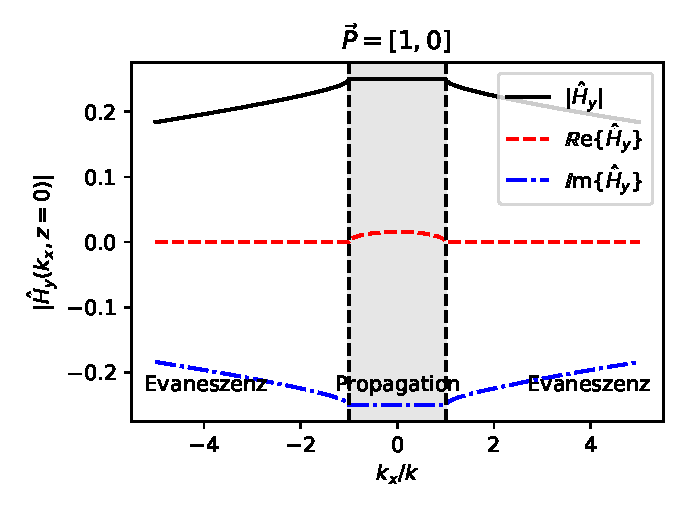
\includegraphics[width=\textwidth]{figures/spatial_spectrum_x.pdf}
				\caption{Orientierung in x-Richtung}
				\label{fig:spatial_spectrum_x}
			\end{subfigure}		
			\begin{subfigure}[h]{0.5\textwidth}
				\centering
				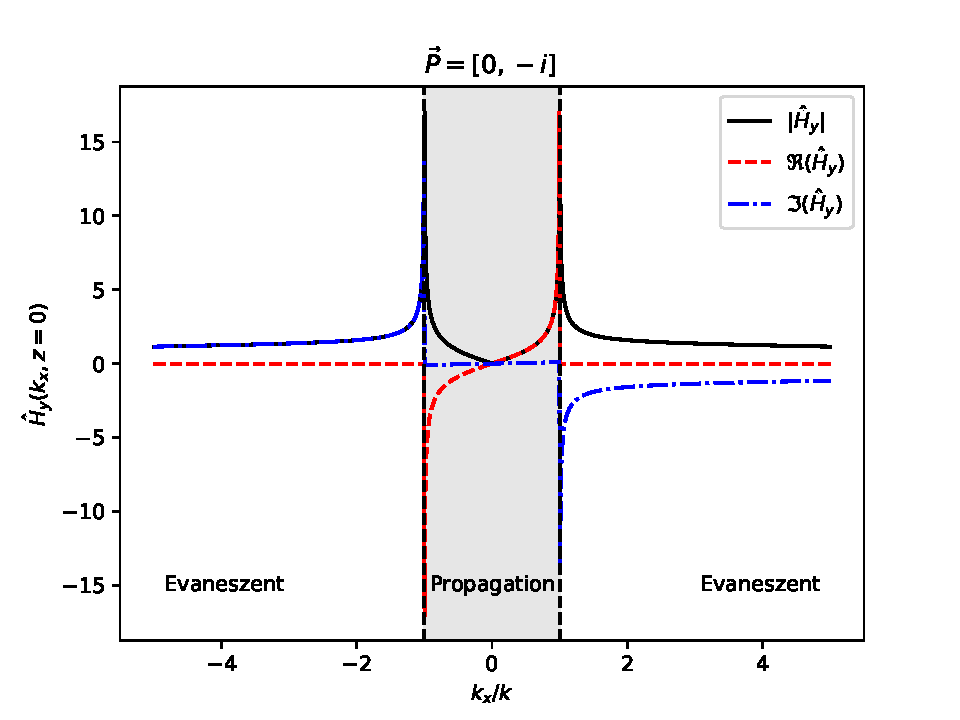
\includegraphics[width=\textwidth]{figures/spatial_spectrum_z.pdf}
				\caption{Orientierung in z-Richtung}
				\label{fig:spatial_spectrum_z}
			\end{subfigure}		
			\caption{Das Raumfrequenzspektrum von  einem linear polarisierten Dipol zeigt je nach Orientierung des Dipols unterschiedliche Parität. In rot ist jeweils der Realteil, in blau der Imaginärteil und in Schwarz der Betrag des jeweiligen Spektrums dargestellt.}		
		\end{figure}
		\subparagraph{Zirkular polarisierte Dipol}
			Der Dipol sei:
			$$\vec{P} = \begin{pmatrix} 1 \\ -i\end{pmatrix}$$
			Das Raumfrequenzspektrum aus der phasenverschobenen Überlagerung der beiden Dipole ist asymmetrisch. Im negativen x-Bereich überlagern sich die Spektren destruktiv, im positiven Bereich konstruktiv. Wenn nun sehr nah an dem Zirkular polarisierten Dipol ein Schichtsystem, dass die Anregung von SPPs unterstützt positioniert wird, kann durch den Teil des Spektrums der $k_{\mathrm{SPP}}$ entspricht ein SPP angeregt werden. Das Vorzeichen von $k_{\mathrm{SPP}}$ entspricht hierbei der Anregungsrichtung des SPPs. Da $\hat{H}_y(k_{\mathrm{SPP}}) \neq \hat{H}_y( -k_{\mathrm{SPP}}) $ findet die Anregung bevorzugt in eine Richtung statt. Diese Richtung ist abhängig von dem Drehsinn des zirkular polarisierten Dipols.			
			Das Nahfeld eine zirkular polarisiertem Dipols ist also anisotrop, obwohl das Fernfeld welches man durch substituieren von $k_x = k_o \sin(\theta)$ erhält, isotrop ist. Damit diese Orientierung des Dipols in der Struktur ermöglicht wird, ist ein streifender Einfall notwendig. Erst der Streifende Einfall bring den nötigen Symmetriebrechung für eine gerichtete Anregung.
		\begin{figure}[h]
			\centering
			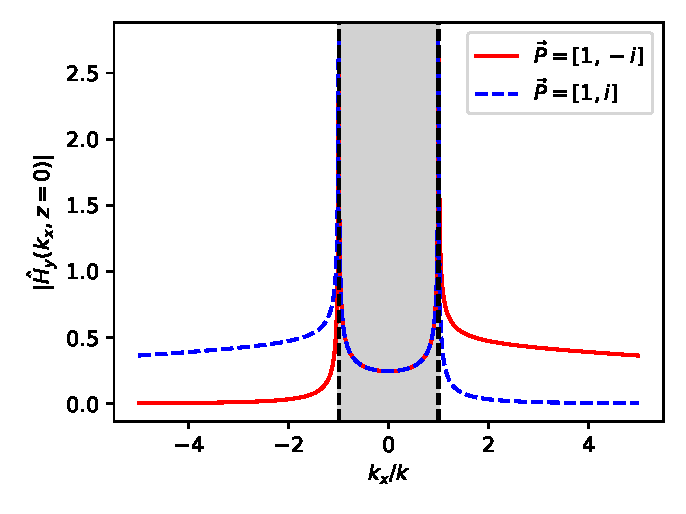
\includegraphics[width=0.7\textwidth]{figures/spatial_spectrum_circ.pdf}
			\caption{Raumfrequenzspektrum eines zirkular polarisierten Dipols bei unterschiedlichem Drehsinn der Polarisation}
			\label{fig:spatial_spectrum_circ}
		\end{figure}	
		
	
		
	\subsubsection{Analyse des Drehmomentes von elektromagnetischer Strahlung}
	Elektromagnetische Strahlung kann Impuls und Drehmoment transportieren. Das Drehmoment übersetzt sich nach dem Quantenmechanischen-Korrespondenzprinzip in einen Spin. Im folgenden wird daher im klassischen Bild das Drehmoment von unterschiedlichen Elektromagnetischen-Strahlungsarten analysiert.
	\paragraph{Propagierende-Ebene-Wellen}
		Propagierende EM-Wellen transportieren abhängig von ihrer Polarisation ein Drehmoment. Linear polarisierte EM-Wellen besitzen kein Drehmoment. Ihr Elektrischen und Magnetischer Feldvektor oszilliert jeweils nur in einer Ebene.
		 
		Bei elliptisch polarisierten Elektromagnetischen Wellen hingegen rotiert der Elektrische-Feld-Vektor an einem festen Ort mit dem fortschreiten der Zeit. Das gleiche gilt auch für den magnetischen Feldvektor. Diese Felder können daher eine Referenzteilchen in Rotation versetzten und transportieren dementsprechend auch einen Drehimpuls. Da die Rotation nur in Ebenen senkrecht zur Ausbreitungsrichtung stattfindet, ist der Drehimpuls parallel bzw. antiparallel zur Ausbreitungsrichtung der EM-Welle. Daher haben elliptisch polarisierte propagierende Elektromagnetische Felder einen Longitudinalen Spin.
		
		\begin{figure}[h]
			\centering
			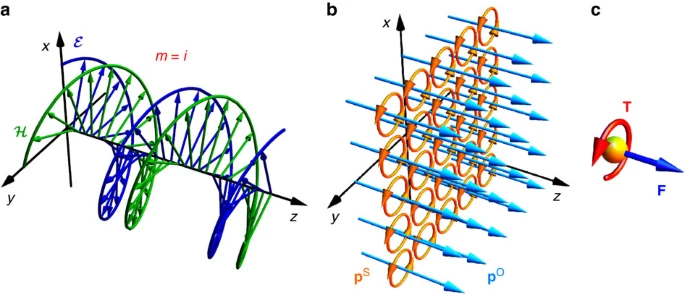
\includegraphics[width=0.7\linewidth]{figures/spin/prop_spin}
			\caption{Der Elektrische Feldvektor einer propagierenden zirkular polarisierten Welle beschreibt bei festgehaltener Zeit eine Helix Bahn entlang der Ausbreitungsrichtung. An einem festgehaltenen Ort beschreibt der Elektrische Feldvektor also eine Kreisbahn senkrecht zur Ausbreitungsrichtung. Die Abbildung ist aus \cite{Bliokh.2014} übernommen.}
			\label{fig:prop_spin}
		\end{figure}
		
	\paragraph{Evaneszente-Wellen}	
	Evaneszente Elektromagnetische Felder weisen hingegen unabhängig von ihrer Polarisation einen Spin in Transversaler Richtung auf. Wenn man bei einer evaneszenten Elektromagnetischen Welle den zeitlichen Verlauf des elektrischen Feldvektors $\vec{E}(t)$ an einem festen Ort beobachtet, stellt man fest, dass $\vec{E}(t)$ in der $zx$-Ebene schwingt. Der Elektrische Feldvektor rotiert hier also in einer Ebene parallel zur Ausbreitungsrichtung. Das Drehmoment steht hier also senkrecht auf der Ausbreitungsrichtung. \cite{Bliokh.2014}
	
		
	\begin{figure}[h]
		\centering
		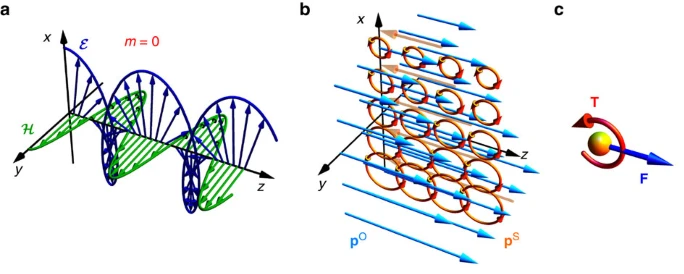
\includegraphics[width=0.7\linewidth]{figures/spin/ev_spin}
		\caption{Der Elektrische Feldvektor einer evaneszenten Welle beschreibt bei festgehaltener Zeit eine Zykloide in der $xz$-Ebene. An einem festgehaltenen Ort beschreibt der Elektrische Feldvektor also eine Kreisbahn.}
		\label{fig:ev_spin}
	\end{figure}
	\paragraph{Spin-Erhaltung beim Plasmonischen-Spin-Effekt}
		Durch den streifenden Einfall des zirkularpolarisierten Lasers ist hat der Gesamtspin des Photons vor der Wechselwirkung mit dem Nanopartikel ein $x$-Komponente. Je nach dem, ob das resultierende SPP in $+y$-Richtung oder in $-y$-Richtung propagiert, hat das SPP einen Gesamtspin in  $+x$ oder $-x$ Richtung. Die Propagationsrichtung wird sich nun so ergeben, dass der Gesamtspin bei der Interaktion mit dem Nanopartikel erhalten bleibt. Da eine Umkehr des Drehsinns der Polarisation der anregenden Strahlung auch zu einer Umkehr des Spins der anregenden Strahlung führt, führt ein umgekehrter Drehsinn zu unterschiedlichen Propagationsrichtungen des SPPs.
		\begin{figure}[h]
			\centering
			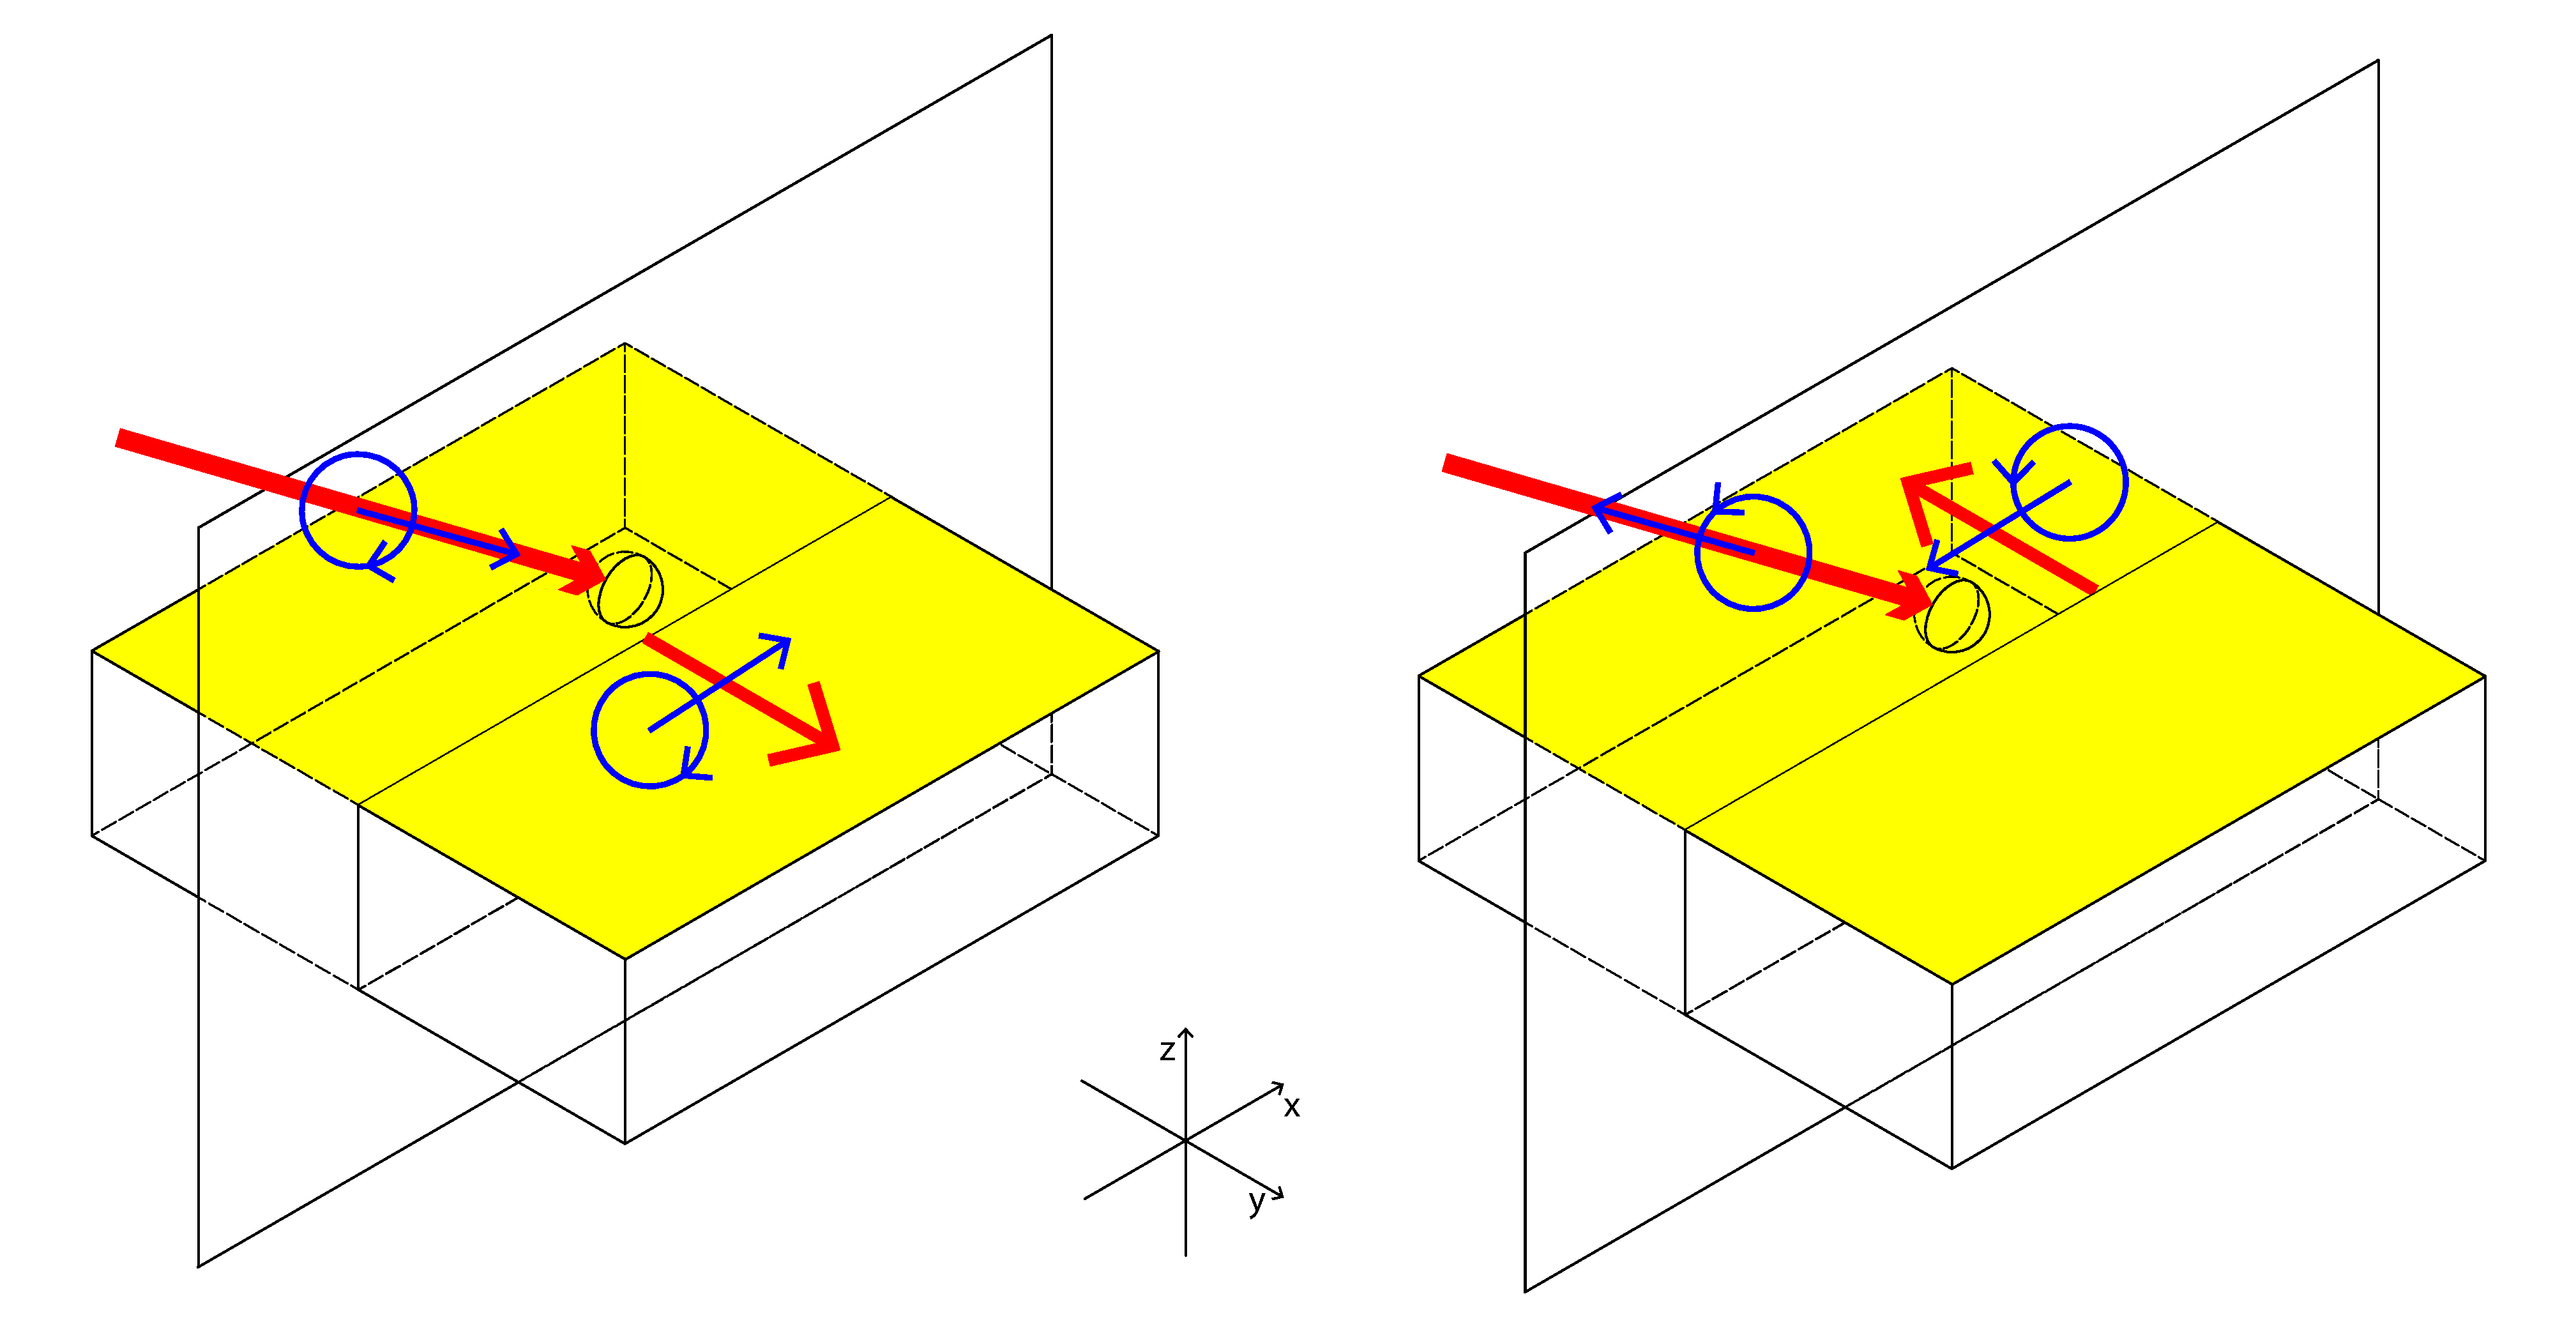
\includegraphics[width=1.0\linewidth]{figures/spin_hall_schema.pdf}
			\caption{Spin-Erhaltung beim Plasmonischen-Spin-Hall Effekt. In Blau ist jeweils der Spin des Plasmons und der anregenden Strahlung gekennzeichnet.}
			\label{fig:spin_hall_schema}
		\end{figure}


 	
\section{Messung und Methoden}
\subsection{Leckstrahlmikroskopie}
	In dieser Arbeit wurde ein Leckstahlmikroskop verwendet, um den plasmonischen Spin-Hall Effekt experimentell nachzuweisen. Ein LRM hat gegenüber anderen Methoden zur Untersuchung Plasmonischer Systeme den Vorteil, dass es rein optisch arbeitet und deswegen nicht auf aufwendige Vakuum-Technik angewiesen ist. Ein Leckstahlmikroskop nutzt aus, dass SPPs in einem Mehrschichtsystem wie in \Cref{sec:leakage_radiation} erläutert, Leckstrahlung unter einem spezifischen Winkel in ein Substrat abstrahlen können. Als Probe wurde in dieser Arbeit ein auf ein Glassubstrat aufgedampfter Goldfilm verwendet. Das Schichtsystem ist also Luft-Gold-Glas.
	
	Ein Defekt auf der Probe wird zunächst von der Luftseite mit einem Laser bestrahlt. An der Luft-Gold Grenzflächen werden hierdurch SPPs angeregt. Diese SPPs strahlen nun Leckstrahlung in das Glassubstrat ab.
	Außerdem wird ein Teil des Lasers direkt transmittiert. Auf der Glasseite der Probe wird mit einem Immersionsobjektiv die Leckstrahlung und der direkt transmittierte Laser gesammelt und abgebildet.	
	 Aus diesem Bild wird mit Hilfe eines 4f-Aufbaus die Leckstrahlung selektiert, welche unter dem spezifischen Leckstrahlwinkel aus dem Glassubstrat ausgetreten ist. So ist es möglich, die plasmonischen Anregungen ohne Störungen des direkt transmittierten Strahles zu beobachten. Das in dieser Arbeit verwendete Leckstrahlmikroskop basiert auf dem Aufbau, den Jaruschewski im Rahmen seiner Masterarbeit \cite{Jaruschewski.2020} entwickelt hat.
	\subsubsection{Immersionsobjektiv}
	Da der Winkel, unter dem das SPP Leckstrahlung in das Glas abstrahlt, größer ist, als der kritische Winkel für die Totalreflektion an der Grenzschicht Dielektrikum-Luft, muss für das Abbilden der Leckstrahlung ein Immersionsobjektiv verwendet werden. Ein Immersionsobjektiv nutzt ein Immersionsöl, dass zwischen Objektiv und Probe aufgebracht wird. Durch die Adhäsions- und Kohäsionskräfte in dem Öl, ist es möglich dauerhaft einen kleinen Öltropfen zwischen Objektiv und Probe zu halten. Der Brechungsindex des Öls ist so auf das Glas der Probe angepasst, dass beide einen ähnlichen Brechungsindex aufweisen. Dadurch tritt an der Grenzfläche für die Leckstrahlung keine Totalreflektion auf. Durch den großen Winkel, unter dem die Leckstrahlung aus der Probe austritt ist es außerdem notwendig, dass das Objektiv einen großen maximalen Öffnungswinkel aufweist, damit die Leckstrahlung korrekt abgebildet wird und nicht im Inneren des Objektives absorbiert wird. Die Fähigkeit eines Objektives Licht unter großen Winkeln zur optischen Achse aufzunehmen, lässt sich durch die Numerische Apertur $NA = n_{\mathrm{oel}}\sin\theta_{max}$ beschreiben. $\theta_{max}$ ist hierbei der halbe Maximale Öffnungswinkel des Objektives. Eine große Numerische Apertur bedeutet, dass das Objektiv Licht noch unter großen Winkeln zur optischen Achse aufnehmen kann. Die Numerische Apertur ist eine Größe, die beim Durchgang eines Strahles durch unterschiedliche Medien mit senkrechten Flächen zur optischen Achse konstant bleibt. (... weiter Erläuterungen zu NA) Das in dieser Arbeit verwendete Immersionsobjektiv war unendlich korrigiert. Dies bedeutet, dass die Korrekturen der Abbildungsfehler des Objektives darauf abgestimmt worden sind, dass die Probe in der Brennweite des Objektives steht. Wenn die Probe in der Brennweite des Objektives steht, ist die Strahlung welche aus dem Objektiv austritt, parallel und das Zwischenbild entsteht erst im Unendlichen. Um dieses Zwischenbild in eine endliche Distanz zu verschieben, ist noch eine weitere Sammellinse, die sogenannte Tubuslinse notwendig. Ein unendlich korrigierte Objektiv kann auch außerhalb dieser Betriebsart verwendet werden. Allerdings treten dann zunehmend Fehler in der Abbildung auf. Der korrekte Betrieb des Objektives kann durch die Position des  1. Zwischenbildes hinter der Tubuslinse überprüft werden. Liegt das Zwischenbild hinter der Tubuslinse genau in der Brennweite der Tubuslinse, liegt die Probe in der Brennweite des Objektives und die Abbildung des Objektives ist optimal korrigiert.\cite{Kuhl.2018}
	\subsubsection{Fourier-Optik}
		\begin{figure}[htbp] 
		\centering
		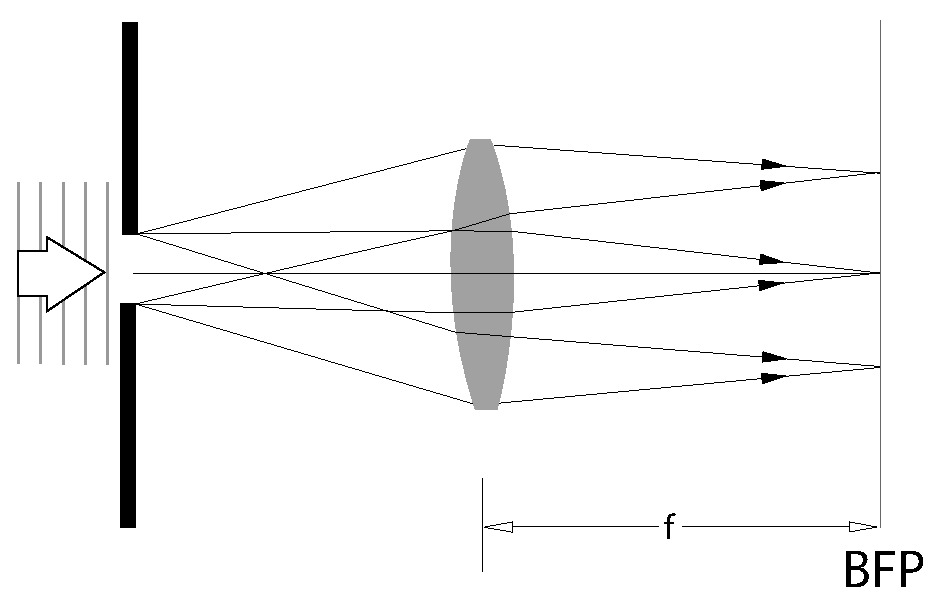
\includegraphics[width=0.5\textwidth]{figures/FourierLinse.pdf}
		\caption{Eine Sammellinse erzeugt das Fraunhofersche-Beugungsbild in ihrer hinteren Brennebene(BFP). Parallele Strahlen werden in Abhängigkeit ihres Winkels zur optischen Achse auf einem Punkt in der BFP fokussiert Die Abbildung ist an \cite{Hecht.2018} angelehnt.}
		\label{fig:FourierLinse}
	\end{figure}
	Da hinter der Probe nicht nur die Leckstrahlung, sondern auch die Strahlung des direkt transmittierten Strahls zu beobachten ist, ist es notwendig, die Leckstrahlung zu selektieren. Die Leckstrahlung tritt dank der notwendigen Phasenanpassung nur unter einem charakteristischen Winkel zur optischen Achse \eqref{eq:phase_condition} aus der Probe aus. Daher ist es möglich, die Leckstrahlung durch ihren Emissionswinkel zu identifizieren. Hierfür ist die Fourier-Optik nützlich. Eine Sammellinse besitzt die Eigenschaft, in  der hinteren Brennebene (BackFocalPlane BFP) ein Winkel aufgelöstes Bild von der Strahlung die sie erreicht, zu erzeugen.\cite{Hecht.1996} Die Position eines Lichtstrahles in der BFP ist also nur von dem Winkel des Strahls zur optischen Achse, nicht aber von der absoluten Position des Strahles vor der Linse abhängig. So ist es möglich gezielt bestimmte Emissionswinkel in der BFP aus dem Bild herauszufiltern. Dieses winkelaufgelöste Bild kann auch als eine räumliche Fouriertransformation der Feldstärkeverteilung an der beobachteten Struktur aufgefasst werden. 
	
	\paragraph{4f-Aufbau}
		In dieser Arbeit wird für diese optische Filterung ein sogenannter 4f Aufbau verwendet. Ein 4f-Aufbau besteht aus zwei Linsen mit der Brennweite $f$, die im Abstand $2f$ zueinander positioniert werden. Die beiden Linsen werden so positioniert, dass sich im Abstand $f$ von der ersten Linse das Zwischenbild des Immersionsobjektives befindet. Zwischen den beiden Linsen entsteht nun ein winkelaufgelöstes Fourierbild. In diesem winkelaufgelöstes Fourierbild kann nun gezielt ein Teil des Formenspektrums (bzw. Strahlung die unter einem bestimmten Winkel zur optischen Achse aus der Probe ausgetreten ist) herausgefiltert werden. Die zweite Linse erzeugt nun aus dem gefiltertem Fourierspektrum wieder das Ortsbild. Dieses besteht nun nur noch aus den gefilterten Fourierkomponenten. Der 4f Aufbau ist schematisch in Abbildung \ref{fig:aufbau_schema} erläutert.
\subsection{Einstellung der Polarisation des Lasers}
		Um den optischen Spin-Hall-Effekt nachweisen zu können, ist es notwendig, die Polarisation des Anregungslasers zu kontrollieren. Hierfür wurde ein Polfilter und eine $\lambda /4$-Verzögerungsplatte verwendet. Der verwendete He-Ne Laser der Firma \textit{Thorlabs} ist linear polarisiert. In Abbildung \ref{fig:polarisationlambda} ist die Polarisation hinter dem Verzögerungsplättchen in Abhängigkeit der relativen Orientierung von Polfilter zu $\lambda /4$-Verzögerungsplättchen dargestellt. 
	\paragraph{Polarisationsfilter}	
		 Um die Polarisationsebene des Lasers präzise festzulegen wurde ein lineare Polfilter verwendet. Ein beliebiger Polarisationszustand lässt sich immer durch eine Überlagerung von zwei senkrecht aufeinander stehenden linearen Polarisationen bilden. Ein Polfilter transmittiert nun nur Licht, dass entlang einer festgelegten Achse linear polarisiert ist. Die anderen Polarisationsrichtungen werden absorbiert oder reflektiert. Ein Polfilter kann also aus einer beliebigen Polarisation linear Polarisierte Licht erzeugen. Der  Polfilter wurde nach dem letzten Spiegel des optischen Aufbaus positioniert, da ein Spiegel im Allgemeinen unterschiedliche Reflektivitäten für Licht, dass senkrecht bzw. parallel zur Einfallsebene des Strahles auf den Spiegel polarisiert ist, aufweist. Der Filter wurde auf eine Polarisation parallel zur Einfallsebene eingestellt und der Laser dann so entlang der optischen Achse gedreht, dass die gemessene Intensität hinter dem Polfilter maximal ist. So entsteht hinter dem Polfilter unabhängig  von der exakten ursprünglichen Polarisation des Lasers p-polarisiertes Licht.
	\paragraph{Verzögerungsplättchen}
		Mit einem Verzögerungsplättchen lässt sich die Polarisation einer einfallenden Welle verändern. Eine EM-Welle lässt sich immer als Überlagerung von zwei linear senkrecht zueinander polarisierten Wellen beschreiben. Diese beiden senkrecht zueinander stehenden Polarisationen sind im allgemeinen zueinander phasenverschoben. Das Funktionsprinzip eines Verzögerungsplättchen ist, die relative Phasenverschiebung zwischen diesen beiden Polarisationen zu verändern. So kann man mit einem geschickt gewählten Verzögerungsplättchen aus jeder beliebigen Ausgangspolarisation in einen beliebigen anderen Polarisationszustand wechseln. Ein Verzögerungsplättchen weist immer eine schnelle und eine langsame Achse auf. Diese beiden Achsen stehen senkrecht aufeinander. Die Phasenverschiebung, die zwischen einer Welle die entlang der langsamen Achse und einer Welle die entlang der schnellen Achse polarisiert ist, auftritt ist eine charakteristische Größe ($\Delta\Phi$) des jeweiligen Verzögerungsplättchens. Physikalische werden Verzögerungsplättchen durch doppelbrechende Kristalle realisiert. Die jeweilige Phasendifferenz ist hierbei von der Dicke des doppelbrechenden Kristalls und dem Brechungsindizes der langsamen und der schnellen Kristallachse abhängig. Wenn das Verzögerungsplättchen so dimensioniert ist, dass die Phasendifferenz zwischen den beiden Polarisationen, die eine EM-Welle beim Durchgang durch das Plättchen erfährt $\Delta \Phi = \pi /4 $ ist, spricht man von einem  $\lambda /4$-Verzögerungsplättchen. Diese Phasendifferenz ist immer auf eine bestimmte Wellenlänge angepasst.  Ein $\lambda /4$-Verzögerungsplättchen kann aus linear polarisiertem Licht zirkular polarisierte Licht erzeugen, wenn eine der beiden Kristallachsen eine Orientierung von 45° zur ursprünglichen Polarisationsachse des Lasers aufweist. Diese Eigenschaft wurde in dieser Arbeit ausgenutzt.
		\begin{figure}
			\centering
			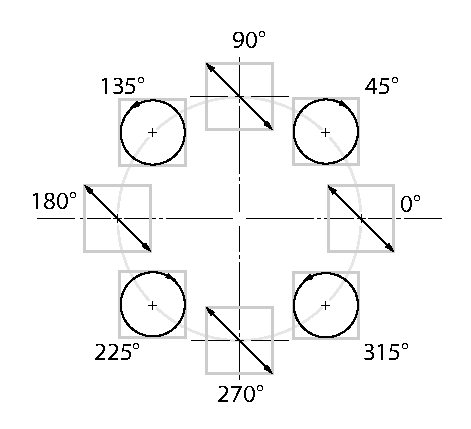
\includegraphics[width=0.5\linewidth]{figures/Polarisation_lambda}
			\caption{Die Abbildung zeigt die Polarisation abhängig von der relativen Orientierung zwischen $\lambda/4$-Plättchen und Polfilter hinter dem $\lambda/4$-Plättchen.}
			\label{fig:polarisationlambda}
		\end{figure}
		
\subsection{Details des optischen Aufbaus}
	In dieser Arbeit wurde der Aufbau von \textit{Jaruschewski} \cite{Jaruschewski.2020} in einigen Details verbessert und umgerüstet, so dass der Laser auch unter schrägen Einfall auf die Probe gerichtet werden kann. Die Verwendeten Komponenten sind detailliert in Anhang \ref{tab:components} aufgelistet. Der Aufbau ist in Abbildung \ref{fig:aufbau_schema} schematisch dargestellt. In dieser Arbeit wurde als Anregungslaser ein He-Ne Dauerstrich Laser der Firma \textit{Thorlabs} mit einer Leistung von $P = 35\mathrm{mw}$ und Wellenlänge $\lambda = 633\mathrm{nm}$ verwendet. Der Laser ist linear polarisiert. Um den CMOS-Detektor vor Beschädigungen zu schützen, wurde ein Neutraldichtefilter verwendet, damit die Leistung des Lasers abgeschwächt werden kann. Um die Fokussierung der Probe zu erleichtern, wurde außerdem eine LED-Hintergrundbeleuchtung verwendet. Das Licht der LED wurde mit einer Sammellinse(f=...) kolimiert, und mit einer weiteren Linse FL $f_{\mathrm{FL}}=50\mathrm{mm}$ auf die  Probe fokussiert. Diese Linse wurde bei Bedarf mit einer Magnetsäule an der richtigen Stelle vor der Probe positioniert.
	\begin{figure}
		\centering
		\begin{subfigure}[b]{0.9\textwidth}		
			\centering
			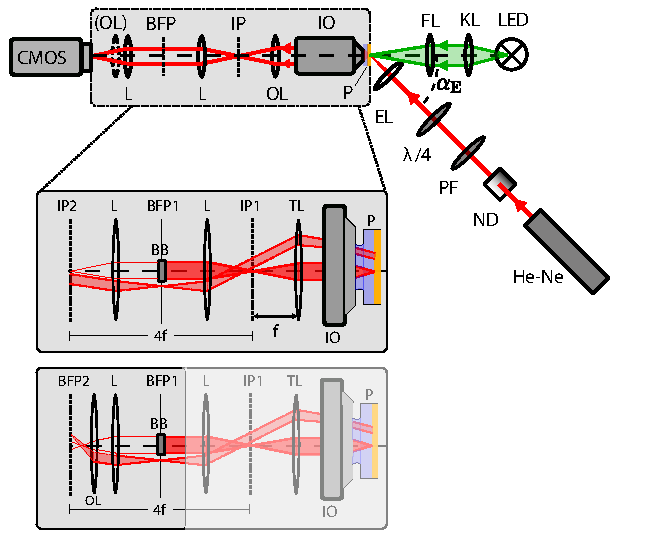
\includegraphics[width=0.9\textwidth]{figures/Aufbau_Schema.pdf}
			\caption{Schematischer Aufbau}			
			\label{fig:aufbau_schema}
		\end{subfigure}
		\vfil
		\begin{subfigure}[b]{0.9\textwidth} 
			\centering
			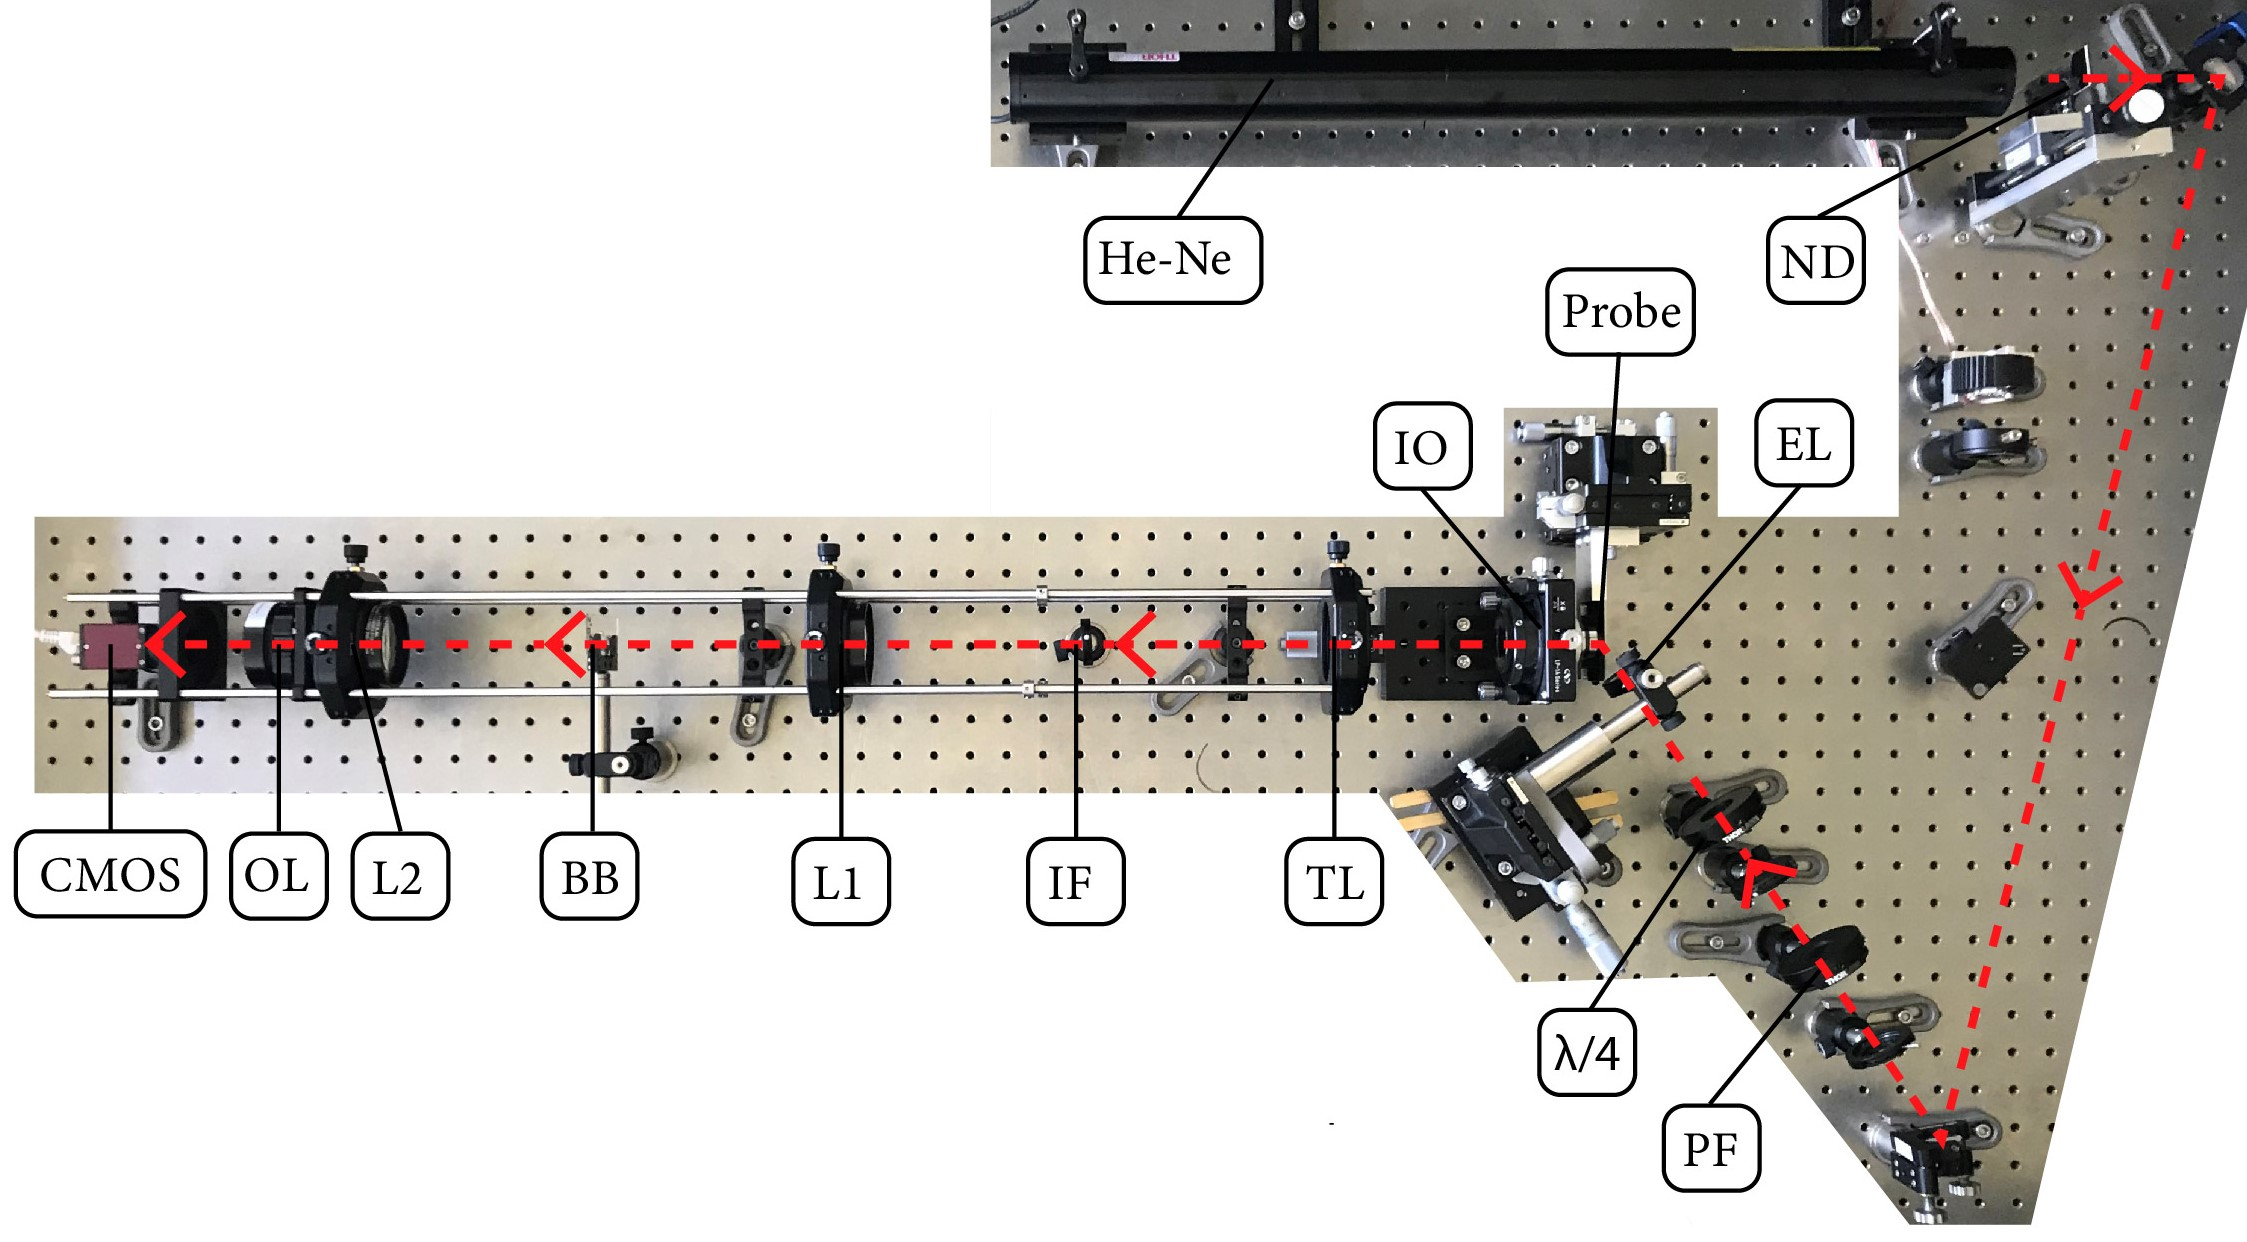
\includegraphics[width=0.9\textwidth]{figures/aufsicht_aufbau_anotated.jpg}
			\caption{Foto des Aufbau}
			\label{fig:aufsicht_aufbau_anotated}
		\end{subfigure}
		\caption{Die Komponenten des Aufbaus sind: CMOS-Sensor (CMOS), Optionale Linse (OL), Linse2 (L2), BeamBlock (BB), Linse1 (L1), ImageFilter (IF), Linse2 (L2), Immersionsobjektiv (IO), Probe, Einkoppel-Linse (EL), Verzögerungsplättchen ($\lambda/4$), Polarisationsfilter (PF), Neutraldichtefilter (ND), He-Ne Laser (He-Ne). Außerdem ist auch noch eine LED Hintergrundbeleuchtung verbaut. In Rot ist schematisch der Strahlengang des Lasers eingezeichnet. Die Abbildung des Schematischen Aufbaus ist an die Abbildung von Jaruschewski \cite{Jaruschewski.2020} angelehnt}
		\label{fig:Aufbau}
	\end{figure}
	\subsubsection{Veränderungen des vorhandenen Aufbaus}
		\paragraph{Einkoppellinse}
		Aus geometrischen Gründen war es nicht mehr möglich, den Laser mit einem Objektiv bei streifenden Einfall auf die Probe zu fokussieren, da sonst das Objektiv mit der Probe kollidieren würde. Stattdessen wurde eine Sammellinse als Einkoppellinse (EL) verwendet mit $f_{\mathrm{EL}}= 30\mathrm{mm}$. Die Wahl der Brennweite der Einkoppellinse ist ein Kompromiss: Je kleiner die Brennweite ist, desto kleiner lässt sich der Laser fokussieren. Wenn die Brennweite allerdings zu klein ist, kollidiert die Linsenhalterung mit der Probe. Mit kleinerer Brennweite sind also nur kleinere Einfallswinkel zur Probennormale möglich. Um trotzdem eine möglichst kleine Brennweite verwenden zu können, wurde eine sehr kompakte Linsenhalterung verwendet. Diese Halterung wurde über einen Querarm an einer xyz-Verfahreinheit montiert, so dass man die Linse in allen drei Raumrichtungen verfahren kann. Dies ist wichtig, um den Laser gezielt auf den Punkt zu fokussieren, an welchem die optische Achse die Probe schneidet. Dieser Aufbau ist in Abbildung \ref{fig:linsenhalterung} gezeigt
		\begin{figure}
			\centering
			\begin{subfigure}[b]{0.4\textwidth}
				\centering
				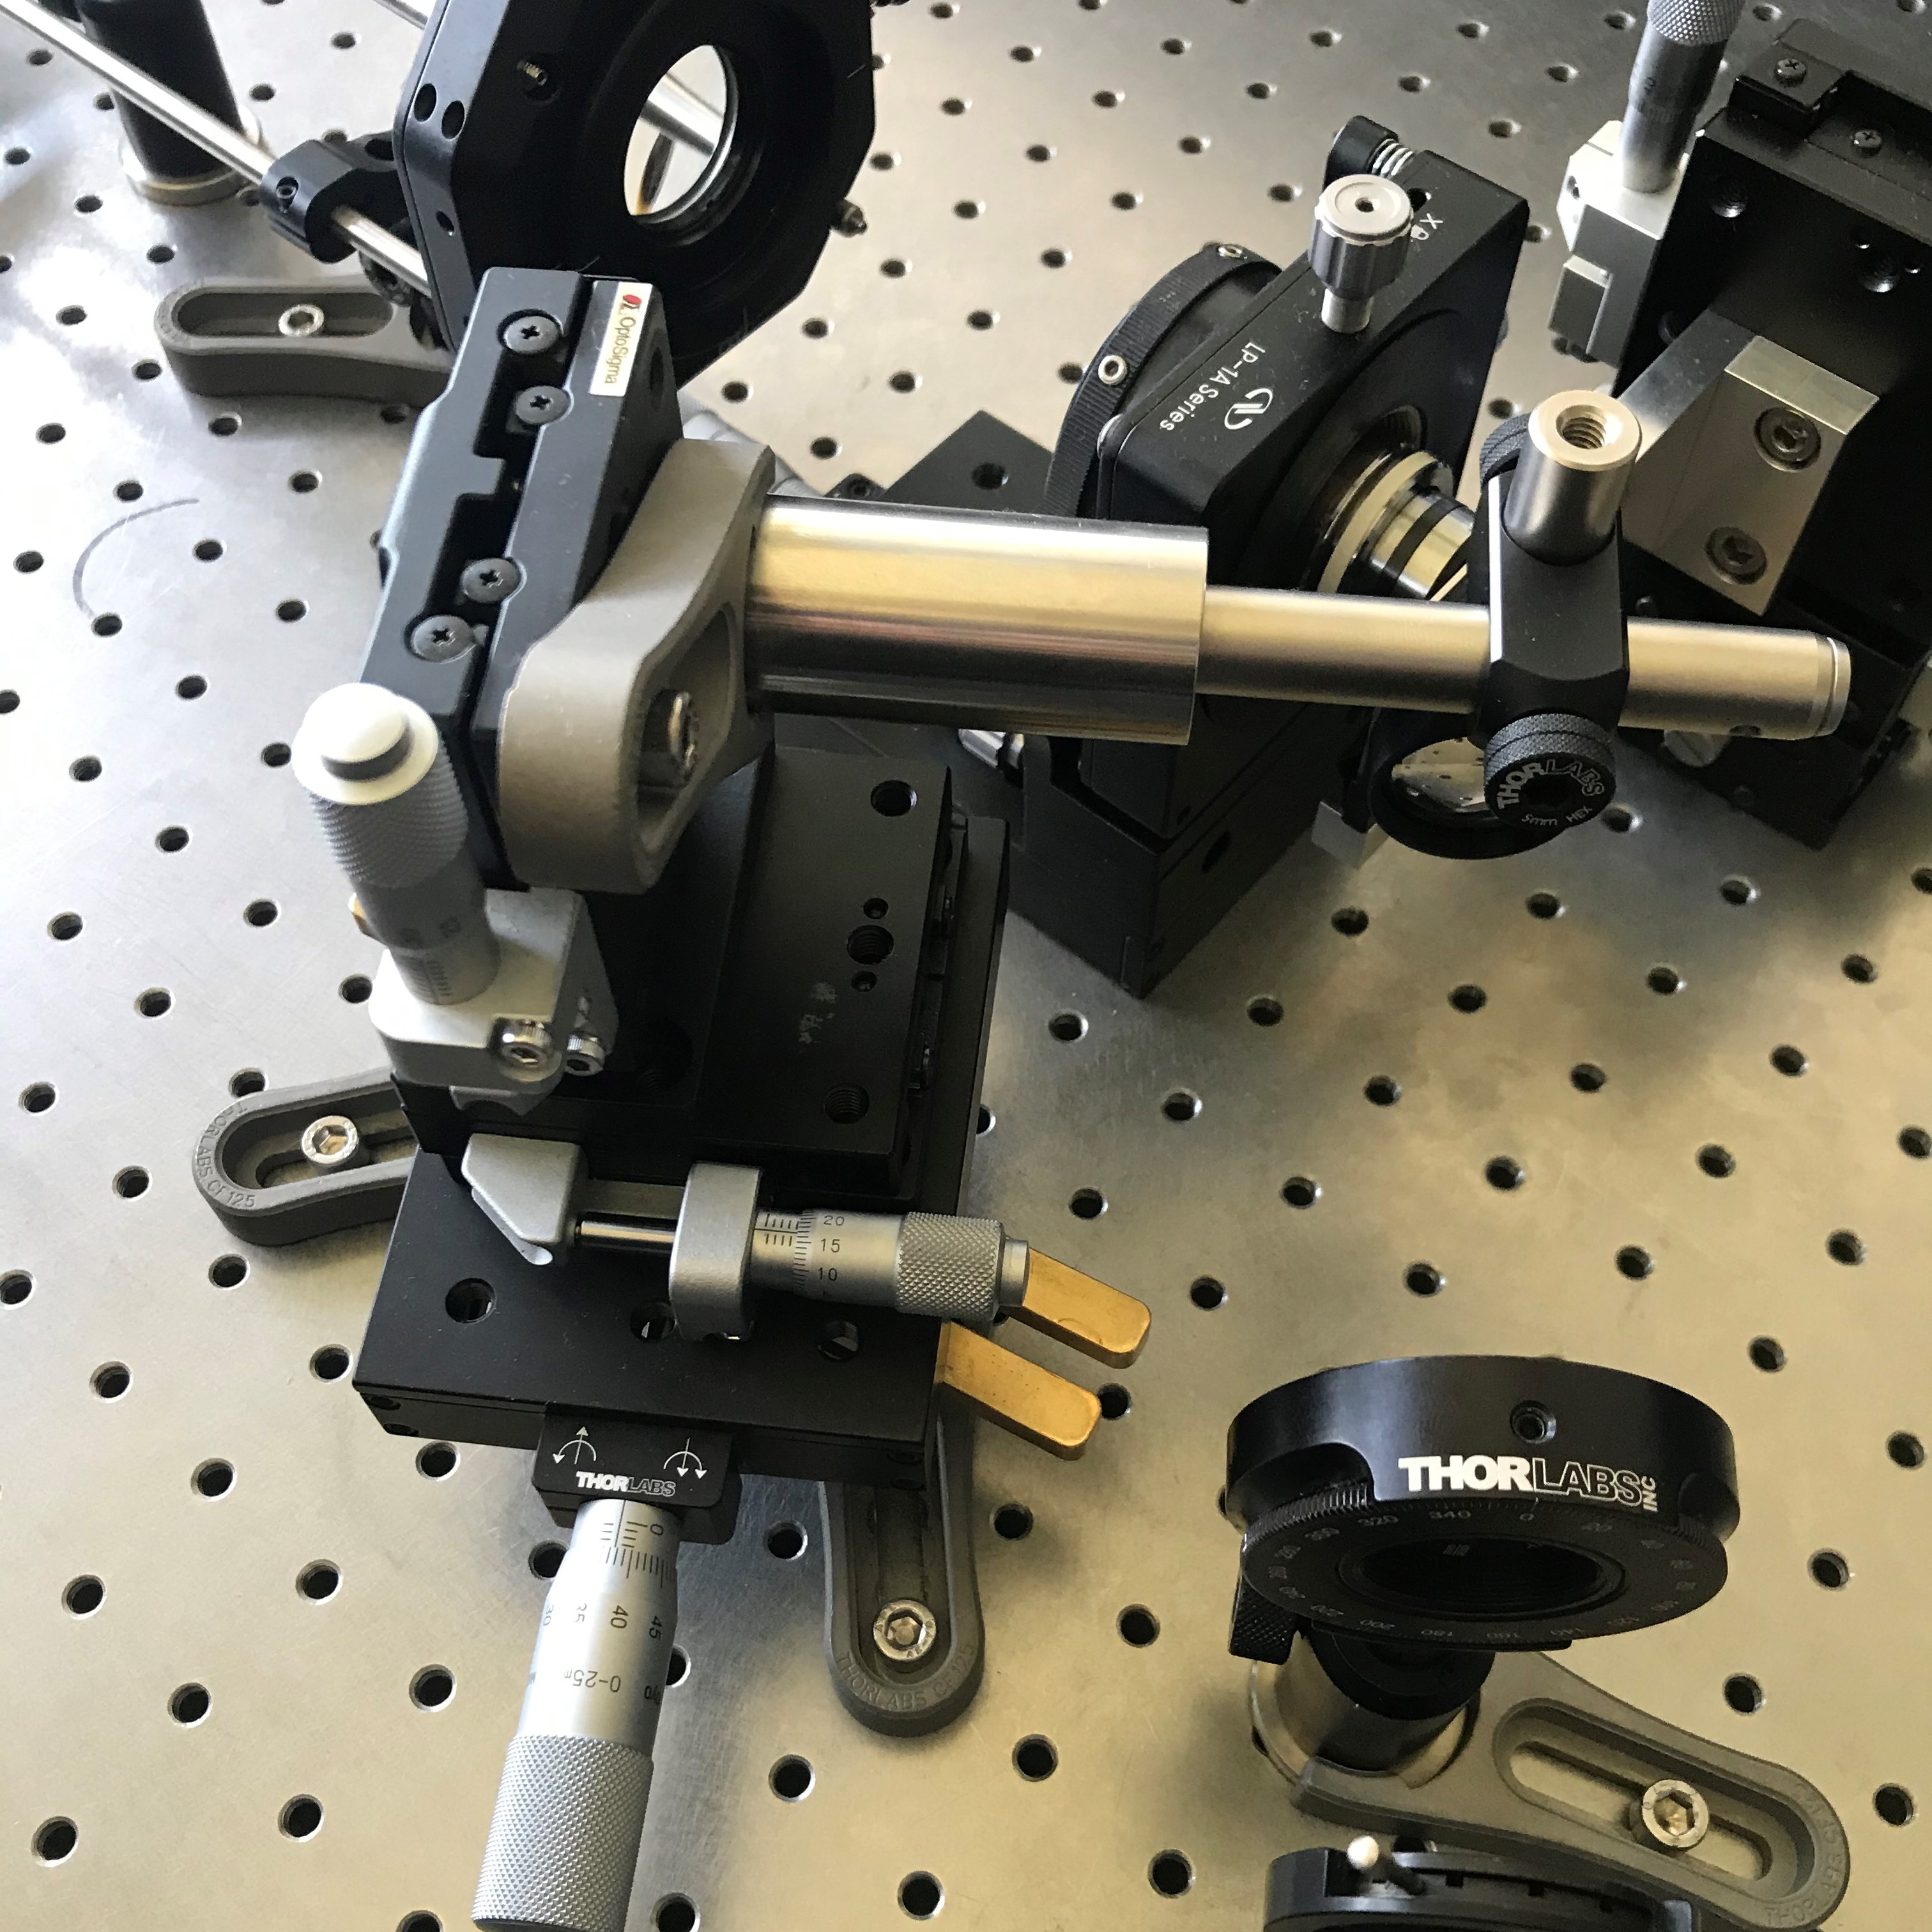
\includegraphics[width=\textwidth]{figures/Einkoppellinse.jpg}
				\caption{Querarm}
				\label{fig:querarm}
			\end{subfigure}
			\hfill
			\begin{subfigure}[b]{0.4\textwidth}
				\centering
				\includegraphics[width=\textwidth]{figures/Kollision_Einkoppellinse.jpg}
				\caption{Kollision Linse mit Probe}
				\label{fig:kollision}
			\end{subfigure}
			\caption{Diese Abbildungen zeigen die Linsenhalterung welche über einen Querarm an einer xyz-Verfahreinheit montiert ist, und die Kollision zwischen Linsenhalterung und Probe}
			\label{fig:linsenhalterung}
		\end{figure}

		\paragraph{Probenhalterung}
			Die Probenhalterung des alten Aufbaus hatte das Problem, dass die senkrechte Ausrichtung der Probe zur Optischen Achse nur grob per Auge erfolgen konnte. Dadurch war beim Verfahren der Probe ein ständiges Nachfokussieren notwendig. Außerdem hatte die Halterung nicht ausreichend Stabilität, was die Fokussierung zusätzlich erschwert hat. Daher wurde im Rahmen dieser Arbeit eine neue Probenhalterung entwickelt. Diese Probenhalterung behebt die Schwachstellen der alten und hat außerdem einen Anschlag für die Probe, so dass es prinzipiell möglich ist, anhand der Skalen an den Mikrometerschrauben der Verfahreinheit Koordinaten abzulesen. So ist es möglich trotz Probenwechsel später wieder die gleichen Orte auf der Probe anzufahren. Die Probenhalterung wurde von der Uni-Werkstatt gefertigt. Eine Technische Zeichnung der Probenhalterung ist im Anhang zu finden.
				\begin{figure}[htbp] 
				\centering
				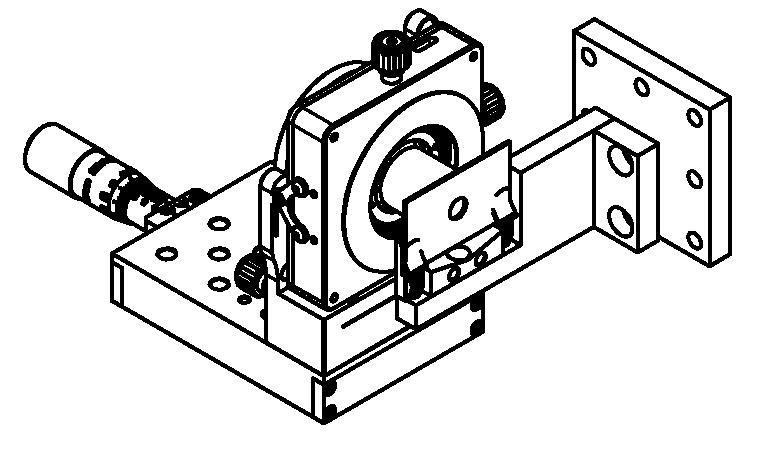
\includegraphics[width=0.5\textwidth]{figures/Probenhalter.pdf}
				\caption{Probenhalter mit Montierter Probe vor dem Immersionsobjektiv}
				\label{fig:probenhalter}
			\end{figure}
		\paragraph{Cage-System}
			Sämtliche Optiken hinter dem Immersionsobjektiv wurden in ein Cage-System der Firma \textit{Thorlabs} integriert (Abbildung \ref{fig:cage_system}). Das Cage-System besteht aus quadratischen Halterungen, die in ihren Eckpunkten Bohrungen habe, durch welche sich Edelstahlstäbe schieben lassen. Diese Fixierung der Halterungen an vier Punkten verhindert ein Verkippen der Linsen entlang der optischen Achse. Die Halterungen können entlang der optischen Achse auf den vier Eckstäben verschoben werden. Für die  Linsen TL, L1, L2 wurden xy-Halter verwendet, die senkrecht zur optischen Achse mit feinen Justierschrauben sehr genau verstellt werden können. Im Laufe dieser Arbeit hat sich herausgestellt, dass diese sehr feine Justierung nicht notwendig gewesen wäre. Die Tubuslinse TL des Herstellers \textit{Zeiss} ist in einem Halter mit einem $M32\times0.5$ Gewinde montiert. Eine Technische Zeichnung der Tubuslinse ist in (...) zu finden. Für dieses Gewinde stellt \textit{Thorlabs} keine Komponenten her, deswegen war ein Adapter notwendig. Eine Technische Zeichnung dieses Adapters ist in (...) zu fingen. Die optionale Linse OL wurde mit einer Magnethalterung in dem Cage-System montiert. Diese Halterung ermöglicht es, die Linse sehr einfach zu entfernen und so zwischen der Darstellung der Image-Plane und Backfocal-Plane zu wechseln. Außerdem wurde die OL in einem längerem Gewindetubus montiert, so das ein präzises Verfahren der Linse entlang der optischen Achse möglich ist. Die ist notwendig, um die BFP präzise zu fokussieren. Ist die richtige Position der OL einmal bestimmt, kann der Gewindetubus mit einem Gewindering gekontert werden. Auch der CMOS-Sensor der Firma \textit{Alllied-Vision} wurde in das Cage-System integriert. Hierfür war ein Adapter von der Kameraobjektiv-Gewindenorm \textit{C-Mount} auf die Gewindenorm \textit{SM-2} des Cage-System Herstellers \textit{Thorlabs} notwendig. Ein Technische Zeichnung des Cage-Systems ist im Anhang (...) zu finden. Der BeamBlock (BB) und der ImageFilter (IF) sind mit Magnetsäulen auf dem optischen Tisch befestigt.
			\begin{figure}[htbp] 
				\centering
				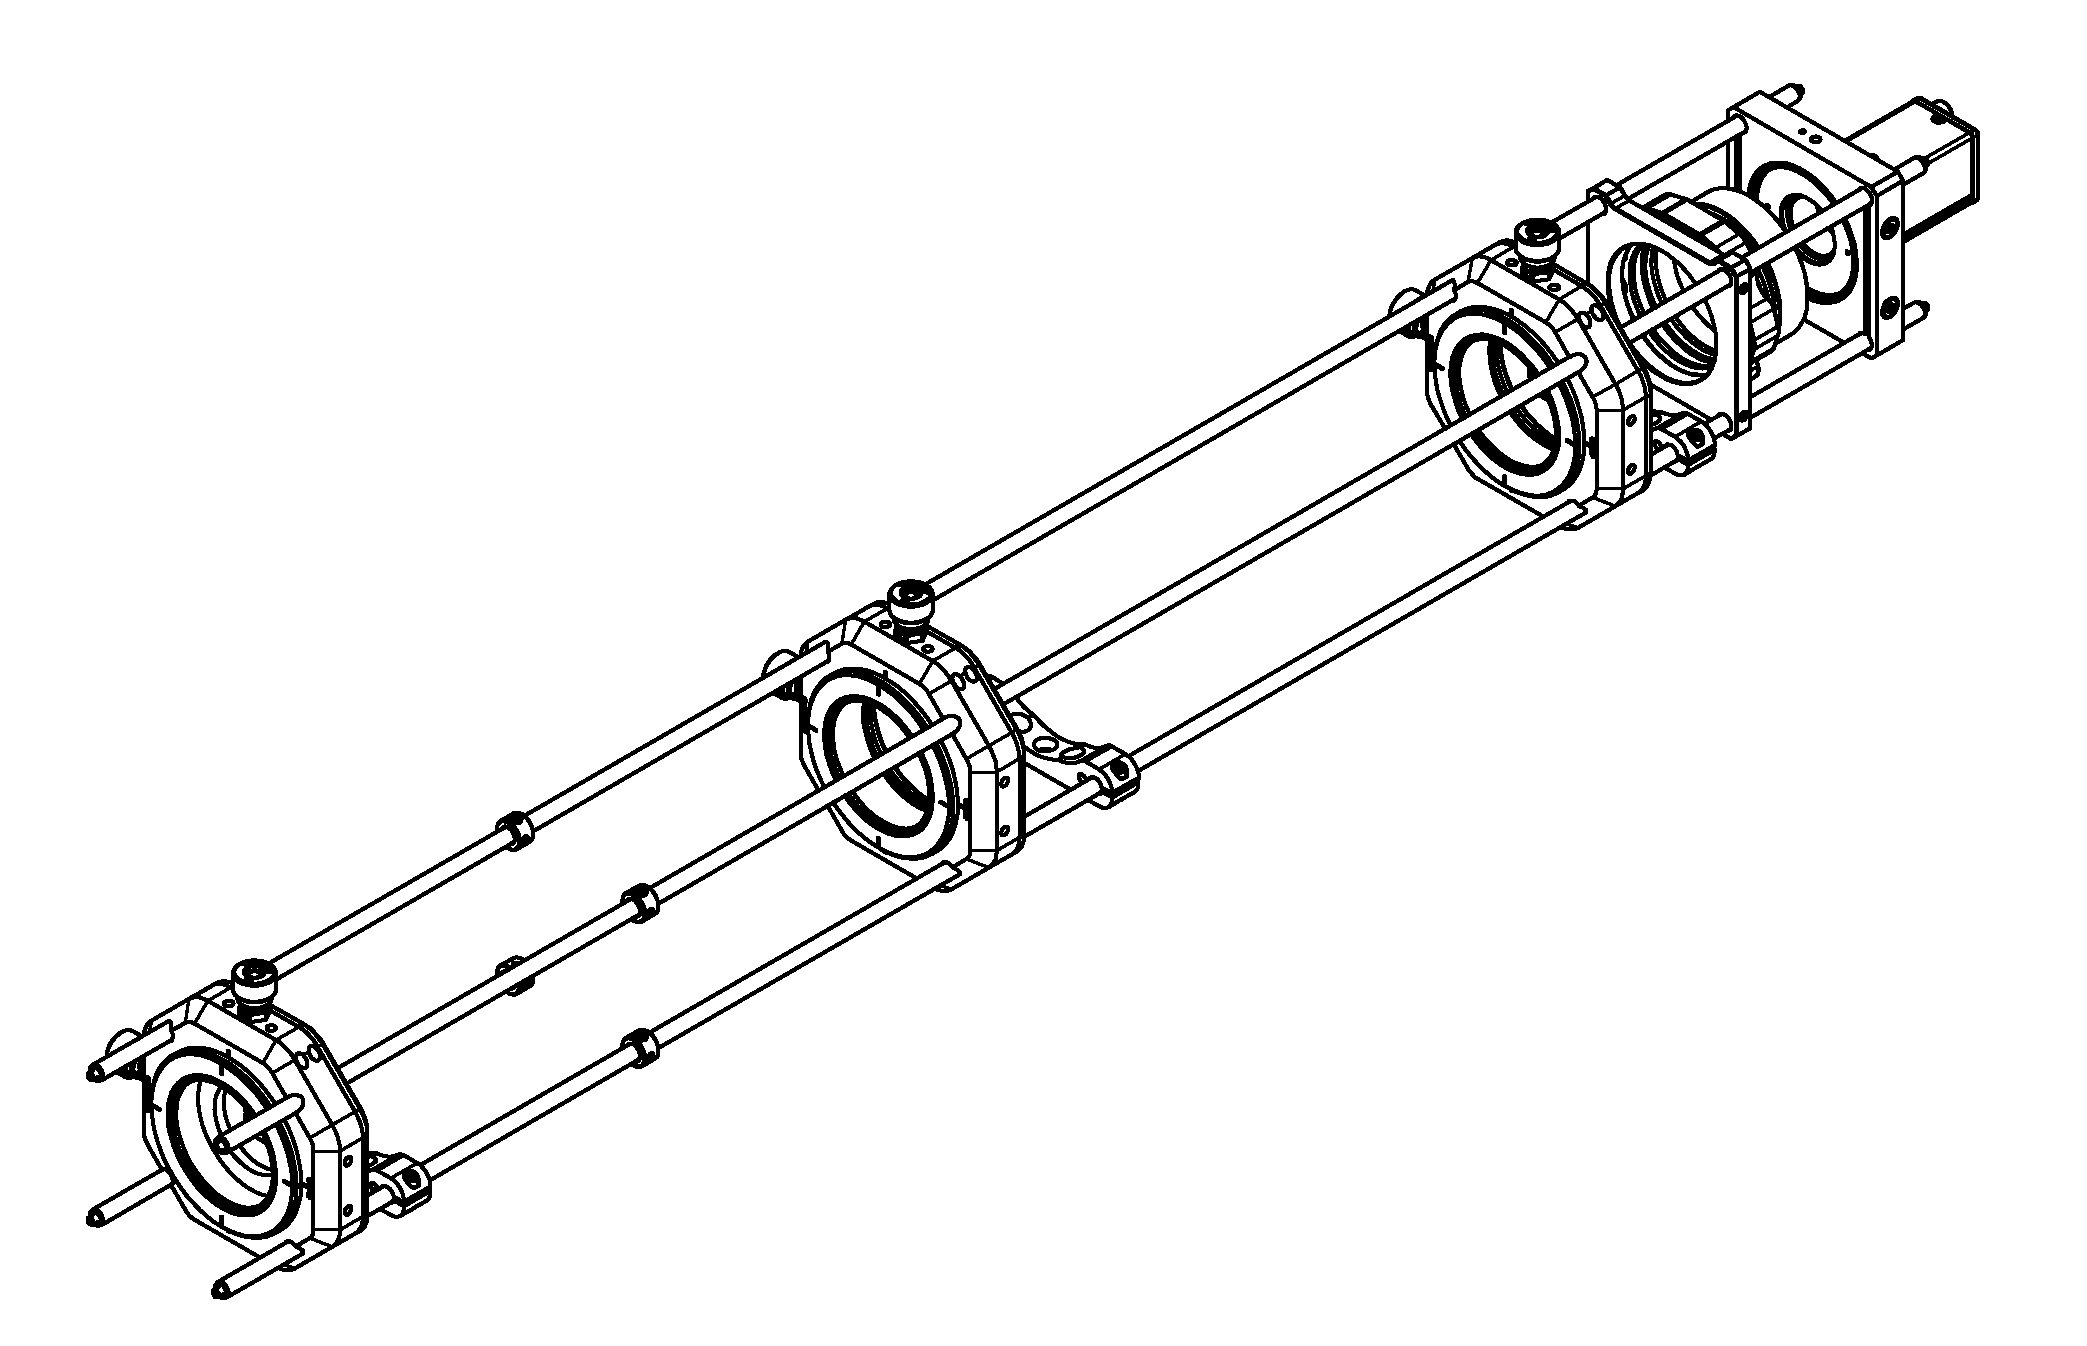
\includegraphics[width=0.7\textwidth]{figures/Cage_System.pdf}
				\caption{Tubuslinse, 4f-System, optionale Linse und CMOS im Cage-System}
				\label{fig:cage_system}
			\end{figure}	
\subsection{Probe}
	Die ersten Messungen dieser Arbeit wurden mit Proben, die noch durch die Messungen von Jaruschewski \cite{Jaruschewski.2020} vorhanden waren durchgeführt. Da diese Proben jedoch auch auf der Goldseite mit Imersionsöl verdreckt waren, wurden später neue Proben verwendet, diese Proben wurden von Till Leißner in Sonderborg hergestellt. Hierfür wurden Deckgläser der Firma \textit{Carl Zeiss} mit einem Brechungsindex von $n_{\mathrm{Glas}}= 1.52$ verwendet. Die Deckgläser wurden mit einer $d_{\mathrm{Gold}} = 50\mathrm{nm}$ dicken Goldschicht bedampft. Die Deckgläser haben eine Dicke von $d_{\mathrm{Glas}} = 170 \mathrm{\mu m}$. Als Anregungsstruktur wurden Defektstellen verwendet. Die Proben wurden in kleine Edelstahlbleche (Technische Zeichnung \ref{fig:tz_probenblech}) eingeklebt, welche wiederum in die Probenhalterung passen. Damit die Proben auf der Goldseite nicht mit Immersionsöl verdreckt werden, wurden die sie mit einem Epoxid-Kleber in die Edelstahlbleche eingeklebt.
	\begin{figure}
		\centering
		\begin{subfigure}[b]{0.4\textwidth}
			\centering
			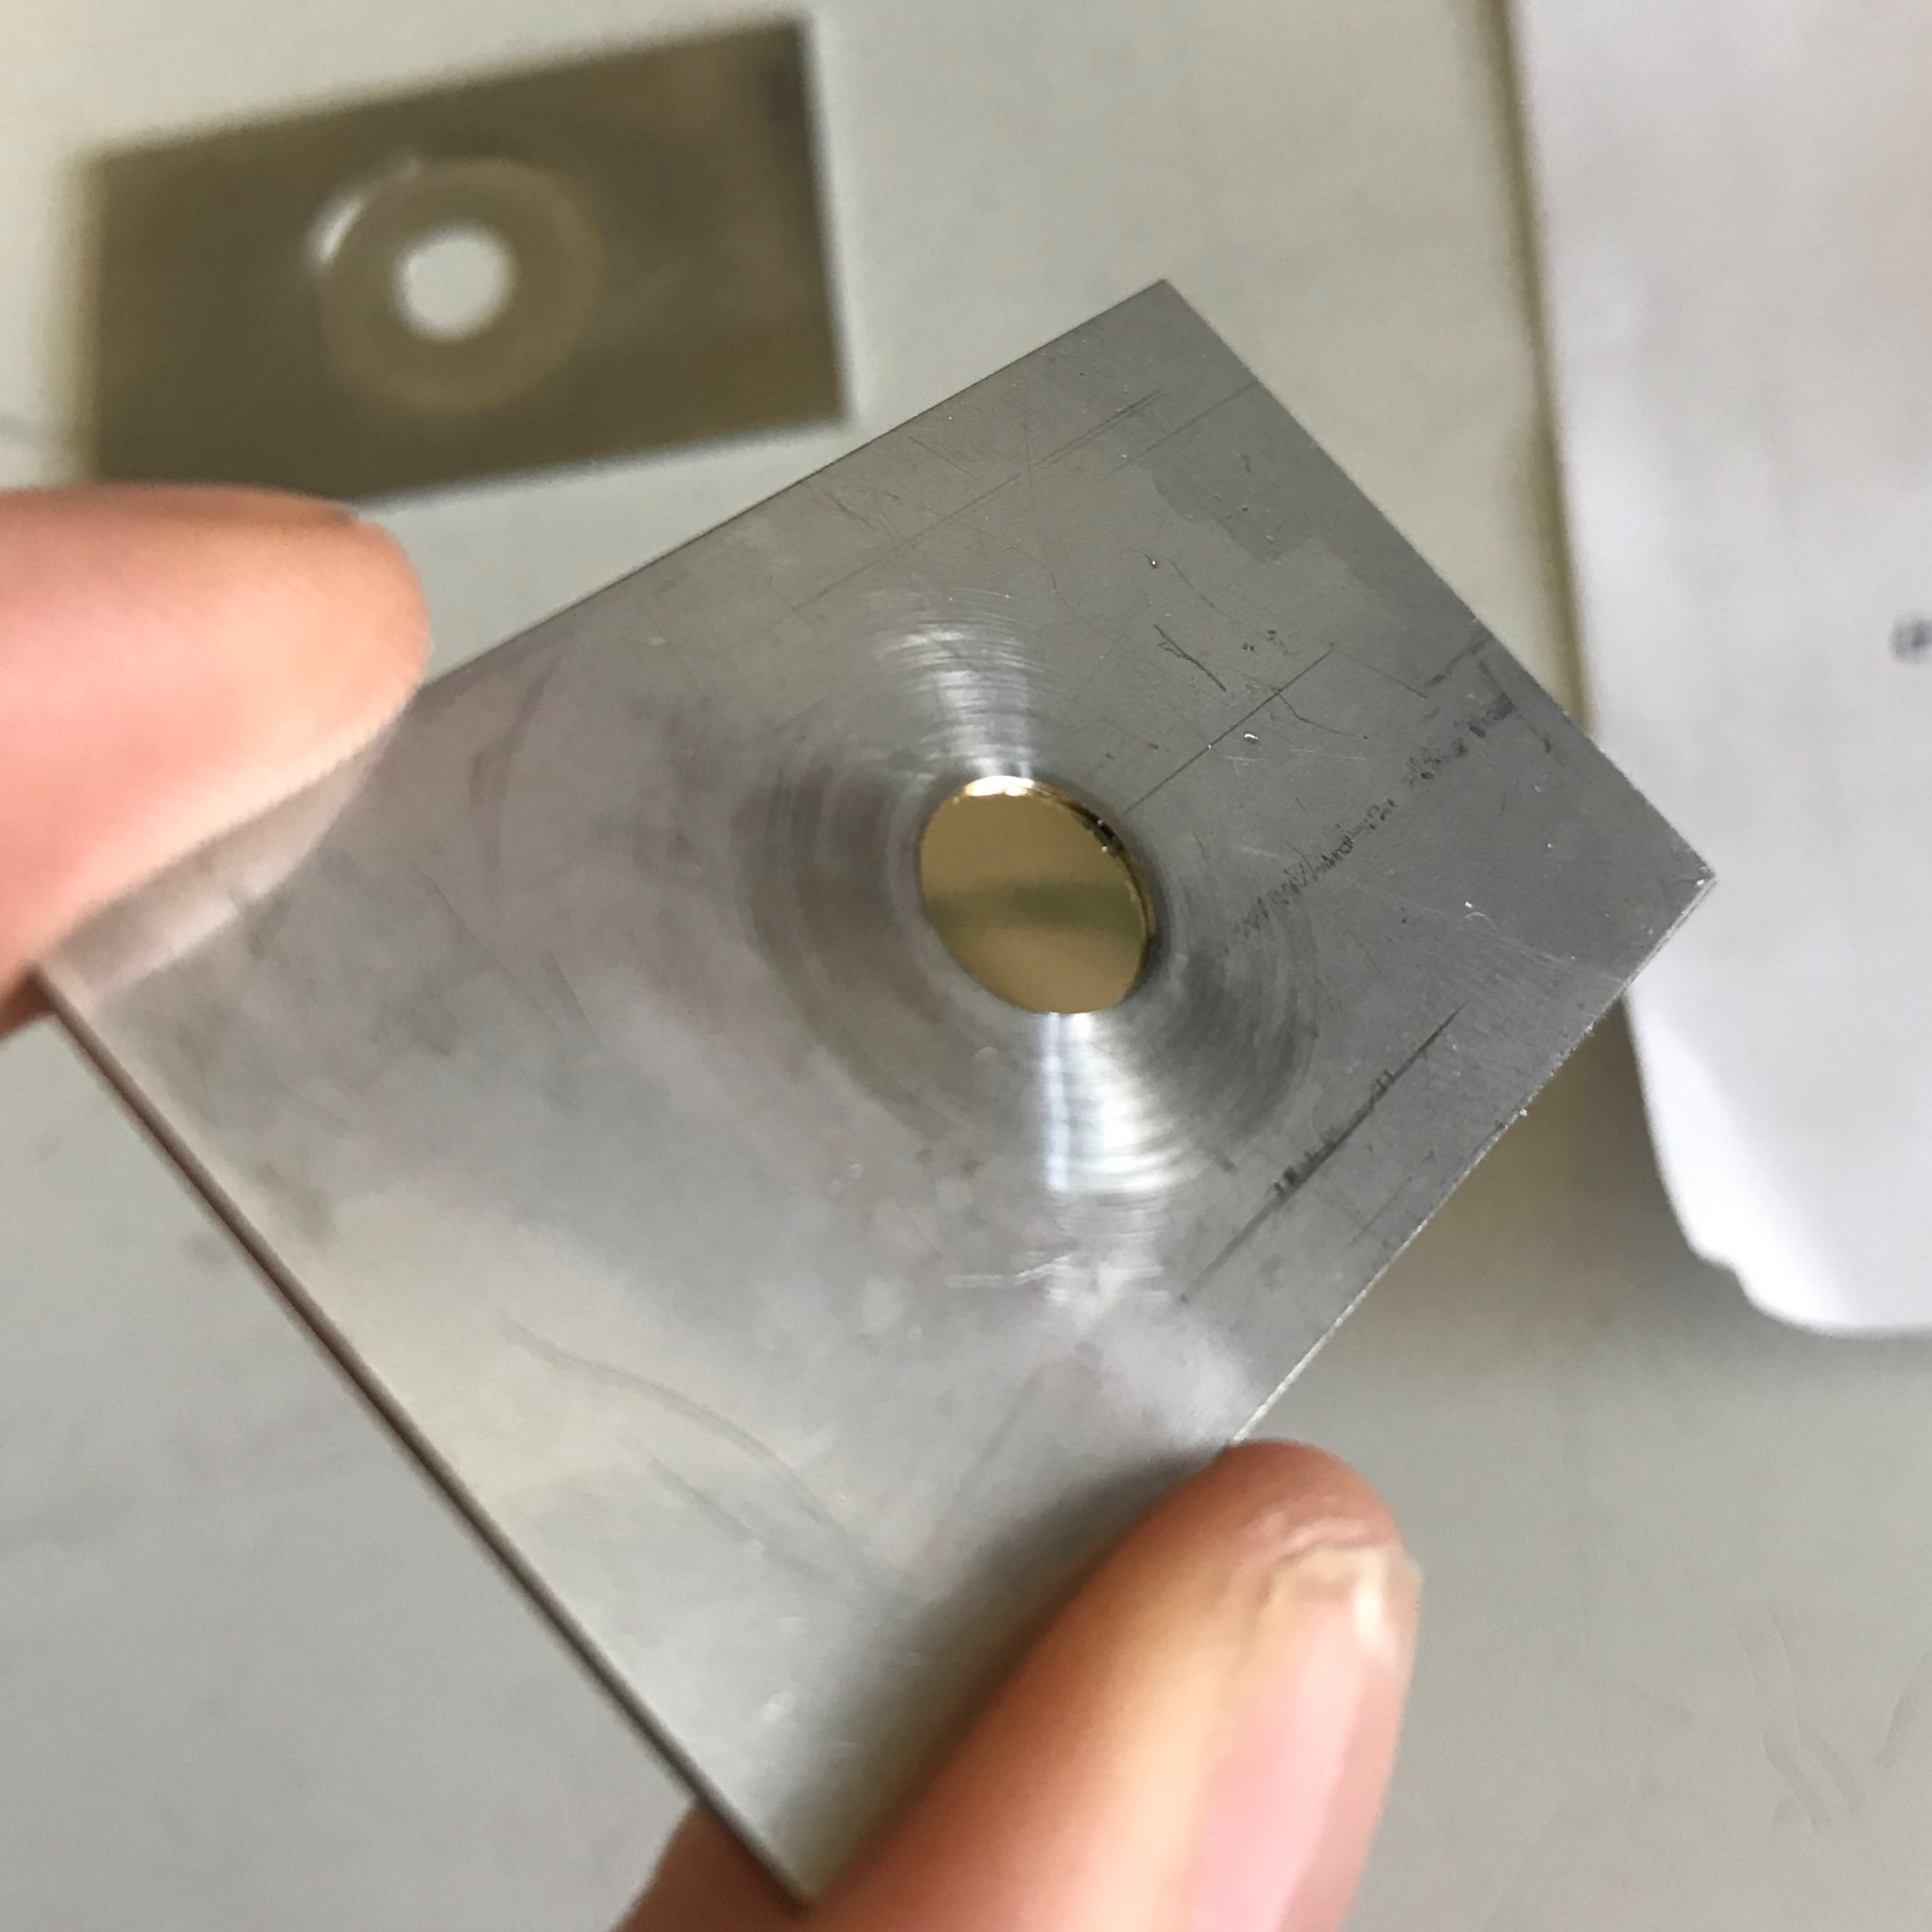
\includegraphics[width=\textwidth]{figures/Probe_Vorderseite.jpg}
			\caption{Goldseite}
			\label{fig:probe_vorderseite}
		\end{subfigure}
		\hfill
		\begin{subfigure}[b]{0.4\textwidth}
			\centering
			\includegraphics[width=\textwidth]{figures/Probe_Rueckseite.jpg}
			\caption{Glasseite}
			\label{fig:probe_rueckseite}
		\end{subfigure}
		\caption{Die Bilder zeigen die in das Edelstahlblech eingeklebte Probe. In rot ist die Verklebung markiert. Hierbei ist darauf zu achten, dass die Klebung dicht ist, so dass kein Öl von der Glasseite auf die Goldseite laufen kann.}
		\label{fig:probe}
	\end{figure}
\subsection{Justage des Aufbaus}
Die allgemeine Justage des LRM verlief, bis auf das Justieren des Lasers auf die Probe, wie von Jaruschewski \cite{Jaruschewski.2020} beschrieben. Dieses war durch den notwendigen schrägen Einfall des Lasers auf die Probe deutlich erschwert. Die Justage erfolgte mit montierter Probe. Als erste wurde die Probe mit Hilfe der Hintergrundbeleuchtung in den korrekten Abstand zum IO gebracht(Im korrekten Abstand ist das Bild der Probe scharf zu sehen). Als nächstes wurde der Laser mit zwei Spiegeln grob in dem erwünschten Winkel auf die Probe justiert. Danach wurden Einkoppellinse, $\lambda/4$-Plättchen und Polfilter in den Strahlgang gestellt. Die Feinjustierung des Lasers auf die Probe wurde nun durch das Verschieben der Einkoppellinse durchgeführt. Hierbei war es hilfreich, den Strahl durch das Verfahren der EL entlang der optischen Achse etwas zu de-fokussieren, so dass man die Randbereiche des Strahls über den CMOS-Sensor in der Image-Plane auch schon sehen kann, wenn der Strahl noch nicht exakt die optische Achse trifft. Sobald ein Teil des Strahles in der Image-Plane detektiert worden ist, wird er durch weiteres bewegen der Linse zentriert und dann sukzessive weiter fokussiert. Durch das Verkippen der Einkoppellinse zum Laser, wandert der Strahl beim Fokussieren des Lasers stark auf der Probe. Das Verkippen der Linse wird, sobald der Laser optimal fokussiert ist, behoben. Hierfür wird der Laser durch die beiden Spiegel sukzessive so einjustiert, dass der Spot auf der Probe beim de-fokussieren des Lasers nicht mehr wandert. 
\subsection{Messung}
Zunächst wurde die Funktionsfähigkeit des LRM durch einige Probe-Messungen, die mit den Daten von Jaruschewski \cite{Jaruschewski.2020} und Ebel \cite{ebel.2019} verglichen worden ist, überprüft. Da für den Nachweis des Plasmonischen-Spin-Hall-Effektes keine Kenntnisse über den Betrag des Wellenvektors notwendig ist, wurde auf eine Kalibrierung der BFP verzichtet. Die in den Abbildungen dargestellten Skalen von $|\vec{k}_{\mathrm{SPP}}|$ wurden durch die bekannte Luft-Gold Mode berechnet. Die Polarisation des Lasers wurde so ausgerichtet, dass sie bei Orientierung des $\lambda/4$-Plättchen $\alpha_{\lambda/4} \in \{0^\circ, 90^\circ, 180^\circ, 270^\circ\}$ parallel zur Einfallsebene des Lasers liegt.  Dann wurde ein geeigneter Defekt auf der Probenoberfläche gesucht. Das Vorgehen hierbei war, die Probe zu verfahren und dabei das Bild der BFP zu beobachten. Sobald der Laser hierbei auf einen Defekt trifft, sind in der BFP die charakteristischen Fringes der Leckstrahlung zu erkennen. Das Ziel war es, einen Defekt zu finden, der möglichst symmetrisch abstrahlt. Nach dem ein geeigneter Defekt gefunden worden ist, wurden Bilder der FP und der BFP für unterschiedliche Orientierungen des $\lambda/4$-Plättchen bei gleichbleibender Belichtungszeit aufgenommen.

\section{Ergebnisse und Diskussion}
	\subsection{Überprüfung der Funktionsweise des LRM}
		In diesem Abschnitt soll kurz verifiziert werden, ob die Messdaten des LRM tatsächlich Plasmonischer Natur sind. Dafür wurden die Anregung an einem Punktdefekt bei einem Einfallswinkel $\alpha_{\mathrm{E}} = 60^\circ$ bei linearer Polarisation parallel zur Einfallsebene untersucht. Da die Begrenzung der BFP durch die NA nur vom Imersionsobjektiv und dem Brechungsindex des verwendeten Immersionsöls abhängt, ist diese Begrenzung gut geeignet, um eine Kalibrierung der BFP zu ermöglichen. In dieser Arbeit wird sowohl das gleiche Immersionsöl als auch das gleiche Immersionsobjektiv wie in\cite{Jaruschewski.2020} verwendet. Daher kann die Kalibrierung aus dieser Arbeit übernommen werden. Dort wurde durch eine SPP-Mode mit bekanntem $k_{\mathrm{spp}}$ der Wert der Numerischen Apertur der Kombination Immersionsobjektiv-Immersionsöl bei einer Wellenlänge von $\lambda=633\mathrm{nm}$ auf $\mathrm{NA}_{\lambda = 633 \mathrm{nm}} = 1.216 \pm 0.005$  und $k_0\mathrm{NA}_{\lambda = 633 \mathrm{nm}} = 12.07 \pm 0.05\mathrm{\mu m}^{-1}$ bestimmt. Anhand dieser Kalibrierung wurde der Wert von $k_{\mathrm{spp}}$ bestimmt. Hierfür wurde für jeden Radius das Integral:
		$$ I\left(|\vec{k}_{\bot}|\right) = \int_{0}^{2 \pi} I\left(|\vec{k}_{\bot}|, \theta\right)\mathrm{d}\theta$$
		ausgewertet. Das Maximum dieser radialen Intensitätsverteilung entspricht $k_{\mathrm{spp}} = 10.35\mathrm{\mu m}^{-1}$.
		 Dieser Wert stimmt bis auf $0.2\%$ mit dem Wert aus der theoretischen Berechnung \eqref{eq:theo_k_spp} überein. Allerdings ist hier zu bemerken, dass die Luft-Gold-Glas Mode auch für die Kalibrierung genutzt worden ist. Die Messdaten sind in Abbildung \ref{fig:example_bfp} und die radiale Intensitätsverteilung ist in Abbildung \ref{fig:radial_profile} dargestellt. Die Einfallsrichtung des Lasers war entlang der $0^\circ$-Linie. Es fällt auf, dass die Anregung in Richtung der Einfallsebene deutlich stärker ausgeprägt ist. 
			\begin{figure}
				\label{fig:example_measure}
				\centering
				\begin{subfigure}[b]{0.5\textwidth}
					\centering
					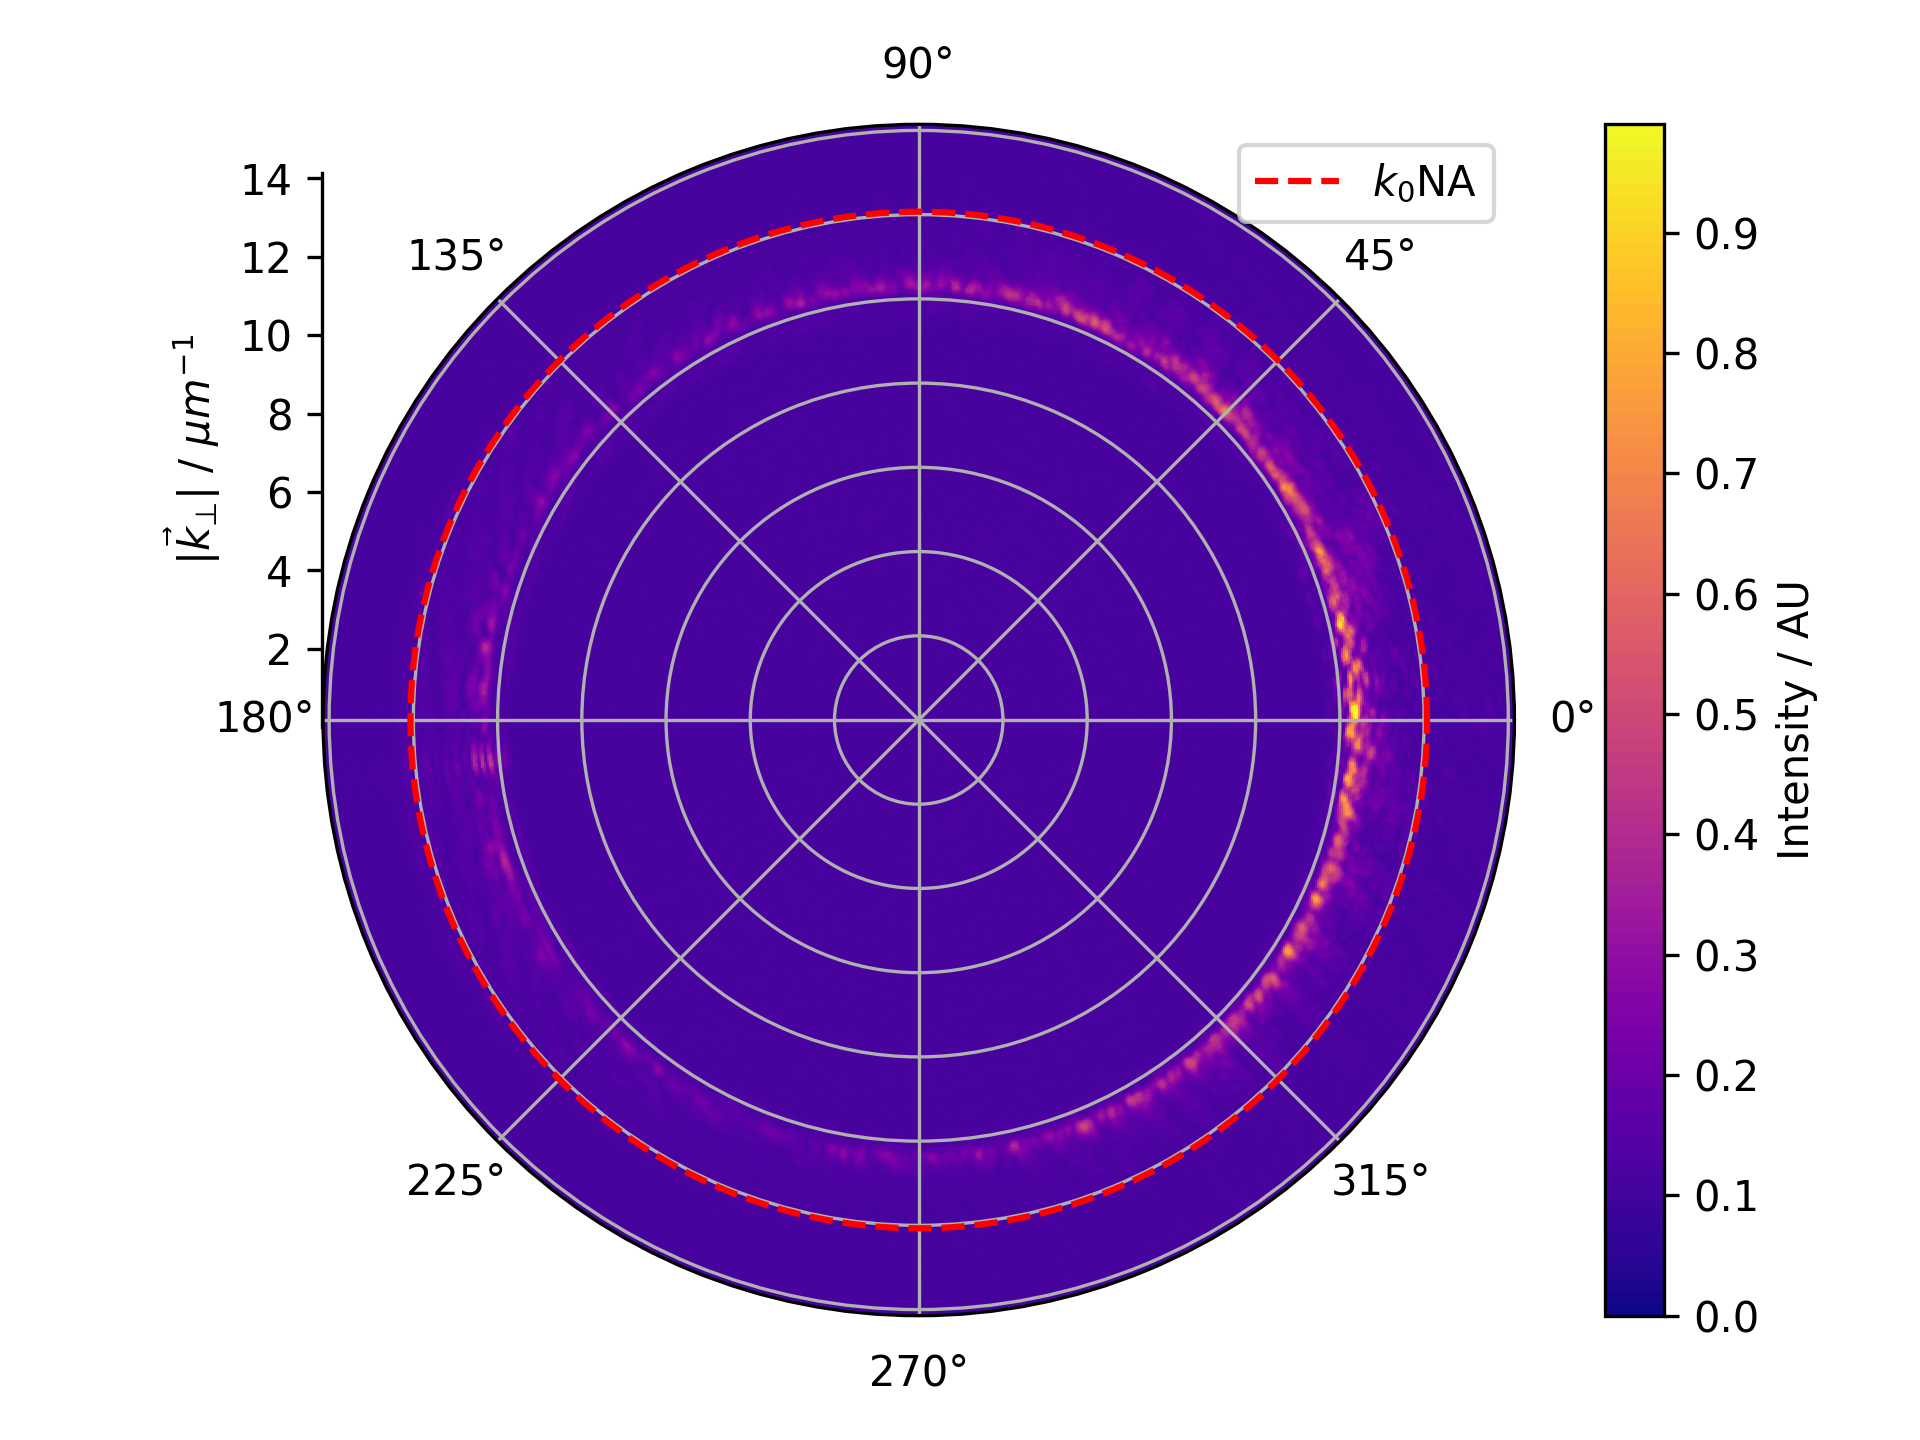
\includegraphics[width=\textwidth]{figures/example_polar.png}
					\caption{Intensitätsverteilung in der BFP}
					\label{fig:example_bfp}
				\end{subfigure}
				\hfill
				\begin{subfigure}[b]{0.49\textwidth}
					\centering
					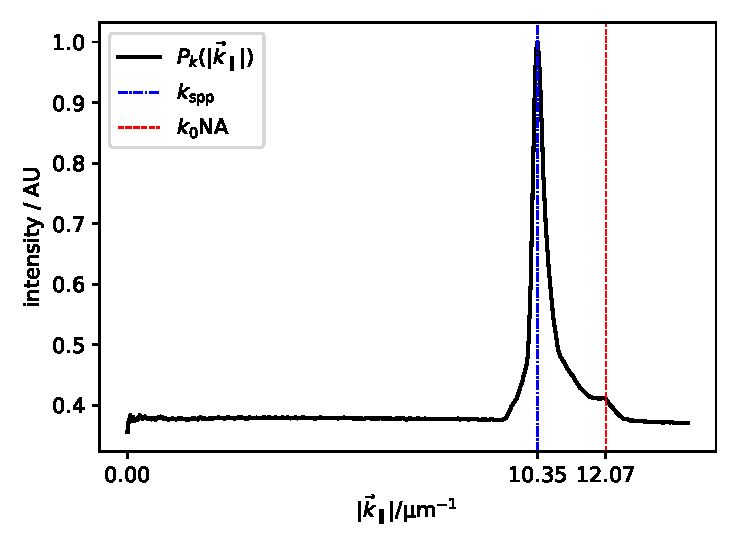
\includegraphics[width=\textwidth]{figures/example_radial.pdf}
					\caption{Radiale Intensitätsverteilung in der BFP}
					\label{fig:radial_profile}
				\end{subfigure}
				\caption{ Messung unter $\alpha_{\mathrm{E}} = 60^\circ$ bei p-Polarisation.
					Der rot markierte Knick in der Intensitätsverteilung entsteht durch die Begrenzung der BFP durch die NA und wurde ausgenutzt, um die Skala zu kalibrieren. Die radiale Intensitätsverteilung hat ein Maximum bei $k_{\mathrm{spp}}= 10.35 \mathrm{\mu m ^{-1}}$.}			
			\end{figure}
	\subsection{Nachweis des Plasmonischen Spin-Hall-Effektes}
	Zum Nachweis des Plasmonischen Spin-Hall-Effektes wurde das plasmonische k-Spektrum an einem Punktdefekt in Abhängigkeit der Orientierung des $\lambda /4$-Plättchens gemessen. Die Messung wurde an einem Punktdefekt durchgeführt. Bei der Auswahl des Defektes wurde auf eine möglichst isotrope Anregung und eine möglichst Defekt freie Umgebung geachtet. Das Ortsbild wurde in der Imageplane 1 mit einer Blende auf auf einen einzelnen Defekt gefiltert. Es wurde die BFP für in Unterschiedliche Orientierungen des $\lambda/4$-Plättchens von $0^\circ-360^\circ$ mit einer Schrittweite von $2^\circ$ aufgenommen. Außerdem wurde mit einer Schrittweite von $20^\circ$ das Ortsbild der Anregung aufgenommen.
	
	Die so entstandenen Bilder der BFP wurden mit einem Python-Script ausgewertet. Hierfür wurde das kartesische Pixel-Bild zunächst in Polarkoordinaten Transformiert. Hierbei fand eine Interpolation der Daten auf ein äquidistantes Gitter in Polarkoordinaten statt. In der BFP wurden nun senkrecht zur Einfallsebene des Lasers zwei Integrationsbereiche ausgewählt. Im nächsten Schritt wurde für jede Orientierung des $\lambda/4$-Plättchens das Kontrastverhältnis der beiden Integrationsbereiche berechnet. Diese Kontrastverhältnisse zeigen die Abhängigkeit der Propagations-Richtung des SPPs von der Polarisation des Anregenden-Lasers. Diese Daten sind in Abbildung \ref{fig:diff_back} - \ref{fig:intensity_front} für unterschiedliche Integrationsbereiche dargestellt.
	\begin{figure}
		\label{fig:spin_hall_measure}
		\centering
		\begin{subfigure}[b]{0.5\textwidth}
			\centering
			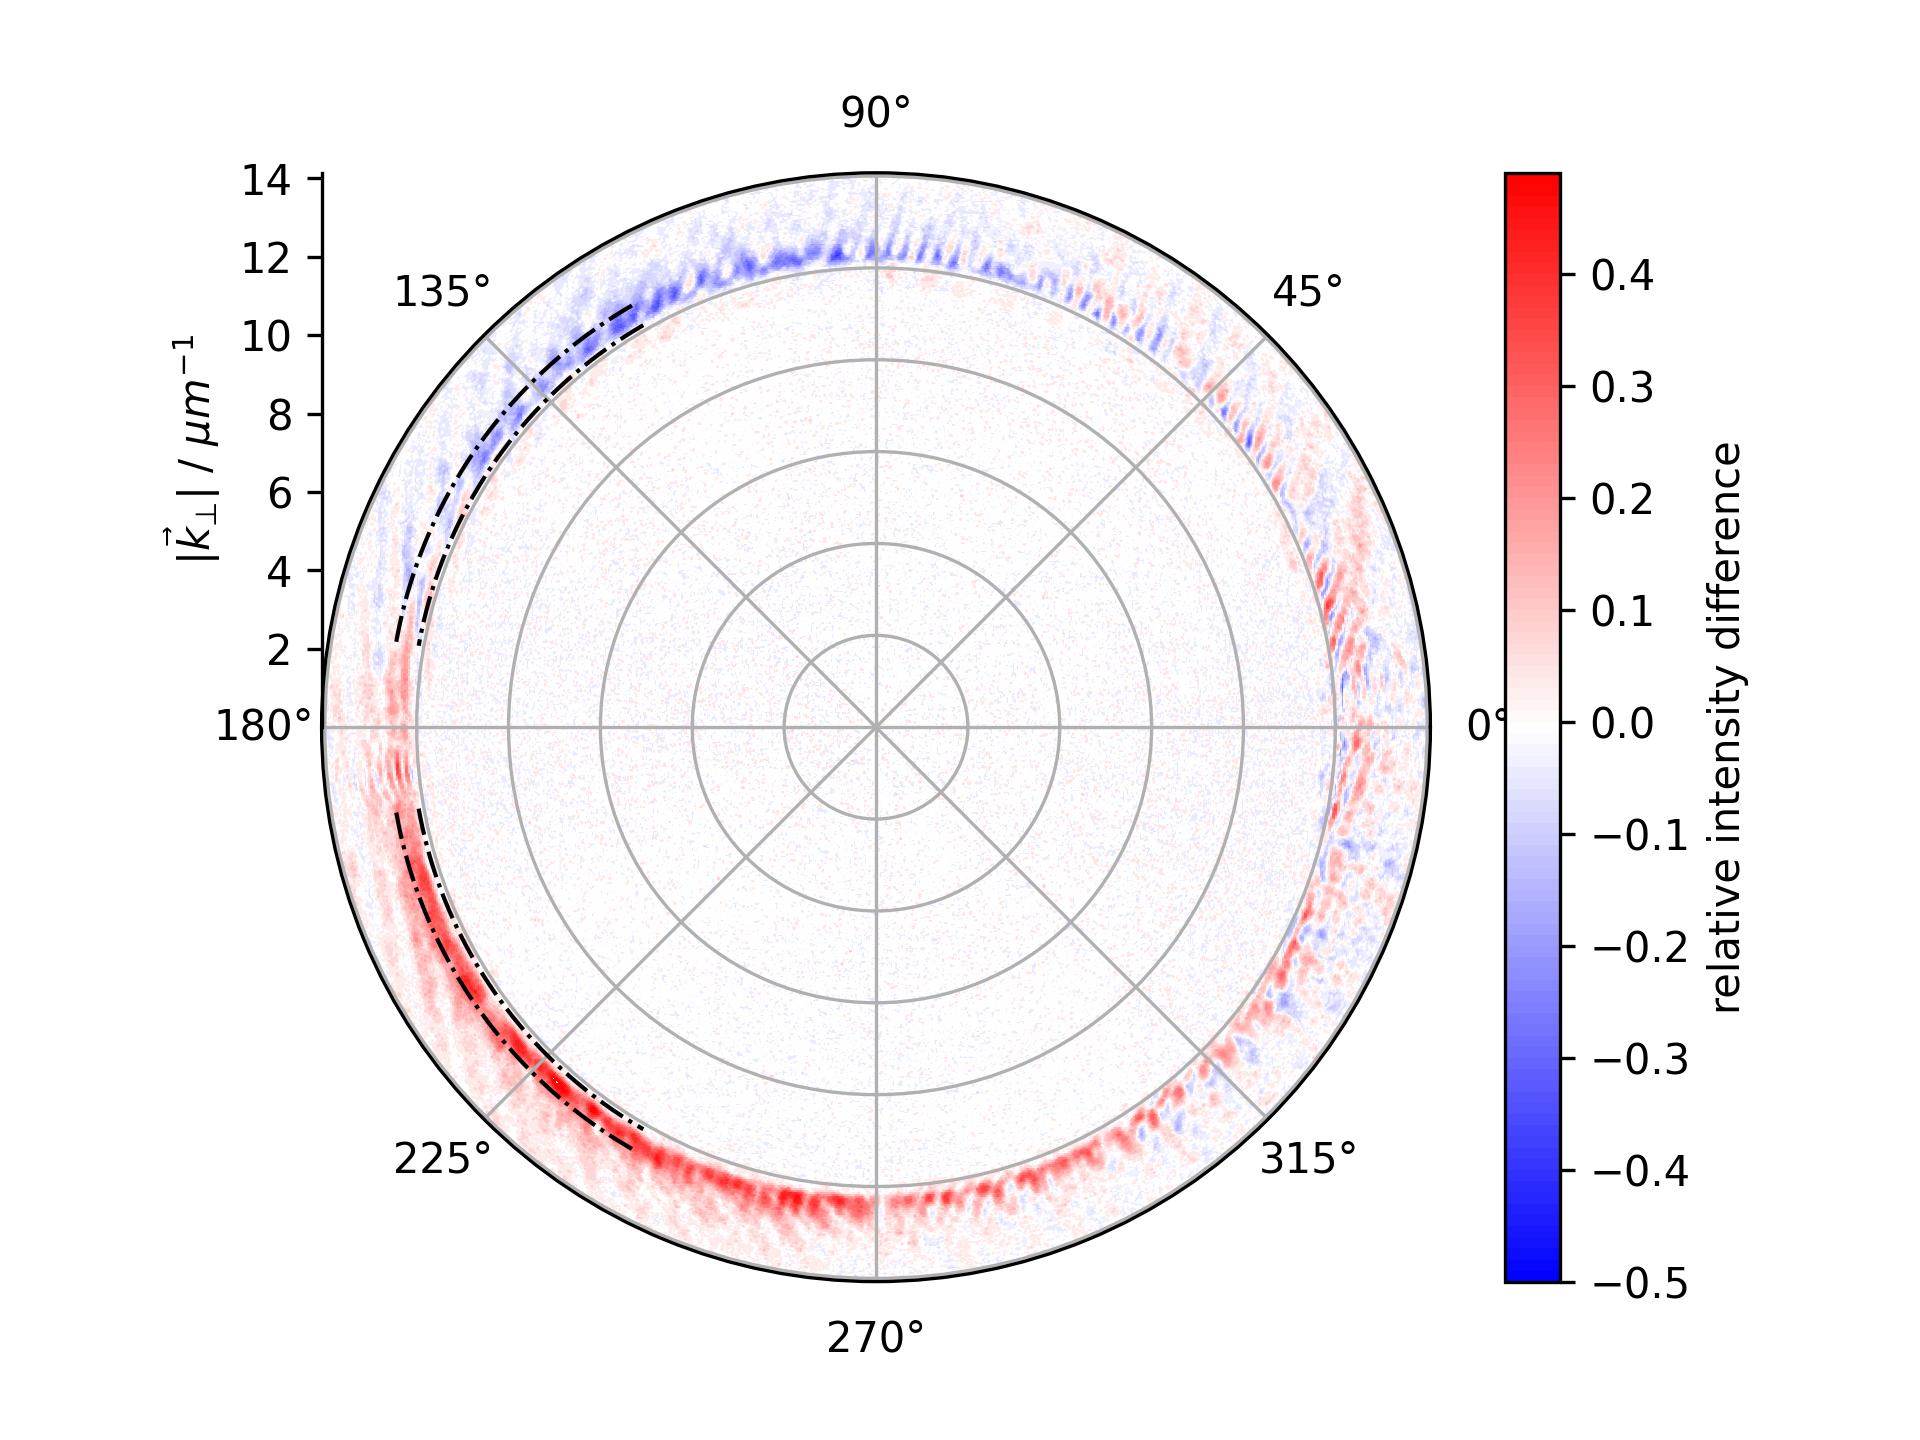
\includegraphics[width=\textwidth]{figures/spin_hall/diff_back.png}
			\caption{Differenz, Integrationsmaske $120^\circ-170^\circ$}
			\label{fig:diff_back}
		\end{subfigure}
		\hfill
		\begin{subfigure}[b]{0.49\textwidth}
			\centering
			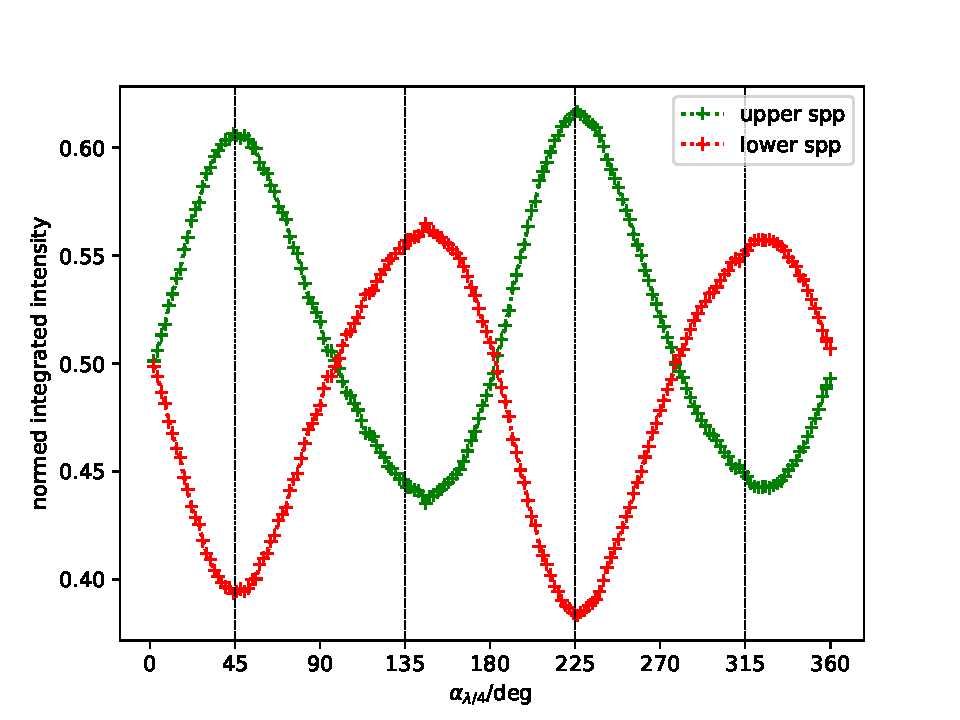
\includegraphics[width=\textwidth]{figures/spin_hall/intensity_back.pdf}
			\caption{Kontrast zwischen oberem und unterem SPP}
			\label{fig:intensity_back}
		\end{subfigure}
	
		\begin{subfigure}[b]{0.5\textwidth}
			\centering
			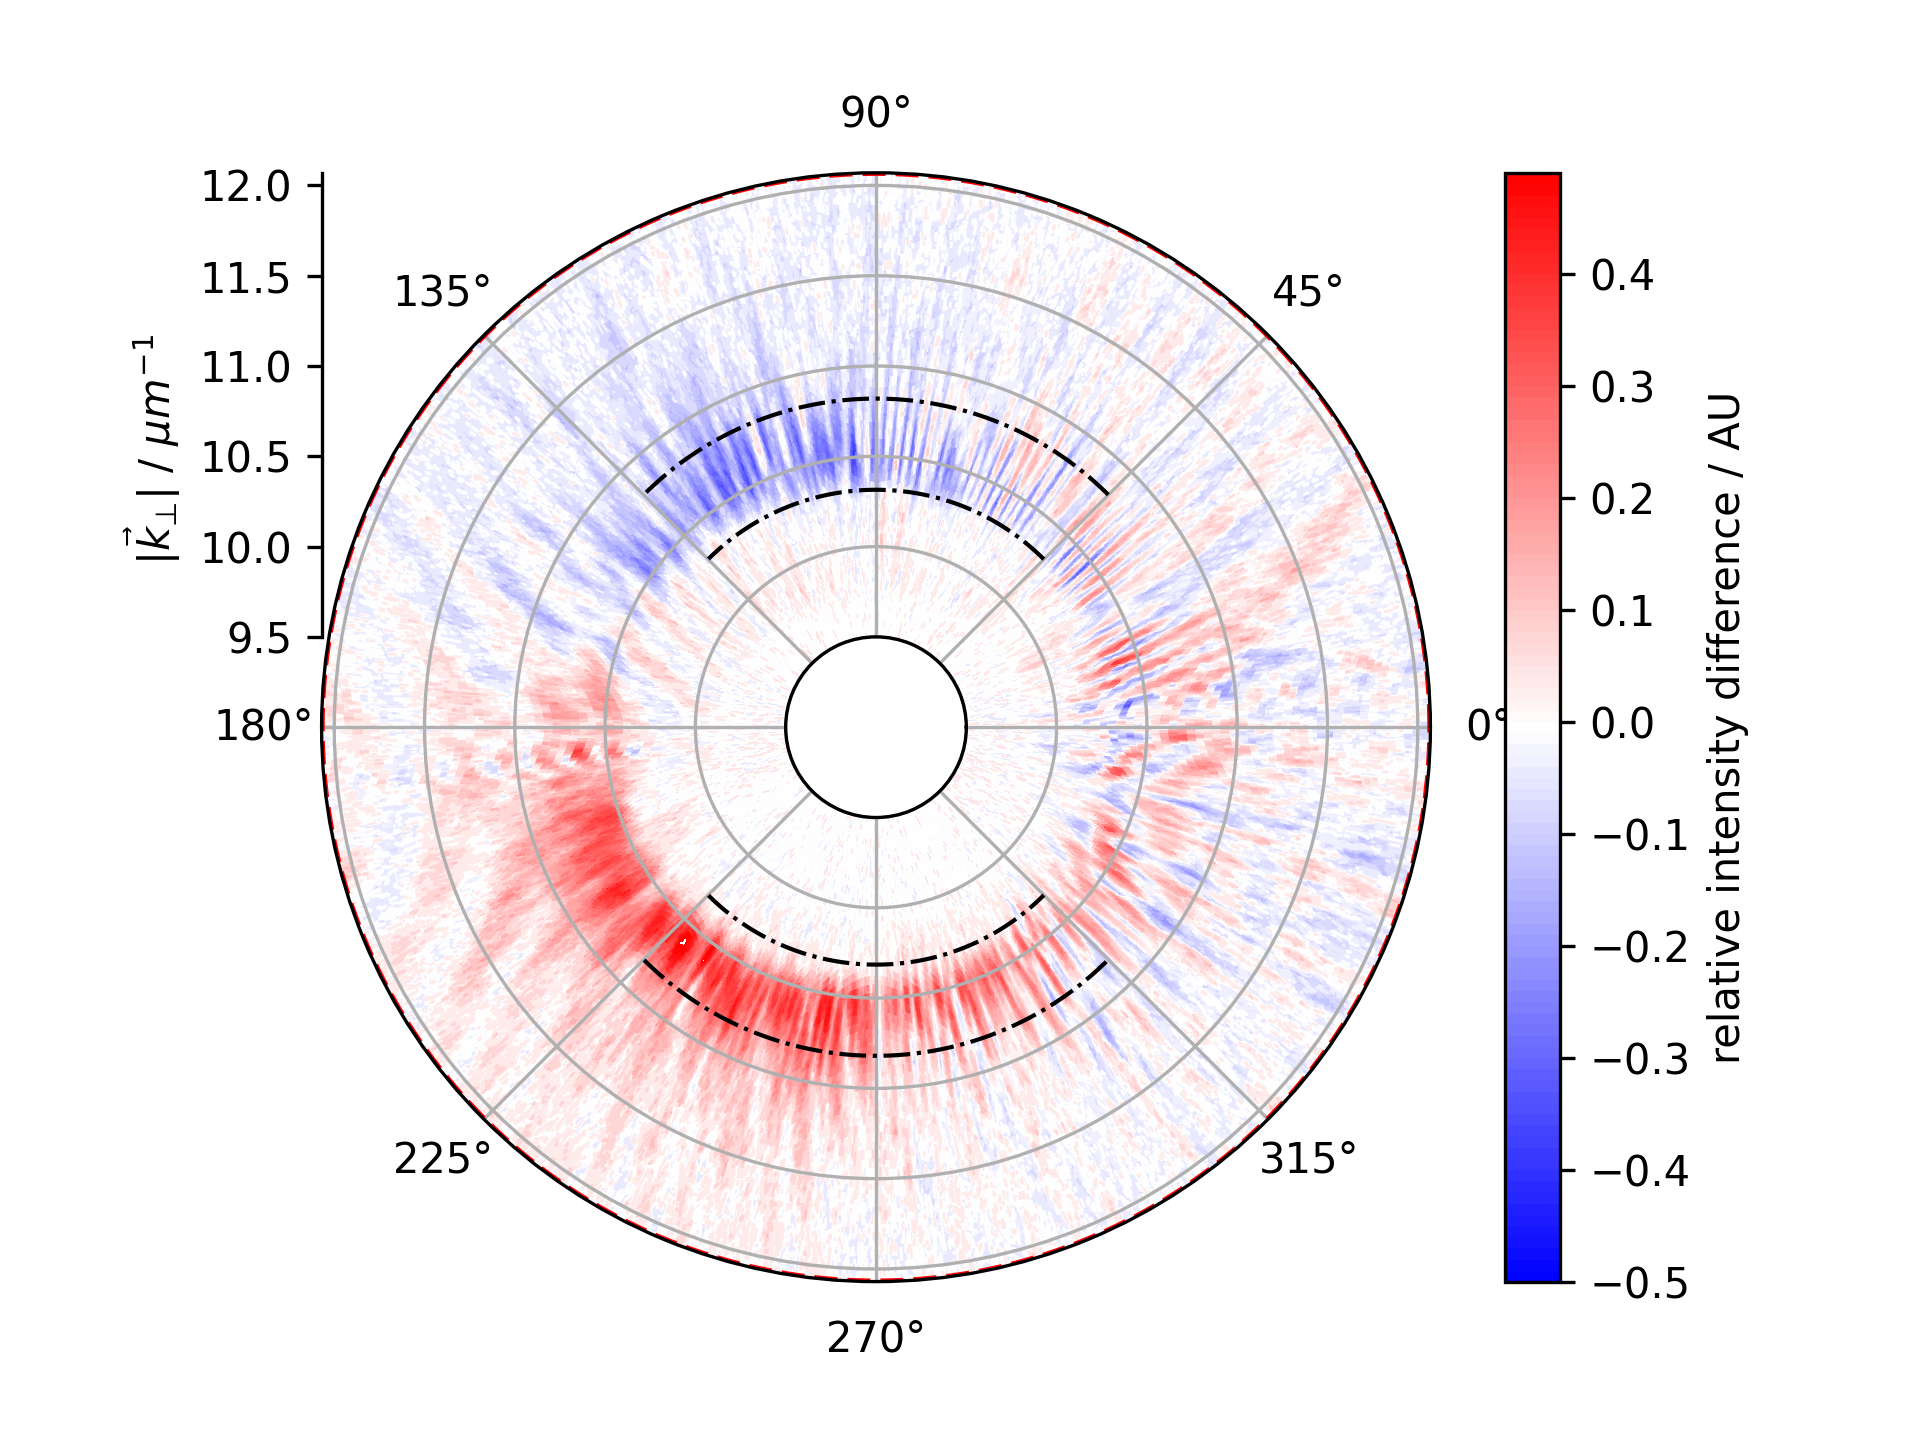
\includegraphics[width=\textwidth]{figures/spin_hall/diff_mid.png}
			\caption{Differenz BFP, Integrationsmaske $45^\circ-135^\circ$}
			\label{fig:diff_mid}
		\end{subfigure}
		\hfill
		\begin{subfigure}[b]{0.49\textwidth}
			\centering
			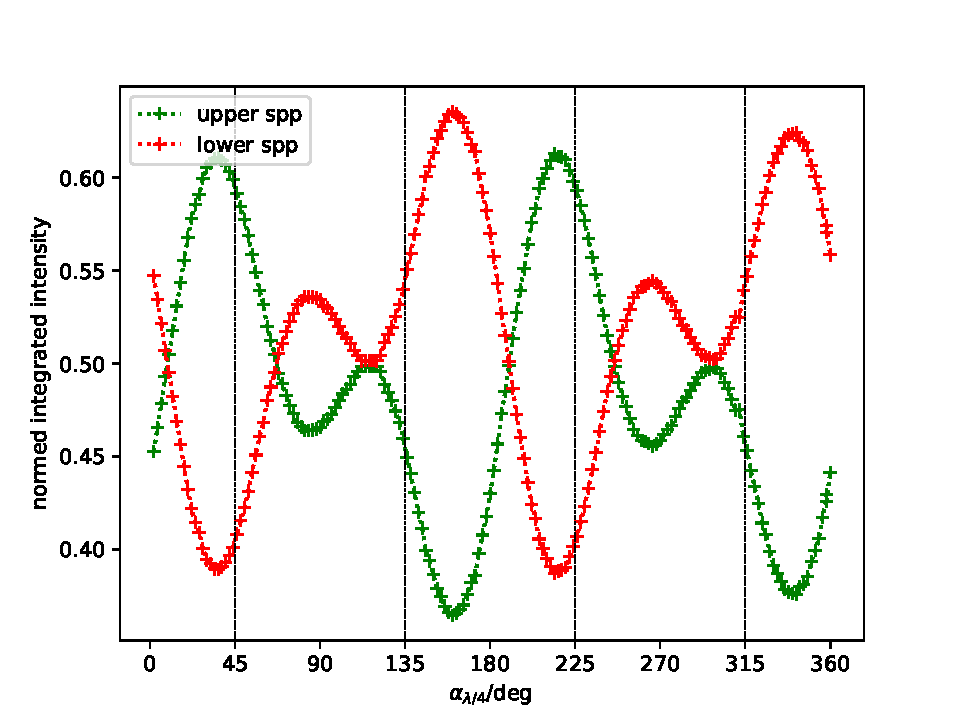
\includegraphics[width=\textwidth]{figures/spin_hall/intensity_mid.pdf}
			\caption{Kontrast zwischen oberem und unterem SPP}
			\label{fig:intensity_mid}
		\end{subfigure}
	
		\begin{subfigure}[b]{0.5\textwidth}
			\centering
			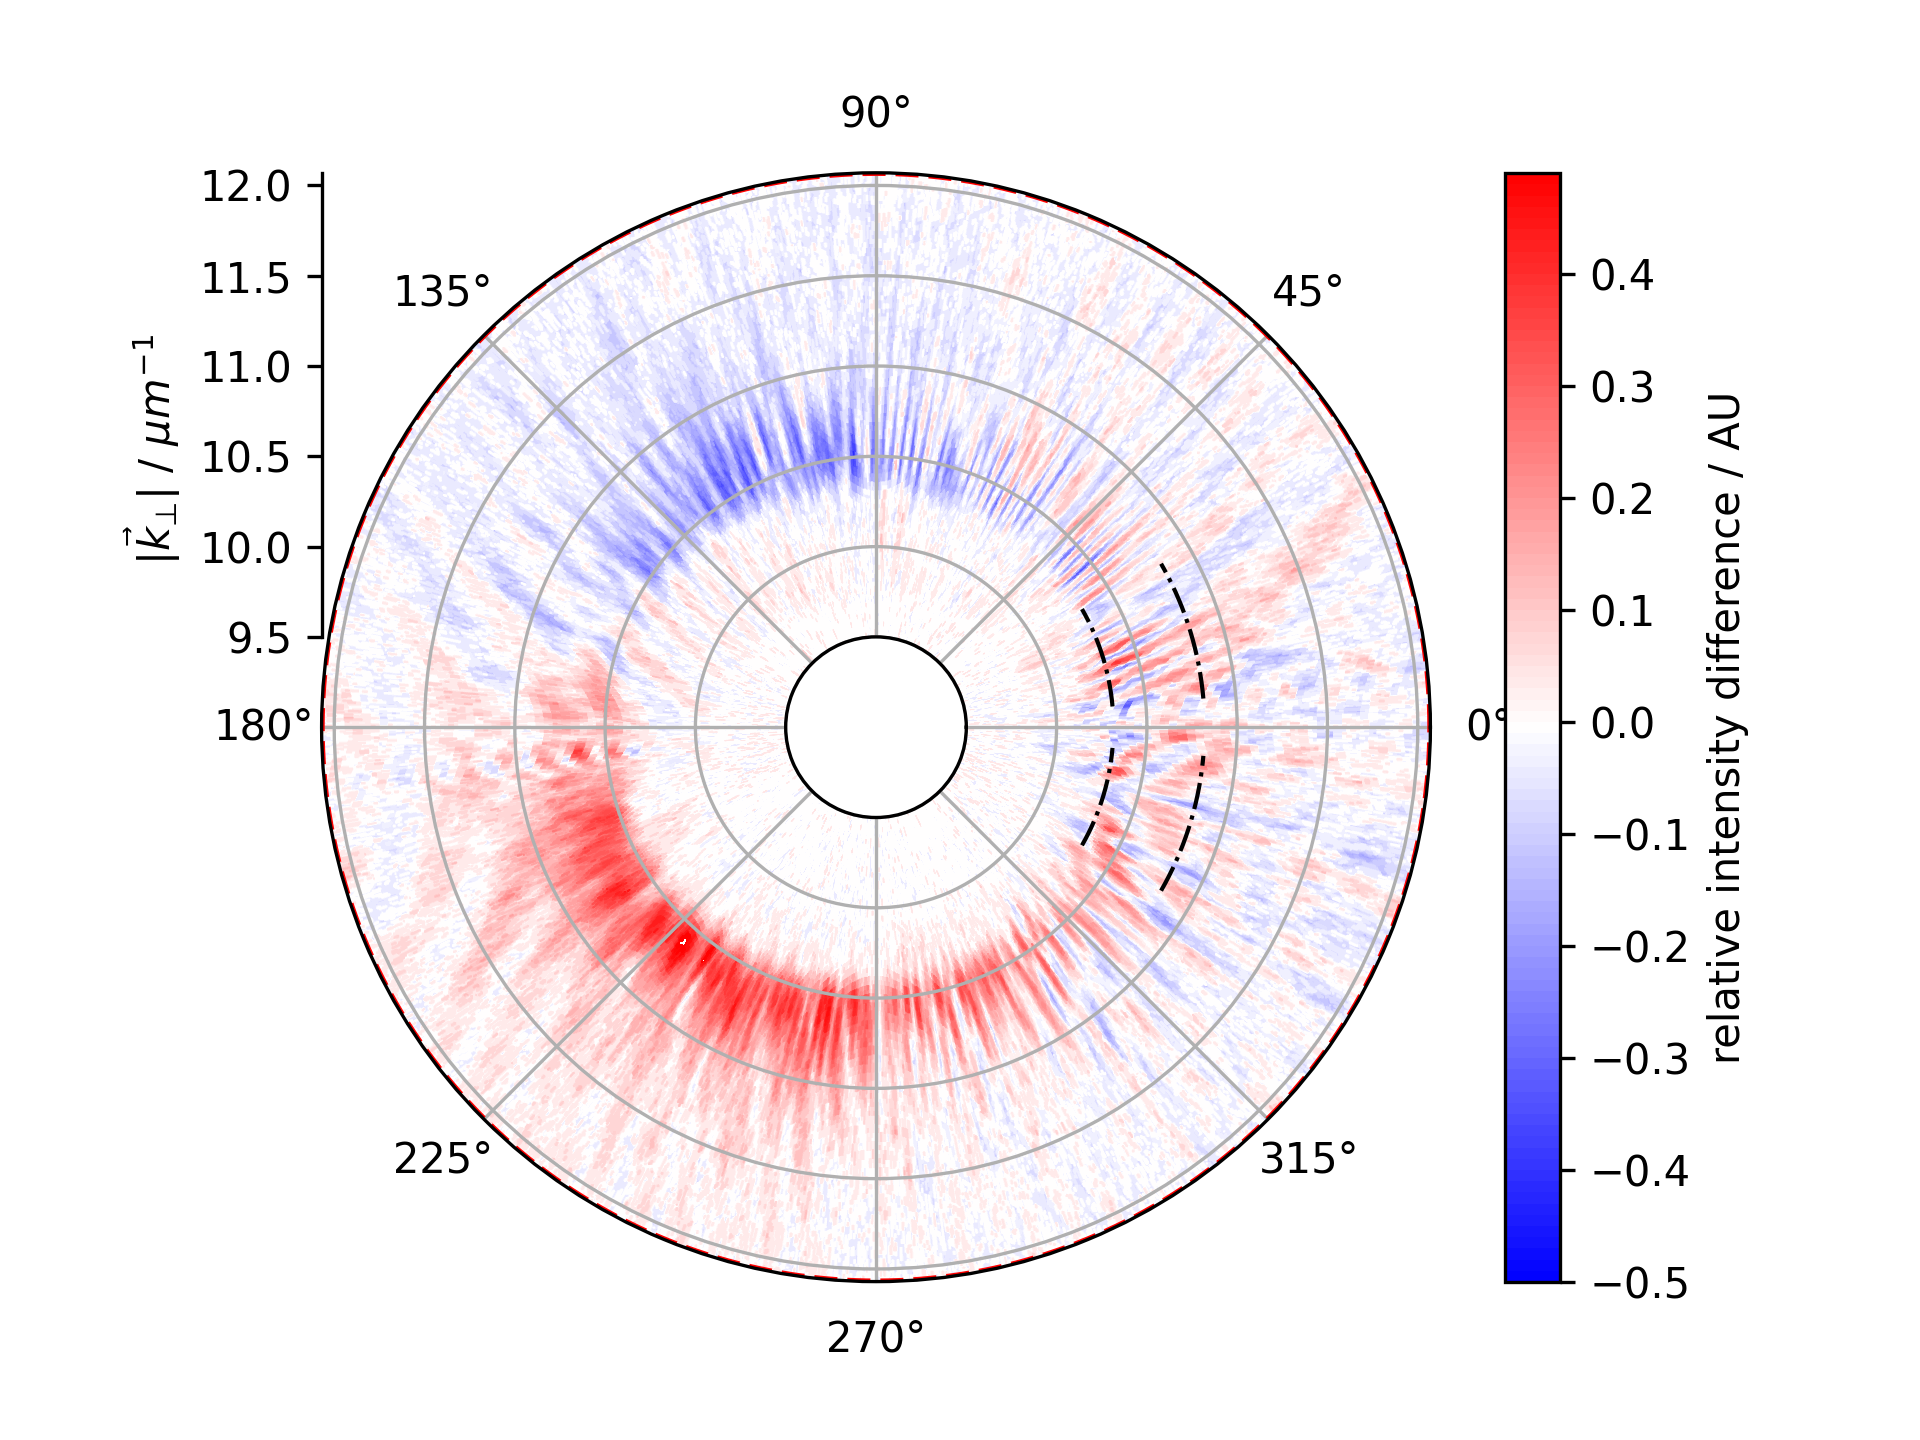
\includegraphics[width=\textwidth]{figures/spin_hall/diff_forw.png}
			\caption{Differenz BFP, Integrationsmaske $5^\circ-30^\circ$}
			\label{fig:diff_front}
		\end{subfigure}
		\hfill
		\begin{subfigure}[b]{0.49\textwidth}
			\centering
			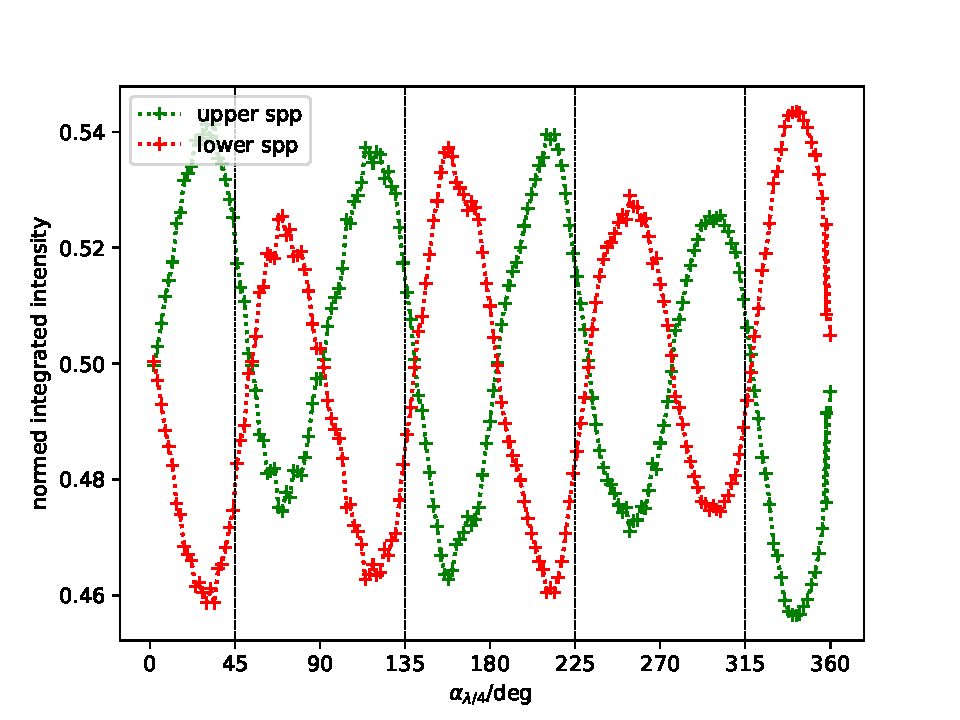
\includegraphics[width=\textwidth]{figures/spin_hall/intensity_forw.pdf}
			\caption{Kontrast zwischen oberem und unterem SPP}
			\label{fig:intensity_front}
		\end{subfigure}
		\caption{Die Differenz BFP-Abbildungen zeigen jeweils die relative Differenz in der Intensitäten in der BFP zwischen $\alpha_{\lambda/4} = 45^\circ$ und  $\alpha_{\lambda/4} = 135^\circ$ also die Fälle von links bzw. rechts zirkular Polarisierter Anregung. Außerdem sind in der BFP in schwarz jeweils die Integrationsmasken dargestellt. Der Rand der Abbildung entspricht$k_0\mathrm{NA}$. Die Abbildungen auf der linken Seite zeigen die Abhängigkeit des Kontrastes zwischen der Intensität in der oberen und der unteren Integrationsmaske in Abhängigkeit der Orientierung des $\lambda/4$-Plättchens. Die vertikalen Linien in dem Diagramm an den Positionen $\alpha_{\lambda/4} \in \{45^\circ, 135^\circ, 225^\circ, 315^\circ\}$ entsprechen einer Anregung mit zirkular polarisiertem Licht (alternierend links bzw. rechts zirkular).}	
	\end{figure}
	\subsection{Diskussion}
	In den Messdaten ist sind für unterschiedliche Ausbreitungsrichtungen relativ zum Einfallsebene des Lasers qualitativ unterschiedliche Verhaltensweisen zu beobachten.
	\paragraph{Rückwärtsrichtung}
	In Rückwärtsrichtung zum Strahl(Abbildungen \ref{fig:diff_back} u. \ref{fig:intensity_back}) konnte der erwartete Effekt beobachtet werden. Bei zirkularer Polarisation ($\alpha_{\lambda/4} \in \{45^\circ, 135^\circ, 225^\circ, 315^\circ\}$) ist jeweils die maximale Asymmetrie in Bezug auf die Einfallsebene zu erkennen. Diese Asymmetrie wechselt beim Wechsel des Drehsinns der zirkularen Polarisation wie erwartet ihre Orientierung. Das maximal beobachtet Kontrastverhältnis ist hierbei $\eta = 0.62:0.38$. Bei linearer Polarisation ($\alpha_{\lambda/4} \in \{0^\circ, 90^\circ, 180^\circ, 270^\circ\}$) verschwindet die Asymmetrie bis auf einen kleinen Rest, der vermutlich durch eine intrinsische Asymmetrie der Anregungsstruktur verursacht wird. Durch diese intrinsische Asymmetrie lässt sich auch erklären, dass das Kontrastverhältnis bei $135^\circ$ und $ 315^\circ$ jeweils etwas geringer ist, als bei $45^\circ$ und $225^\circ$.
	Die intrinsische Asymmetrie der Struktur addiert sich auf die Asymmetrie, die durch den Spin-Hall-Effekt verursacht wird und verstärkt bzw. schwächt diese abwechselnd ab.
	\paragraph{Vorwärtsrichtung}
	In Vorwärtsrichtung (Abbildungen \ref{fig:diff_front} u. \ref{fig:intensity_front}) konnte nicht der erwartete Effekt beobachtet werden. Hier tritt die maximale Asymmetrie jeweils bei elliptischer Polarisation auf und verschwindet bei zirkularer Polarisation. Bei linearer Polarisation verschwindet die Asymmetrie ebenfalls. Insgesamt zeigt der Verlauf die doppelte Frequenz der erwarteten Asymmetrie Modulation. Daher ist das Signal auch Symmetrisch bezüglich des Drehsinns der Polarisation. Für diese Phänomen wurde im Rahmen dieser Arbeit keine endgültige Erklärung gefunden.
	
	 Eine möglicher Erklärungsansatz ist die unbekannte Detailstruktur des Defektes. In den Theoretischen Überlegungen ist von einem idealen Dipol ausgegangen worden. Wenn die Multipolentwicklunng des polarisiertem Defektes noch höhere von null verschiedene Terme aufweist, könnten weitere unbekannte Effekte auftreten. Das durch kompliziertere Strukturen weitere nicht triviale Effekte auftreten können, kann man auch in den Messungen (Abbildung \ref{fig:RF_measure_int}) von \cite{RodriguezFortuno.2013} erkennen. Dort wurde der PSHE unter anderem an einer Gitterstruktur beobachtet. Die Messung an der Gitterstruktur zeigt auch eine gewisse Überlagerung von Signalen unterschiedlicher Frequenz. So ist dort bei ca. $10^\circ$ ein weiteres Maximum der \textit{left SPP intensity} zu erkennen, dass durch die einfachen Modelle des Spin Hall Effektes nicht zu erklären ist. Diese Messungen bestätigen die Vermutung, dass kompliziertere Strukturen sich in nicht trivialer Weise auf das Intensitätsbild auswirken.
	 
	 Ein weiterer Erklärungsansatz ist, dass in den Simulation von einem ideal streifenden Einfall ausgegangen worden ist. In dem realen Experiment konnte durch Geometrische Begrenzungen nur ein Einfallswinkel von $60^\circ$ zur Oberflächennormale realisiert werden. Auch diese andere Orientierung des Dipol könnte einen Effekt auf die Intensitätsverteilung in Abhängigkeit der Polarisation haben.
	 
	 Bei genauerer Betrachtung des Differenzbildes zwischen links und rechts zirkularer Polarisation (Abbildung \ref{fig:diff_front}) fällt außerdem auf, dass das Differenzbild in Vorwärtsrichtung ein feine Struktur aufweist. Diese Struktur könnte durch Interferenzeffekte erklärt werden.
	\paragraph{Senkrecht zur Einfallsebene}
	Senkrecht zur Einfallsebene (Abbildungen  \ref{fig:diff_mid} u. \ref{fig:intensity_mid}) wurde eine Überlagerungen aus den oben beschriebenen Periodizitäten beobachtet. Diese Überlagerung führt dazu, dass das Signal des PSHE nicht mehr eindeutig zu identifizieren ist.
	\begin{figure}
	\label{fig:RF_measure}
	\centering
	\begin{subfigure}[b]{0.5\textwidth}
		\centering
		\includegraphics[width=\textwidth]{figures/RF_SM_Slits.pdf}
		\caption{Struktur}
		\label{fig:RF_measure_slits}
	\end{subfigure}
	\hfill
	\begin{subfigure}[b]{0.49\textwidth}
		\centering
		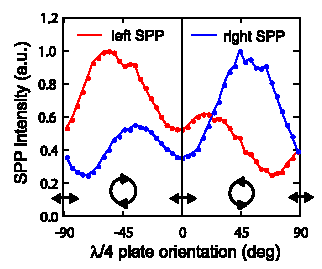
\includegraphics[width=\textwidth]{figures/RF_SM_Intensity.pdf}
		\caption{Intensitätsverteilung}
		\label{fig:RF_measure_int}
	\end{subfigure}
	\caption{Die Abbildung zeigt die Messungen von \cite{RodriguezFortuno.2013}, die an einer Gitterstruktur durchgeführt worden sind.}			
	\end{figure}
	
	\paragraph{Vergleich mit Spin-Hall-Effekt}
	...
\section{Zusammenfassung und Ausblick}

\newpage
\appendix
\bibliography{bib}
\section{Programmierung}
\section{Polarimeter}
\newpage
\section{Technische Zeichnungen}
\begin{sidewaysfigure}[h!]
	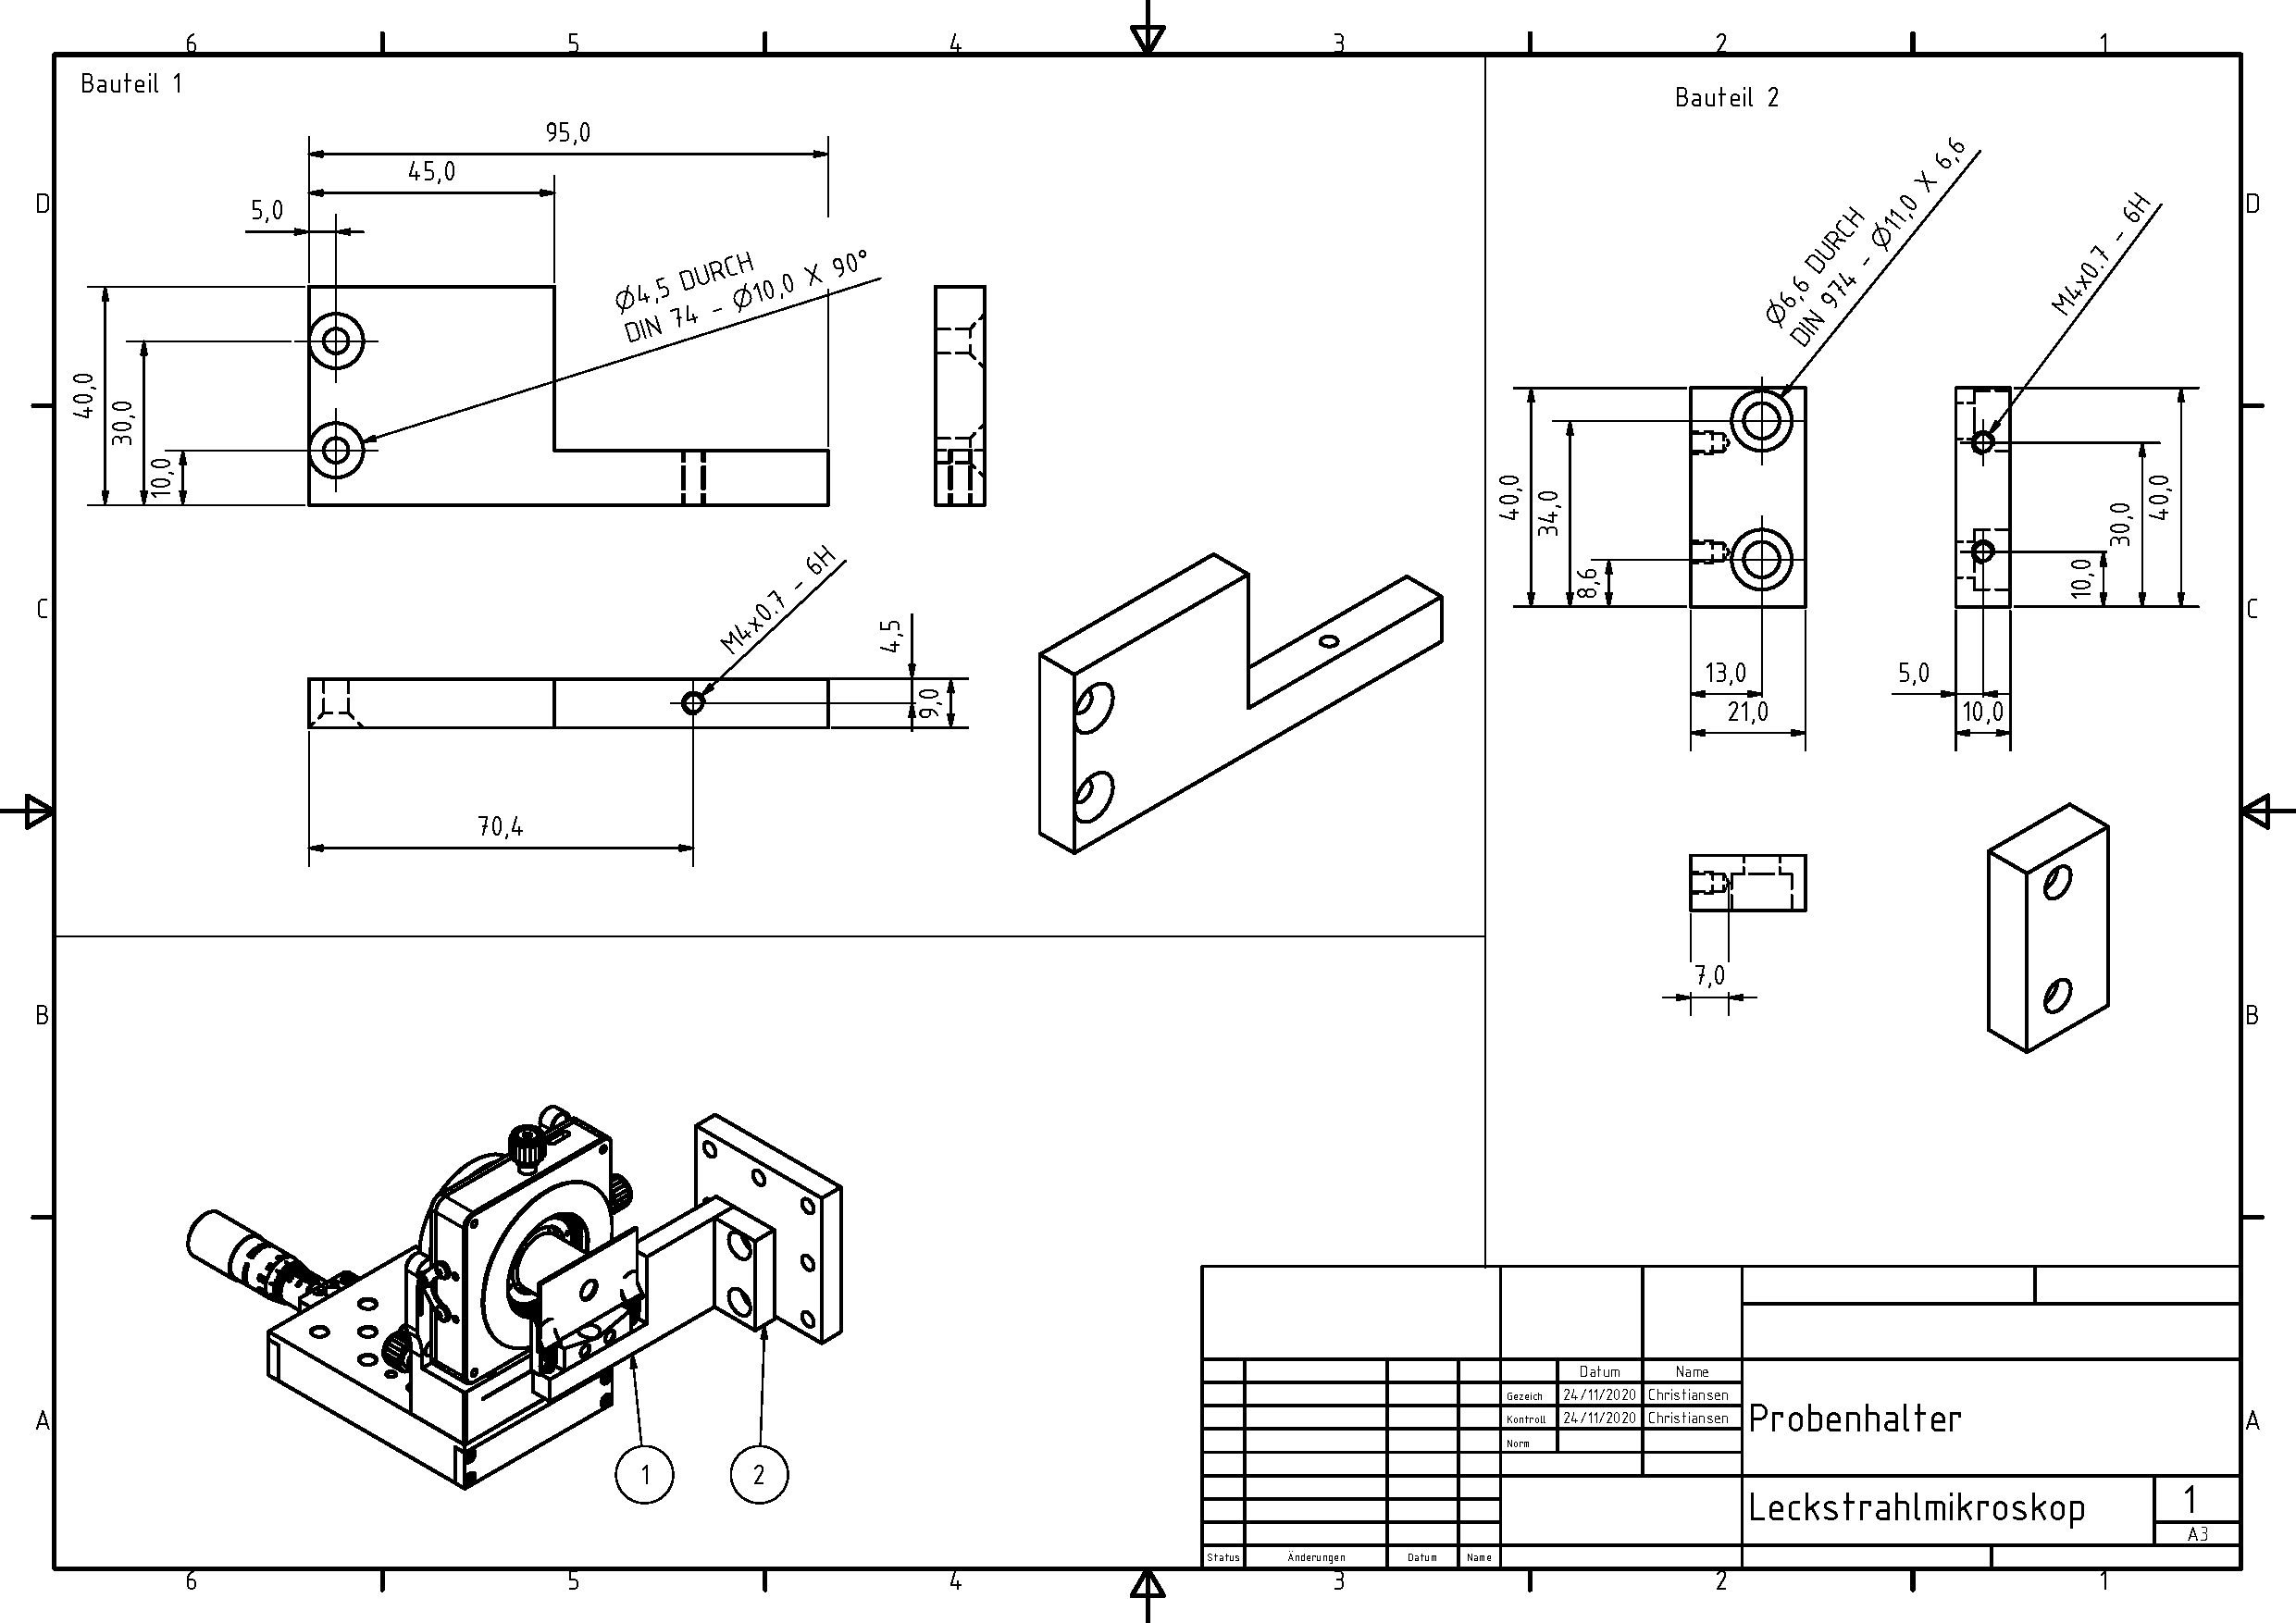
\includegraphics[width=\textwidth]{figures/Technische_Zeichnung_Probenhalter.pdf}
	\caption{Technische Zeichnung Probenhalter}
	\label{fig:tz_probenhalter}
\end{sidewaysfigure}
\begin{sidewaysfigure}[h!]
	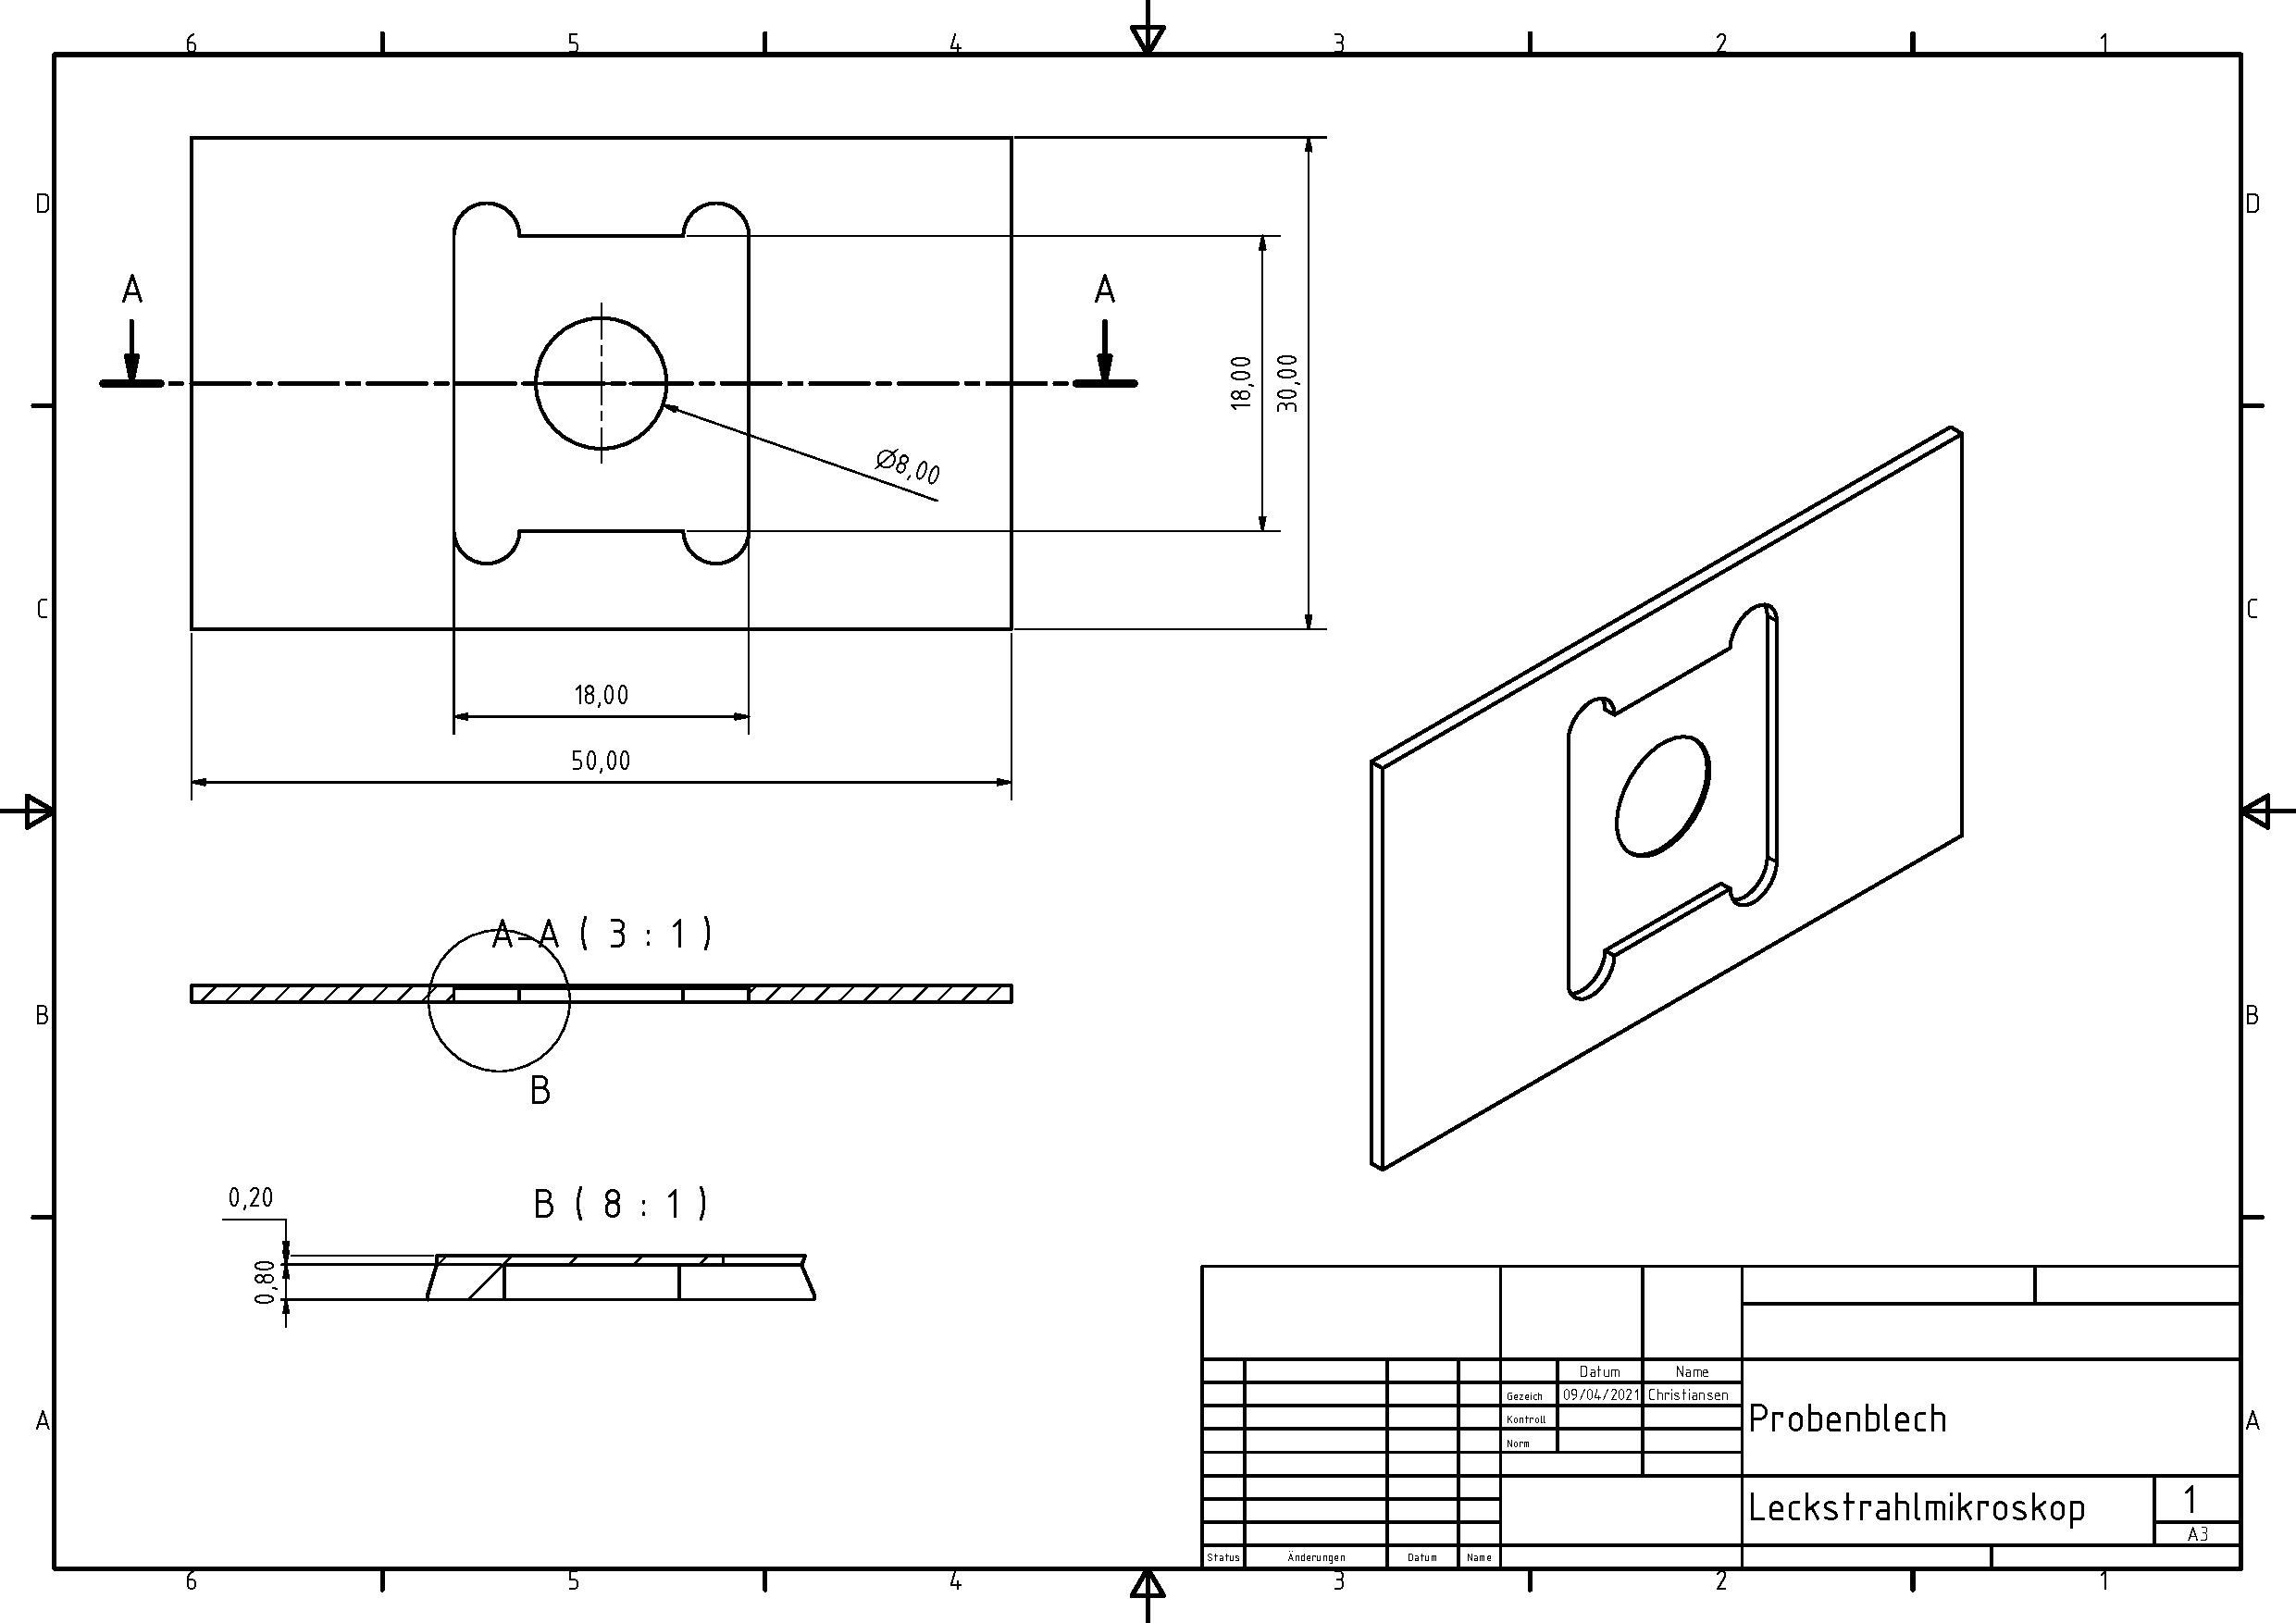
\includegraphics[width=\textwidth]{figures/Probenblech.pdf}
	\caption{Technische Zeichnung Probenblech}
	\label{fig:tz_probenblech}
\end{sidewaysfigure}
\begin{sidewaysfigure}[h!]
	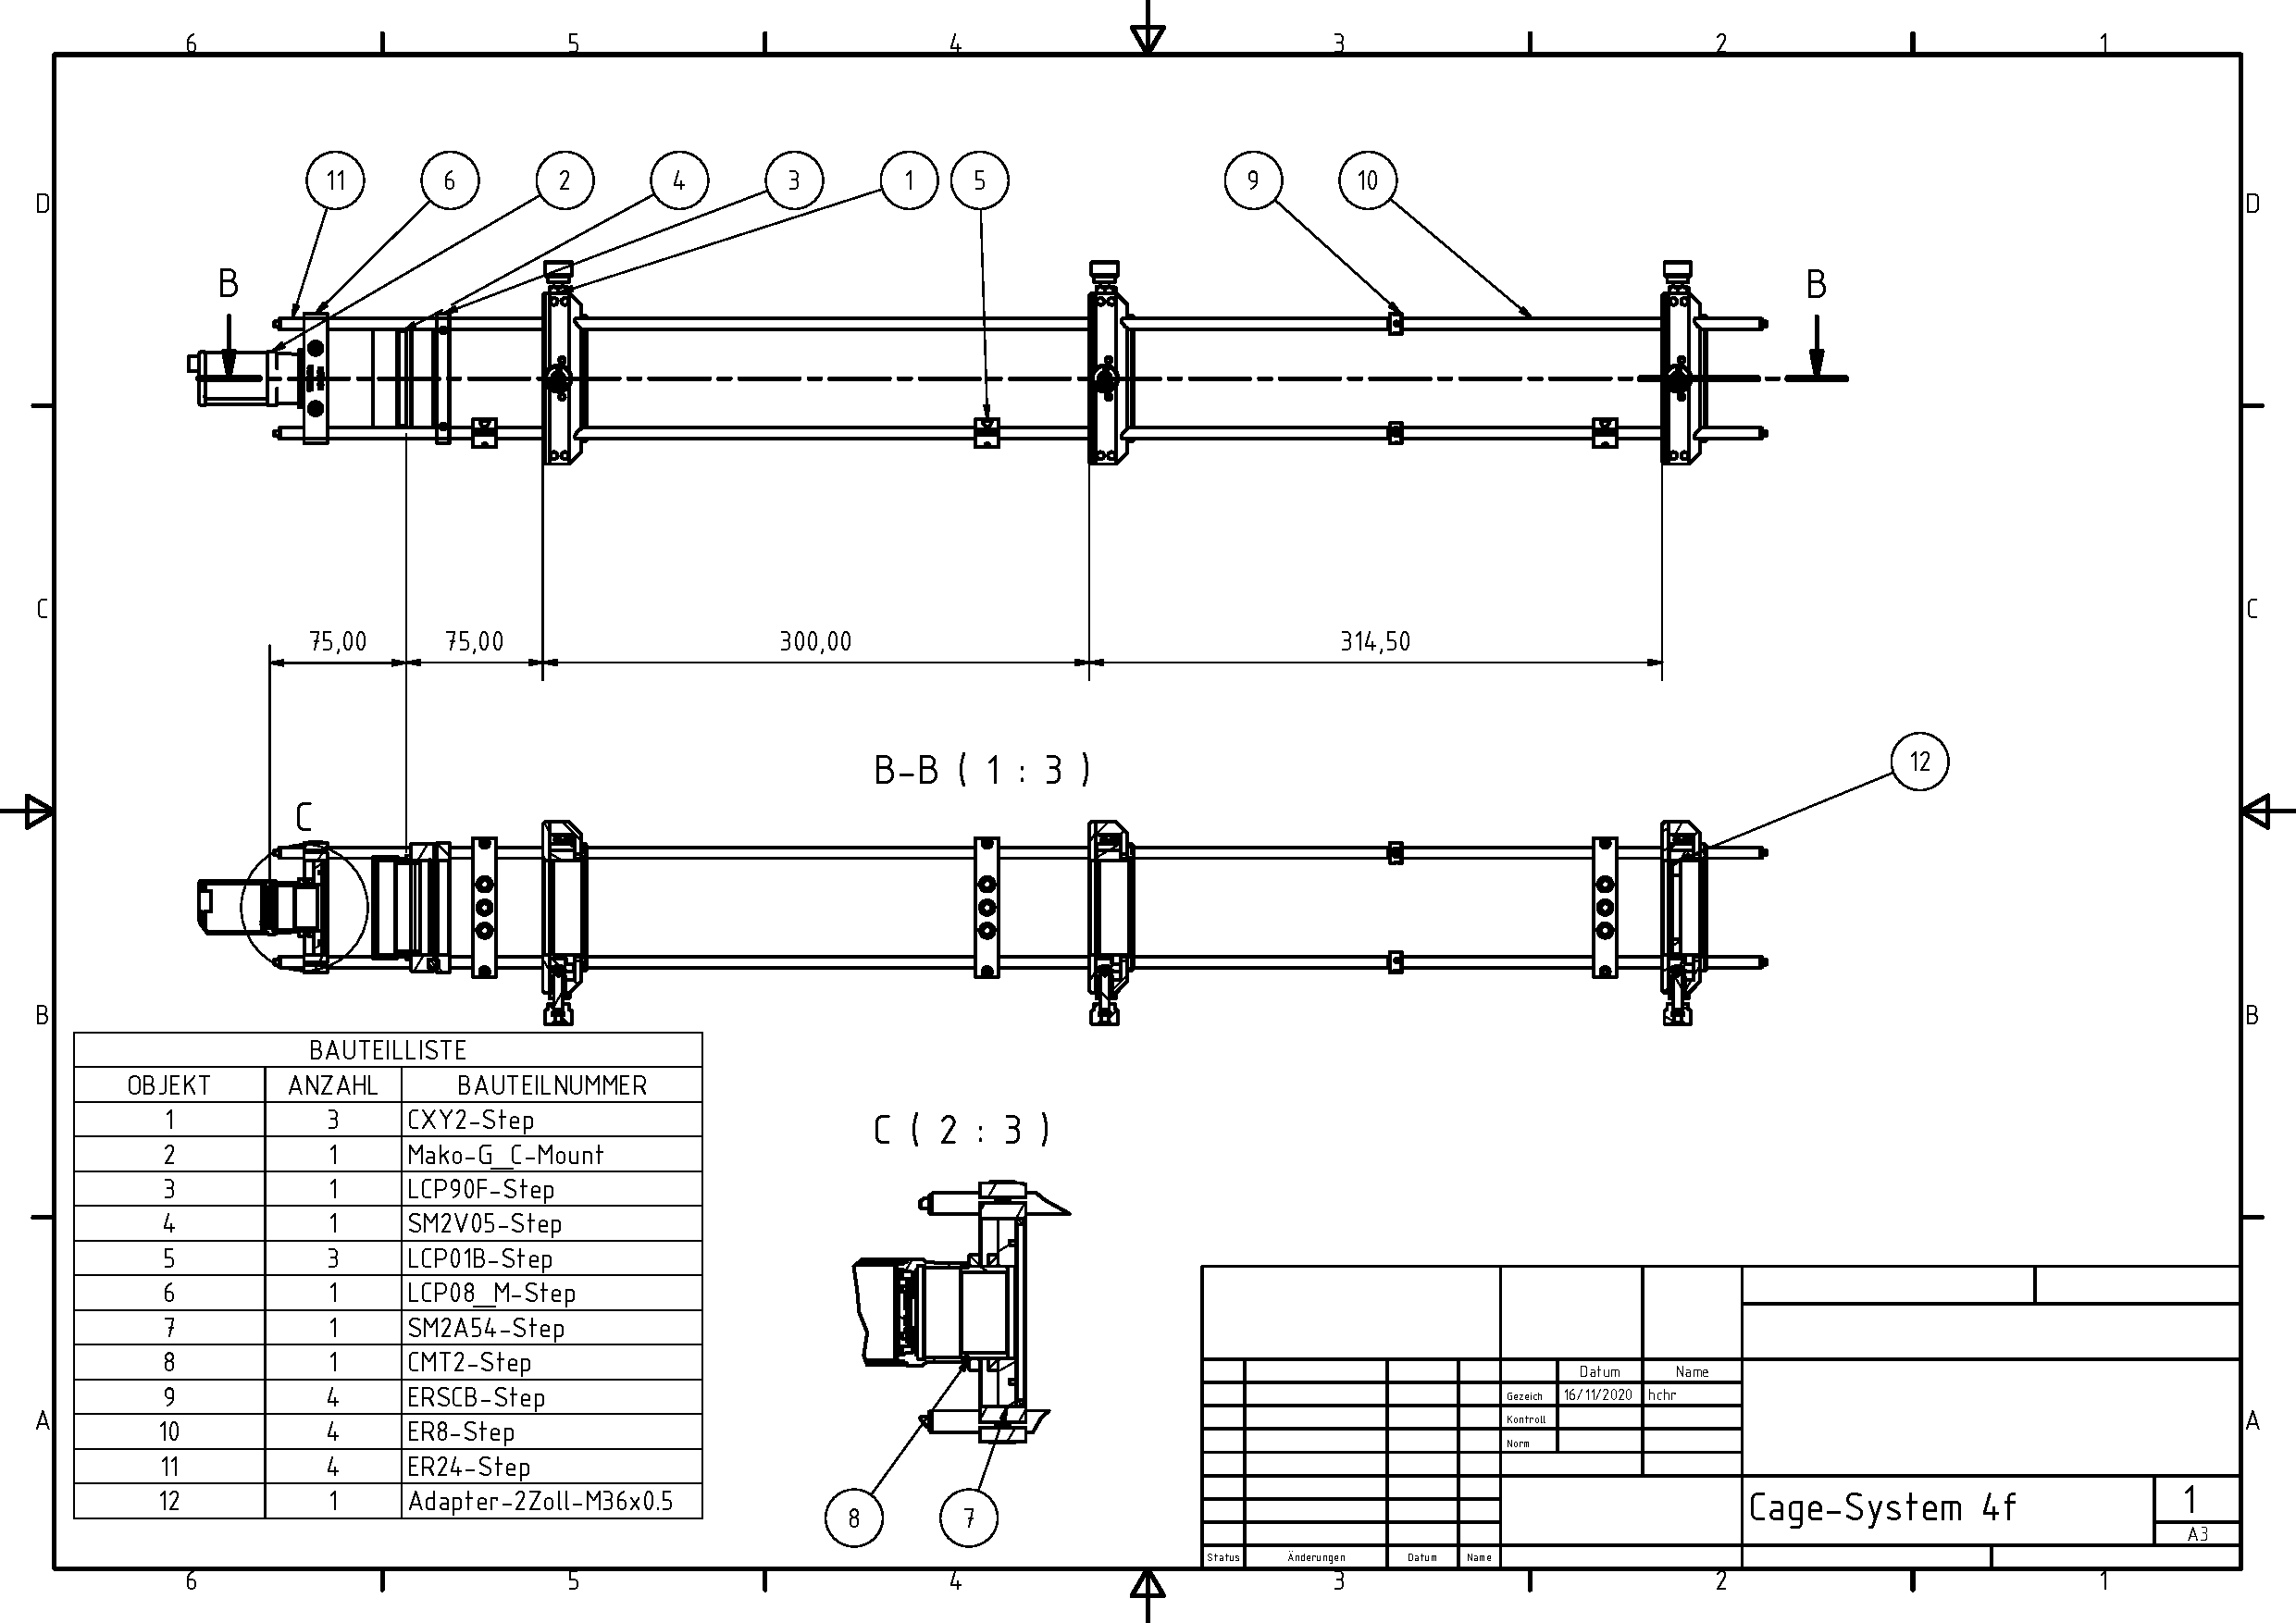
\includegraphics[width=\textwidth]{figures/4f_system.pdf}
	\caption{Technische Zeichnung Cage-System}
	\label{fig:tz_cage_system}
\end{sidewaysfigure}
\newpage
\section{Liste der verwendeten Komponenten}
\begin{table}[h!]
	\centering	
	\label{tab:components}
	\begin{tabular}{|c|c|c|}
		\hline
		\textbf{Bauteil}         & \textbf{Typ}                   & \textbf{Hersteller}                    \\
		\hline
		\hline
		Helium-Neon-Laser        & HNL210L-EC                     & \textit{Thorlabs}                      \\
		ND Filter                & NDL-25C-2                      & \textit{Thorlabs}                      \\
		$\lambda/4$-Plättchen    & WPMQ05M-633                    & \textit{Thorlabs}                      \\
	    Polarisationsfilter      & -        					  & \textit{Newport}                       \\
		Hintergrund LED          & -          					  & -                  					   \\
		Blenden                  & -          					  & -                  					   \\
		Spiegel                  & -          					  & -                  					   \\
		Kollimatorlinse          & Lens Asphere Ach 25x40Vis 0 TS & \textit{Edmund Optics}                 \\
		Immersionsobjektiv       & 100-fach/1.25 N-Achroplan      & \textit{Carl Zeiss}                    \\
		Immersionsöl             & 518N, n=1.518                  & \textit{Carl Zeiss}                    \\
		Tubuslinse               & 452149-0000-000                & \textit{Carl Zeiss}                    \\
		2x Linsen                & LA1417-A-ML, f = 150 mm        & \textit{Thorlabs}                      \\
		1x Linsen                & LA1417-A-ML, f = 75 mm         & \textit{Thorlabs}                      \\
		2x Lineartisch           & 2000551						  &\textit{Thorlabs} 					   \\
		Kristallhalter           & LP-1A (XYZ) Series             & \textit{Newport}                       \\
		Objektiv-Adapter         & LPMH-1                         & \textit{Newport}                       \\
		3-Achsen-Bühne           & TSD                            & \textit{OptoSigma}                     \\
		2-Achsen-Bühne           & TSD                            & \textit{OptoSigma}                     \\
		Filter-Halter            & FH2                            & \textit{Thorlabs}                      \\
		Einkoppellinse           & LA-1805                        & \textit{Thorlabs}                      \\
		Linsenhalter             & M-LH-1A                        & \textit{Newport}                       \\
		Cage Plate               & LCP08/M                        & \textit{Thorlabs}                      \\
		Linsen Tubus Verbinder   & CMT2                           & \textit{Thorlabs}                      \\
		SM2, CMount Adapter      & SM2A54                         & \textit{Thorlabs}                      \\
		Justierbarer Linsentubus & SM2V05                         & \textit{Thorlabs}                      \\
		Magnet Cage-Plate        & LCP90F                         & \textit{Thorlabs}                      \\
		3x xy-Linsenhalter       & CXY2                           & \textit{Thorlabs}                      \\
		3x Cage-System-Halter    & LCP01B                         & \textit{Thorlabs}                      \\
		4x Cage-System-Stange    & ER8                            & \textit{Thorlabs}                      \\
		4x Cage-System-Stange    & ER24                           & \textit{Thorlabs}                      \\
		4x Stangenverbinder      & ERSCB                          & \textit{Thorlabs}                      \\
		CageSystem Justier Hilfe & LCPA1                          & \textit{Thorlabs}                      \\		
		Probenhalter		     & Eigendesign                    & Werkstatt                              \\
		Probenblech              & Eigendesign                    & Werkstatt                              \\
		BeamBlock                & Eigendesign                    & Werkstatt                              \\
		Tubuslinsenhalter        & Eigendesign                    & Werkstatt                              \\
		\hline          
	\end{tabular}
	\caption{Liste der verwendeten Komponenten}
\end{table}

	
\end{document}